%% =========================================================================
%% Dissertação de Mestrado — PPGCC, CIn-UFPE
%% Template: risethesis (classe do CIn; mesma base das dissertações do
%% programa — ver blueprint em docs/blueprint-dissertacao.md)
%% Compilar: pdflatex -> bibtex -> pdflatex x2
%% =========================================================================
\documentclass[pt,oneside,onehalfspacing,msc]{risethesis}

\usepackage[brazilian]{babel}
\usepackage{color}
\usepackage[table]{xcolor}
\usepackage{microtype}
\usepackage{multirow}
\usepackage{rotating}
\usepackage{booktabs}
\usepackage{caption}
\usepackage{float}
\usepackage{subcaption}
\usepackage{amsmath,amssymb}
\usepackage{textcomp}
% tikz removido do preâmbulo: os 6 diagramas são pré-compilados em
% images/tikz-*.pdf (fontes editáveis em tikz-src/) — corta o tempo de
% compilação p/ caber no limite do plano grátis do Overleaf.
% paragraphs sem numeração (a classe numera até nível 5 por default)
\setcounter{secnumdepth}{3}
\setcounter{tocdepth}{2}

%% ---- Formato de títulos no padrão das dissertações do CIn (análise
%% forense de 06/10/2026: corpus abnTeX2 local usa 12pt, hierarquia por
%% destaque tipográfico, nunca por tamanho — NBR 14724/manual SIB) ----
\titleformat{\chapter}[hang]
  {\normalsize\bfseries}{\thechapter}{1em}{\MakeUppercase}
\titleformat{name=\chapter,numberless}[hang]
  {\normalsize\bfseries\filcenter}{}{0pt}{\MakeUppercase}
\titlespacing*{\chapter}{0pt}{0pt}{24pt}
\titleformat{\section}
  {\normalsize}{\thesection}{1em}{\MakeUppercase}
\titleformat{\subsection}
  {\normalsize\bfseries}{\thesubsection}{1em}{}
\titleformat{\subsubsection}
  {\normalsize\itshape}{\thesubsubsection}{1em}{}
%% Legendas: 10pt (menores e uniformes, regra do manual)
\captionsetup{font=small,labelfont=small,skip=6pt}

\newcommand{\us}{\textmu s}

\address{RECIFE}
\universitypt{Universidade Federal de Pernambuco}
\universityen{Federal University of Pernambuco}
\institutept{Centro de Informática}
\instituteen{Center for Informatics}
\programpt{Pós-graduação em Ciência da Computação}
\programen{Graduate Program in Computer Science}
\majorfieldpt{Ciência da Computação}
\majorfielden{Computer Science}

\title{Modelos para Dados Tabulares na Era dos Foundation Models:
um Benchmark Multicritério, um Arcabouço de Decisão Validado e a
Destilação Distribucional}

\date{2026}
\author{João Gabriel de Araújo Vasconcelos}
\adviser{Germano Crispim Vasconcelos}

% DICA (plano grátis do Overleaf): se a compilação completa estourar o
% tempo, edite por capítulo descomentando a linha abaixo (compila só o
% capítulo listado, mantendo numeração/refs do .aux da última completa):
% \includeonly{chapters/cap7-destilacao}

\begin{document}

\frontpage
\presentationpage

\begin{fichacatalografica}
% Folha em branco: a ficha catalográfica é gerada pela biblioteca via
% SIGAA no depósito (manual SIB/UFPE, procedimento vigente desde 08/2024).
\end{fichacatalografica}

% Folha de aprovação: elaborada pela secretaria após a defesa, sem
% assinaturas no depósito (manual SIB/UFPE). Placeholder da banca:
% [3-4 doutores, >= 1 externo; orientador preside — regimento PPGCC art. 37]

\acknowledgements
[Agradecimentos --- a preencher pelo autor.]


\resumo
[Resumo em um parágrafo, 150--500 palavras, sem fórmulas (NBR 6028) ---
escrito por último, quando os capítulos fecharem.]

\vspace{1cm}
\noindent\textbf{Palavras-chaves:} dados tabulares; foundation models;
benchmark; destilação de conhecimento; regressão distribucional.


\abstract
% Abstract — faithful mirror of pretext/resumo.tex (NBR 6028: one
% paragraph, 150-500 words, no formulas).
For a decade, model choice for tabular data was guided by the maxim that
gradient boosting always wins; the arrival of tabular foundation models
--- pre-trained networks that predict with no task-specific training ---
made that guidance obsolete without replacing it with neutral evidence.
This dissertation attacks the problem on three chained fronts. First, a
multi-criteria benchmark evaluates 14 models from three families
(gradient boosting, deep learning, and foundation models) on 18 public
OpenML datasets (250 of the 252 possible cells; two declared structural
exclusions), under nested cross-validation with an untouched hold-out and
both frequentist and Bayesian statistical inference. In the study's 11-model core slate, the top of the accuracy ranking is a statistical tie --- 8 of
the 10 non-leading models are practically equivalent to the leader under
a region of practical equivalence of one percentage point of AUC --- and
the 2026 generation breaks it: TabFM, evaluated zero-shot, leads the
average rank in all three tasks (2.7 in binary classification, 1.0 in
multiclass, and 1.2 in regression) and is the best model on 13 of the 18
datasets, at the cost of four to five orders of magnitude in inference
latency; Kolmogorov--Arnold networks, independently tested, finish in the
bottom third across all three tasks. Second, a decision framework is
validated by leave-one-dataset-out: meta-feature routing does not
generalize (hit rate of 0.11 against 0.44 for the trivial baseline), the
fixed ``foundation model first'' policy is regret-optimal on the primary
metric (median regret of 0.000 in the 2026 generation), and a
pre-registered multi-criteria regret experiment shows that shifting just
10 to 20 percent of the weight from accuracy to latency (crossover
between weights 0.9 and 0.8) flips the recommendation in favor of
gradient boosting --- quantitatively justifying the flowchart of four
a priori verifiable constraints that consolidates the framework. Third,
the distributional distillation of foundation models --- a scope verified
as novel --- transfers the quantile curves of the TabPFN teacher to
students that serve in microseconds: point distillation fails robustly at
realistic data scales, but distributional distillation retains a median
of 19 percent of the teacher's distributional advantage, positive on 16
of 20 datasets (sign test with a p-value of 0.006), beats classical
distributional baselines on 17 of 20 datasets in the pre-registered
experiment E1, and condenses into a practical decision rule whose
preconditions can be verified in minutes. Together --- evidence under a
single protocol, a validated framework, and selective distillation ---
these results replace the maxim with a procedure; and what the foundation
model knows that raw data cannot teach the student is the predictive
distribution --- that is what gets distilled.

\vspace{1cm}
\noindent\textbf{Keywords:} tabular data; foundation models;
benchmarking; knowledge distillation; distributional regression.


\listoffigures
\listoftables
%% Lista de acrônimos — manual (a classe usa acronym[printonlyused],
%% que exigiria \ac{} no corpo; o texto expande no primeiro uso, e esta
%% lista serve de referência rápida, no padrão das dissertações do CIn).
\chapter*{Lista de Acrônimos}
\thispagestyle{empty}
\begin{description}\itemsep2pt
  \item[AUC] \emph{Area Under the ROC Curve} — área sob a curva ROC
  \item[CD] \emph{Critical Difference} — distância crítica (Nemenyi)
  \item[CRPS] \emph{Continuous Ranked Probability Score}
  \item[CV] \emph{Cross-Validation} — validação cruzada
  \item[DL] \emph{Deep Learning} — aprendizado profundo
  \item[FM/TFM] \emph{(Tabular) Foundation Model}
  \item[GBDT] \emph{Gradient-Boosted Decision Trees}
  \item[HPO] \emph{Hyperparameter Optimization}
  \item[ICL] \emph{In-Context Learning} — aprendizado em contexto
  \item[KAN] \emph{Kolmogorov--Arnold Network}
  \item[LODO] \emph{Leave-One-Dataset-Out}
  \item[LWTA] \emph{Local Winner-Takes-All}
  \item[MAE] \emph{Mean Absolute Error} — erro absoluto médio
  \item[MLP] \emph{Multi-Layer Perceptron}
  \item[OOF] \emph{Out-Of-Fold} — fora da dobra
  \item[PFN] \emph{Prior-Data Fitted Network}
  \item[PICP] \emph{Prediction Interval Coverage Probability}
  \item[QP] Pergunta de Pesquisa
  \item[QRF] \emph{Quantile Regression Forest} — floresta quantílica
  \item[RMSE] \emph{Root Mean Squared Error} — raiz do erro quadrático médio
  \item[ROPE] \emph{Region of Practical Equivalence} — região de equivalência prática
  \item[SCM] \emph{Structural Causal Model} — modelo causal estrutural
\end{description}
\cleardoublepage

\tableofcontents

%% ============================================================================
%% Capítulo 1 — Introdução
%%
%% Fontes da verdade (todo número rastreia aos capítulos já escritos):
%%   - cap5-benchmark.tex ..... empate 8/10 ROPE; eta^2=0,20; TabFM 2,7/1,0/1,2
%%     e 13/18; latências 43.262 vs 0,33 us/linha (131.097x); KANs último terço
%%   - cap6-framework.tex ..... LODO 0,11 vs 0,44 (@11) e 0,72 vs 0,78 (@14);
%%     sempre-FM regret médio 0,021 / mediano 0,000; E2 cruzamento entre
%%     w=0,9 e w=0,8 (10-20% de peso na latência)
%%   - cap7-destilacao.tex .... pontual 4/20; distribucional 16/20, mediana
%%     +0,19, sinal p=0,006; fronteira 2,5x/27x; OOF 0,5-5,1 p.p. PICP80;
%%     E1 17/20, p=0,0013
%%   - cap4-metodologia.tex ... 14x18, 250/252, protocolo
%% Estrutura: blueprint (docs/blueprint-dissertacao.md) + guia didático
%% (docs/guia-escrita-didatica.md). Sem caixa-resumo neste capítulo (seria
%% redundante com o resumo pré-textual).
%%

\chapter{Introdução}
\label{chap:introducao}

\section{Contexto e motivação}
\label{sec:intro-contexto}

``Em dados tabulares, \emph{gradient boosting} sempre vence.'' Poucas
máximas da prática de aprendizado de máquina foram tão repetidas na última
década --- e, ao contrário da maioria, esta chegou a receber forma
quantitativa: em 2022, um estudo sistemático identificou os vieses
indutivos que explicam por que comitês de árvores superam redes neurais em
tabelas típicas \citep{grinsztajn2022}, e avaliações subsequentes em escala
maior matizaram, sem derrubar, o veredito \citep{mcelfresh2023}. Para o
praticante, a máxima virou atalho de decisão: diante de uma tabela, use
XGBoost e siga em frente.

Considere, porém, a decisão concreta que essa máxima pretende resolver. Um
time de ciência de dados precisa escolher o modelo que decidirá, em
produção, aprovações de crédito --- um problema da família dos conjuntos
\texttt{credit\_g} e \texttt{give\_me\_some\_credit} deste estudo --- ou o
que estimará preços de imóveis com intervalos de confiança, como no
\texttt{california\_housing}. Em 2026, esse time encontra um cardápio que a
máxima não previa: além dos três \emph{gradient boostings} consolidados,
há uma dúzia de arquiteturas profundas que alegam tê-los alcançado, duas
redes de Kolmogorov--Arnold com alegações fortes de superioridade e, no
centro das atenções, os \emph{foundation models} tabulares --- redes
pré-treinadas que dispensam qualquer treinamento na tarefa: o conjunto de
treino entra como contexto no momento da predição
\citep{hollmann2025,tabfm2026}. Cada proponente publica números a seu
favor, medidos sob protocolos distintos, com orçamentos de ajuste
distintos e, com frequência crescente, sem revisão por pares. O que falta
ao time não é mais um modelo: é evidência neutra, produzida sob um
protocolo único, e um procedimento defensável para converter essa
evidência em escolha.

Esta dissertação produz as duas coisas --- e o retrato que emerge dela
justifica o esforço, porque contraria a máxima duas vezes. Primeiro, na
geração de modelos anterior a 2026, o topo da acurácia é um \emph{empate
estatístico}: sob região de equivalência prática de um ponto percentual de
AUC, 8 dos 10 modelos não-líderes são praticamente equivalentes ao líder,
e 80\% da variância de desempenho está \emph{dentro} das famílias, não
entre elas --- ``\emph{boosting} sempre vence'' não encontra margem de
acurácia que a sustente (Capítulo~\ref{chap:benchmark}). Segundo, a
geração 2026 quebra o empate em direção inesperada: não foi o aprendizado
profundo ajustado que alcançou as árvores, foi o pré-treino que atropelou
ambos --- o TabFM, avaliado \emph{zero-shot}, sem qualquer ajuste, é o
melhor modelo em \textbf{13 dos 18 conjuntos} do benchmark e lidera o rank
médio nas três tarefas. O preço, contudo, muda a natureza da decisão: o
líder de acurácia custa cerca de \textbf{43 milissegundos por linha} para
servir predições, contra \textbf{0,33 microssegundos} do XGBoost ---
quatro a cinco ordens de magnitude, um fator de aproximadamente 131~mil
vezes no conjunto de referência. A pergunta prática deixou de ser ``qual
família vence?'' e passou a ser ``a latência do líder cabe no meu caso de
uso --- e, se não cabe, o que fazer?''.

É essa segunda pergunta que dá à dissertação sua terceira frente. Se o
obstáculo à adoção do líder é um custo de arquitetura --- o conjunto de
treino que viaja com o modelo a cada predição ---, custos de arquitetura
podem, em princípio, ser transferidos: a destilação de conhecimento
\citep{hinton2015} treina um aluno de microssegundos nas saídas do
professor caro. Para \emph{foundation models} tabulares, a literatura
estabeleceu essa rota em classificação \citep{pocketfm2026}; o que ela
transfere em \emph{regressão} --- em particular quando o que se quer
preservar não é um número, mas a distribuição preditiva completa, com
quantis e intervalos calibrados --- permanecia, até as verificações
datadas deste estudo, sem resposta pública. A resposta que encontramos é
seletiva e, por isso mesmo, útil: a destilação \emph{pontual} falha de
forma robusta, a destilação \emph{distribucional} funciona onde o
professor tem vantagem genuína, e a fronteira entre as duas condições é
verificável em minutos (Capítulo~\ref{chap:destilacao}).

\section{Problema de pesquisa}
\label{sec:intro-problema}

O problema que esta dissertação enfrenta pode ser enunciado em três
camadas, cada uma herdando a anterior. Na primeira camada, há um
\emph{vácuo de evidência comparável}: as famílias de modelos tabulares
disponíveis em 2026 --- \emph{gradient boosting}, aprendizado profundo em
suas três linhagens e \emph{foundation models} de aprendizado em contexto
--- não haviam sido medidas sob um protocolo único que combinasse
validação honesta (seleção de hiperparâmetros estritamente separada da
medição), inferência estatística capaz de \emph{afirmar} equivalências
além de rejeitá-las, e eixos de custo --- tempo de treino, custo de ajuste
e latência de serviço --- medidos nas mesmas condições que a acurácia. Os
benchmarks de referência são anteriores à geração 2026
\citep{grinsztajn2022,mcelfresh2023}, e os números dessa geração provinham
majoritariamente dos próprios proponentes.

Na segunda camada, mesmo com a evidência produzida, resta o problema da
\emph{decisão}: benchmarks descrevem, mas times precisam escolher. A
literatura de seleção de algoritmos sugere aprender um roteador a partir
de meta-características do problema \citep{rice1976}; a honestidade exige
testar se tal roteador generaliza no regime real --- poucas dezenas de
conjuntos de dados --- antes de recomendá-lo, e a literatura raramente
reporta esse teste. Um artefato de decisão que nunca foi validado contra
dados que não participaram de sua construção é uma hipótese, não um
instrumento.

Na terceira camada, a evidência e o artefato de decisão apontam juntos
para um único obstáculo operacional: a latência do novo líder de acurácia.
O problema torna-se, então, de engenharia dirigida por ciência: determinar
o que a destilação de conhecimento pode e não pode transferir de um
\emph{foundation model} tabular em regressão, a que custo de serviço, e
sob quais condições verificáveis \emph{a priori} --- com a regressão
distribucional, eixo em que o professor carrega informação que os dados
brutos não entregam ao aluno, como recorte central.

\section{Objetivos}
\label{sec:intro-objetivos}

\subsection{Objetivo geral}

Estabelecer, sob protocolo experimental único
e estatisticamente honesto, a evidência comparativa das três famílias de
modelos tabulares na era dos \emph{foundation models}, e convertê-la em
instrumentos validados de decisão --- incluindo a avaliação, por
destilação de conhecimento, de até que ponto o principal obstáculo
operacional da família líder pode ser removido.

\subsection{Objetivos específicos}

\begin{itemize}
  \item Executar um benchmark multicritério de 14 modelos sobre 18
    conjuntos de dados públicos do OpenML, sob validação cruzada aninhada
    com \emph{hold-out} intocado, orçamentos de ajuste equalizados por
    custo e inferência estatística frequentista \emph{e} bayesiana com
    região de equivalência prática;
  \item Medir, sob o mesmo protocolo, os eixos de custo que a literatura
    raramente reporta --- tempo de treino, custo total de ajuste de
    hiperparâmetros e latência de inferência --- e cruzá-los com o
    desempenho em fronteiras de Pareto;
  \item Incluir e adjudicar, com verificação de novidade datada, as duas
    adições de 2026: a comparação neutra entre os dois \emph{foundation
    models} (TabPFN e TabFM) e o primeiro teste independente da família
    Kolmogorov--Arnold contra a grade completa de famílias;
  \item Construir um arcabouço de decisão orientado a restrições e
    validá-lo por \emph{leave-one-dataset-out}, confrontando o roteamento
    aprendido por meta-características com políticas fixas sob métrica de
    \emph{regret} --- incluindo a extensão pré-registrada ao \emph{regret}
    multicritério ponderado por preferências de latência;
  \item Investigar o que a destilação de conhecimento transfere de
    \emph{foundation models} tabulares em regressão --- pontual e
    distribucional ---, medir a fronteira de estratégias de serviço
    (destilar, comprimir contexto, reduzir \emph{ensemble}) nos mesmos
    \emph{hold-outs}, testar o aluno destilado contra \emph{baselines}
    distribucionais clássicos em experimento pré-registrado, e condensar
    as condições de valor numa regra de decisão prática;
  \item Sustentar todas as conclusões em infraestrutura reprodutível ---
    sementes, versões e dados fixados, artefatos versionados --- sob um
    contrato explícito de conduta científica (pré-registro de hipóteses,
    verificação datada de novidade, reporte de resultados negativos e
    correção por retificação).
\end{itemize}

\section{Perguntas de pesquisa}
\label{sec:intro-qps}

Três perguntas de pesquisa organizam a dissertação; cada uma é respondida
por um capítulo de resultados, e as três são retomadas, com a evidência
acumulada, na conclusão.

\begin{description}
  \item[QP1.] \emph{O empate de acurácia entre as famílias de modelos
    tabulares sobrevive a um protocolo rigoroso --- validação aninhada,
    equivalência prática bayesiana, eixos de custo --- e à chegada da
    geração 2026 de foundation models?}
    (Capítulo~\ref{chap:benchmark})
  \item[QP2.] \emph{Que artefato de decisão um benchmark com $N$ realista
    de conjuntos consegue, honestamente, sustentar --- um roteador
    aprendido ou uma política por restrições --- e como essa resposta
    muda quando a decisão pondera acurácia e custo?}
    (Capítulo~\ref{chap:framework})
  \item[QP3.] \emph{O que a destilação de conhecimento transfere de um
    foundation model tabular em regressão, a que custo de serviço, e sob
    quais condições verificáveis a priori?}
    (Capítulo~\ref{chap:destilacao})
\end{description}

A Figura~\ref{fig:intro-qps} resume o encadeamento: a resposta de cada
pergunta cria a pergunta seguinte --- o empate e sua quebra (QP1) tornam a
decisão multicritério inevitável (QP2), e a política de decisão validada
esbarra num único obstáculo, cuja remoção é o objeto da QP3. No diagrama,
as setas sólidas ligam cada pergunta ao capítulo que a responde, e as
tracejadas marcam esse encadeamento lógico; os
Capítulos~\ref{chap:fundamentacao} a~\ref{chap:metodologia} fornecem,
respectivamente, o vocabulário, o posicionamento na literatura e o
protocolo comuns às três frentes.

\begin{figure}[htb]
\centering
% Diagrama pré-compilado (fonte editável: tikz-src/tikz-cap1-1.tex;
% recompilar com: tectonic tikz-src/tikz-cap1-1.tex && mv tikz-cap1-1.pdf images/)
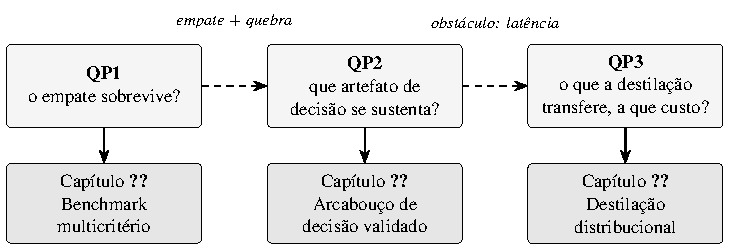
\includegraphics{images/tikz-cap1-1.pdf}
\caption{Perguntas de pesquisa e capítulos que as respondem.}
\label{fig:intro-qps}
\end{figure}

\section{Resumo das contribuições}
\label{sec:intro-contribuicoes}

As contribuições desta dissertação são de \emph{medição sob protocolo
uniforme} e de \emph{validação honesta} --- não se reivindica mecanismo
novo de aprendizado; reivindica-se, com verificações de novidade datadas,
o recorte e a evidência que faltavam. Em ordem de apresentação:

\begin{enumerate}
  \item \textbf{Um benchmark multicritério da era dos foundation models}
    --- 14 modelos $\times$ 18 conjuntos (250 das 252 células; duas
    exclusões estruturais declaradas), com validação cruzada aninhada,
    inferência frequentista e bayesiana e três eixos de custo sob o mesmo
    protocolo. Dele saem os dois fatos que estruturam a dissertação: o
    empate estatístico da geração anterior (8 de 10 modelos praticamente
    equivalentes ao líder; 80\% da variância de rank intrafamília) e a
    quebra do empate pela geração 2026 (TabFM líder nas três tarefas e
    melhor modelo em 13 de 18 conjuntos, \emph{zero-shot}, ao preço de
    quatro a cinco ordens de magnitude em latência). Inclui a primeira
    comparação neutra TabPFN~$\times$~TabFM sob protocolo idêntico, até
    onde alcançam as verificações datadas (Capítulo~\ref{chap:benchmark}).
  \item \textbf{Um resultado negativo independente sobre as redes de
    Kolmogorov--Arnold} --- no primeiro teste da família contra a grade
    completa GBDT/aprendizado profundo/\emph{foundation models} em
    benchmark multicritério (verificação datada), KAN e TabKAN terminam no
    último terço nas três tarefas, embora baratas de servir: sob protocolo
    uniforme com ajuste equalizado, as alegações dos artigos originais não
    se sustentam (Capítulo~\ref{chap:benchmark}).
  \item \textbf{Um arcabouço de decisão validado, não apenas descrito} ---
    três estudos sob \emph{leave-one-dataset-out} elevam o fluxograma de
    decisão de descritivo a validado: o roteamento por meta-características
    não generaliza (taxa de acerto 0,11 contra 0,44 do \emph{baseline}
    trivial no estudo com 11 modelos; 0,72 contra 0,78 com 14); a política
    fixa ``\emph{foundation model} primeiro'' é \emph{regret}-ótima na
    métrica primária, com \emph{regret} mediano zero na geração 2026; e o
    experimento pré-registrado E2, contribuição exclusiva desta
    dissertação, localiza o ponto de inversão --- basta deslocar 10 a 20\%
    do peso da acurácia para a latência para a recomendação virar ---,
    justificando quantitativamente a arquitetura do fluxograma
    (Capítulo~\ref{chap:framework}).
  \item \textbf{A destilação distribucional de foundation models
    tabulares} --- o recorte verificado como inédito: sob desenho
    pré-registrado em 20 conjuntos, a destilação \emph{pontual} falha de
    forma robusta com qualquer professor (um resultado negativo reportado
    com proeminência integral), enquanto a transferência das curvas de
    quantis retém mediana de 19\% da vantagem distribucional do professor,
    positiva em 16 de 20 conjuntos (teste de sinal $p=0{,}006$), a
    latências de microssegundos; a primeira fronteira medida de ponta a
    ponta entre destilar, comprimir contexto e reduzir \emph{ensemble}; a
    ablação que mostra que a rotulagem \emph{out-of-fold} protege
    calibração, não acurácia; o experimento pré-registrado E1, também
    exclusivo desta dissertação, em que o aluno destilado vence
    \emph{baselines} distribucionais clássicos em 17 de 20 conjuntos
    ($p=0{,}0013$); e a regra de decisão prática que converte as
    refutações em instrução verificável em minutos
    (Capítulo~\ref{chap:destilacao}).
  \item \textbf{Infraestrutura e conduta reutilizáveis} --- o protocolo, os
    artefatos versionados (cada número do texto rastreia a um CSV,
    JSON ou notebook executado), os pré-registros com adendos datados, as
    verificações de novidade registradas e o rito de errata pública
    constituem, em conjunto, uma contribuição metodológica de
    reprodutibilidade, descrita no Capítulo~\ref{chap:metodologia} e
    exercitada ao longo de toda a parte empírica.
\end{enumerate}

\section{Produção bibliográfica}
\label{sec:intro-producao}

A pesquisa gerou, até o depósito desta dissertação, dois relatórios
técnicos do programa de pós-graduação, correspondentes às disciplinas de
trabalho individual, ambos em inglês e disponíveis no repositório público
do projeto:

\begin{itemize}
  \item \textbf{AI-1} --- \emph{Does ``GBDT Always Win''? A Multi-Criteria
    Benchmark of 14 Tabular Models --- From a Statistical Tie to the 2026
    Break --- and a Validated Decision Framework} \citep{companion2026}:
    relatório técnico do Trabalho Individual (\texttt{latex/ai1/} no
    repositório), que condensa o material dos
    Capítulos~\ref{chap:benchmark} e~\ref{chap:framework}.
  \item \textbf{AI-2} --- \emph{Distilling Tabular Foundation Models
    Beyond Classification: Distributional Regression and the
    Distill/Compress/Shrink Pareto Frontier} \citep{companion-ai2-2026}: relatório técnico da Atividade de
    Orientação Individual (\texttt{latex/ai2/}), que condensa o material
    do Capítulo~\ref{chap:destilacao}; um preprint derivado dele está em
    preparação para submissão ao arXiv.
\end{itemize}

Os dois relatórios são trabalhos avaliativos do programa, sem revisão por
pares externa até a data desta escrita; seu conteúdo corresponde,
respectivamente, aos Capítulos~\ref{chap:benchmark}
e~\ref{chap:framework} e ao Capítulo~\ref{chap:destilacao}, que incluem
ainda os dois experimentos (E1 e E2) que são contribuições novas da
dissertação, inéditas em relação aos relatórios.

\section{Como ler esta dissertação}
\label{sec:intro-comoler}

A dissertação foi escrita para três perfis de leitor, e nem todos precisam
percorrê-la linearmente. O \textbf{praticante} --- quem precisa escolher e
servir um modelo tabular --- pode ir diretamente aos
Capítulos~\ref{chap:benchmark} e~\ref{chap:framework} (a evidência e o
fluxograma de decisão) e à regra de decisão que encerra o
Capítulo~\ref{chap:destilacao} (Seção~\ref{sec:destil-regra}): os três
pontos foram escritos para serem autocontidos, com os pré-requisitos
mínimos recapitulados no início de cada capítulo. O \textbf{leitor de
formação estatística} interessado no rigor das comparações deve começar
pela Seção~\ref{sec:fund-estatistica} do Capítulo~\ref{chap:fundamentacao}
(a teoria dos testes, incluindo a camada bayesiana de equivalência
prática) e pelo Capítulo~\ref{chap:metodologia} (o protocolo de aplicação,
a política para células faltantes e as limitações declaradas antes dos
resultados). O \textbf{replicador} --- quem quer reproduzir ou estender os
experimentos --- encontra no Capítulo~\ref{chap:metodologia} o protocolo
completo com sementes, versões e justificativas, e nos apêndices o
restante: as tabelas completas por conjunto
(Apêndice~\ref{app:tabelas}), os espaços de busca de hiperparâmetros
(Apêndice~\ref{app:espacos-busca}) e os resultados suplementares e
ablações; todos os artefatos citados têm caminho explícito no repositório
público do projeto.

\section{Estrutura da dissertação}
\label{sec:intro-estrutura}

O restante da dissertação está organizado em sete capítulos e três
apêndices. O \textbf{Capítulo~\ref{chap:fundamentacao}} constrói, do
concreto ao abstrato, o vocabulário técnico do trabalho: dados tabulares e
sua heterogeneidade constitutiva, árvores e \emph{gradient boosting}, as
três linhagens do aprendizado profundo tabular, os \emph{foundation
models} e o mecanismo de aprendizado em contexto, a destilação de
conhecimento, o ferramental da regressão distribucional (quantis, CRPS,
calibração) e a teoria dos testes estatísticos para comparação de
algoritmos --- com profundidade matemática proporcional à proximidade das
contribuições. O \textbf{Capítulo~\ref{chap:related}} posiciona o trabalho
em seis eixos da literatura, de benchmarks tabulares à destilação de
\emph{foundation models}, fechando com uma tabela-síntese que liga cada
lacuna --- caracterizada por verificações online datadas --- ao capítulo
que a ataca. O \textbf{Capítulo~\ref{chap:metodologia}} especifica o
protocolo experimental comum a toda a parte empírica: conjuntos, modelos,
validação cruzada aninhada com \emph{hold-out} intocado, métricas,
protocolo de inferência estatística, medição de custo, infraestrutura de
reprodutibilidade e o contrato de conduta científica, com as limitações do
desenho declaradas antes de qualquer resultado. O
\textbf{Capítulo~\ref{chap:benchmark}} apresenta o benchmark em quatro
atos --- o empate estatístico do núcleo de 11 modelos, os eixos de custo
em que os empatados diferem por ordens de magnitude, as reversões
condicionais e o eixo do tamanho amostral, e a quebra do empate pela
geração 2026, com o resultado negativo das redes de Kolmogorov--Arnold ---
respondendo à QP1. O \textbf{Capítulo~\ref{chap:framework}} eleva o
arcabouço de decisão de descritivo a validado por três estudos sob
\emph{leave-one-dataset-out} --- o resultado negativo do roteamento por
meta-características, o positivo da política ``\emph{foundation model}
primeiro'' e o experimento pré-registrado de \emph{regret} multicritério
ponderado --- consolidando o fluxograma de quatro restrições que responde
à QP2. O \textbf{Capítulo~\ref{chap:destilacao}} apresenta a contribuição
de destilação distribucional sob desenho pré-registrado: a refutação da
destilação pontual, o sucesso da transferência de curvas de quantis, a
fronteira de três estratégias de serviço, a ablação da rotulagem
\emph{out-of-fold}, o experimento E1 contra \emph{baselines} clássicos e a
regra de decisão final que responde à QP3. O
\textbf{Capítulo~\ref{chap:conclusao}} confronta cada pergunta de pesquisa
com a evidência acumulada, consolida as contribuições, declara as
limitações e ameaças à validade do programa como um todo e aponta os
trabalhos futuros. Os \textbf{apêndices} reúnem as tabelas completas de
resultados por conjunto, os espaços de busca de hiperparâmetros e os
resultados suplementares e ablações.

\chapter{Fundamentação Teórica}
\label{chap:fundamentacao}

\begin{resumocapitulo}
Este capítulo constrói, do concreto ao abstrato, todo o vocabulário técnico
de que a dissertação precisa: o que são dados tabulares e por que eles
resistem às arquiteturas que revolucionaram visão e linguagem
(\S\ref{sec:fund-tabular}); como uma única árvore de decisão aprende e por
que \emph{ensembles} de árvores com \emph{boosting} se tornaram o padrão da
área (\S\ref{sec:fund-gbdt}); as três linhagens da resposta do aprendizado
profundo, do MLP aos Transformers e às redes de Kolmogorov--Arnold
(\S\ref{sec:fund-dl}); os \emph{foundation models} tabulares e o mecanismo
de aprendizado em contexto que dispensa treinamento na tarefa
(\S\ref{sec:fund-fm}); a destilação de conhecimento
(\S\ref{sec:fund-destilacao}); o ferramental da regressão distribucional
--- perda \emph{pinball}, CRPS, calibração --- que sustenta a contribuição
do Capítulo~7 (\S\ref{sec:fund-distribucional}); e os testes estatísticos
com que o Capítulo~5 compara os modelos (\S\ref{sec:fund-estatistica}). A
profundidade matemática cresce com a proximidade das contribuições: o
\emph{boosting} é apresentado verbalmente, a atenção com suas equações
completas, e a regressão distribucional e a inferência estatística com o
detalhe necessário para ler os resultados sem consultar as fontes.
\end{resumocapitulo}

\publicacaoassociada{As formulações de CRPS, PICP, perda \emph{pinball} e
aprendizado em contexto das Seções~\ref{sec:fund-fm}
e~\ref{sec:fund-distribucional} seguem as glosas auditadas dos dois artigos
que acompanham esta dissertação (\texttt{latex/ai1} e \texttt{latex/ai2} no
repositório), aqui traduzidas e expandidas didaticamente.}

\paragraph{Roteiro.} O leitor já familiarizado com \emph{gradient boosting}
e redes neurais pode saltar diretamente para a
Seção~\ref{sec:fund-fm}, onde começa o material menos difundido
(aprendizado em contexto e cabeças distribucionais); quem conhece os
\emph{foundation models} tabulares, para as
Seções~\ref{sec:fund-distribucional} e~\ref{sec:fund-estatistica}, que são
pré-requisito direto dos Capítulos~5 e~7. As demais seções foram escritas
para que um leitor com formação geral em computação acompanhe toda a
dissertação sem fontes externas.

\section{Dados tabulares e aprendizagem supervisionada}
\label{sec:fund-tabular}

Comecemos pelo objeto. Um \emph{conjunto de dados tabular} é uma tabela em
que cada linha é uma observação e cada coluna um atributo --- o formato de
um extrato bancário, de um prontuário ou de um cadastro de clientes. A
Tabela~\ref{tab:adult-exemplo} ilustra o formato com linhas no estilo do
conjunto \texttt{adult}, um clássico da área em que se deseja prever, a
partir de atributos sociodemográficos de um censo, se a renda anual de uma
pessoa excede 50 mil dólares \textbf{[REF-NOVA: Kohavi 1996, conjunto
Adult/Census Income do repositório UCI]}.

\begin{table}[htb]
\centering
\caption{Fragmento \emph{ilustrativo} de um conjunto tabular no estilo do
\texttt{adult}. As linhas são fictícias, porém plausíveis; servem apenas
para fixar o formato: atributos numéricos e categóricos convivem na mesma
tabela, há valores ausentes (``?'') e a última coluna é o alvo a prever.}
\label{tab:adult-exemplo}
\begin{tabular}{rllrl}
\toprule
idade & escolaridade & ocupação & horas/semana & renda $>$ 50K? \\
\midrule
39 & superior        & gerência        & 45 & sim \\
23 & ensino médio    & serviços        & 40 & não \\
51 & pós-graduação   & especialista    & 50 & sim \\
34 & ensino médio    & ?               & 38 & não \\
28 & superior        & técnico         & 44 & não \\
\bottomrule
\end{tabular}
\end{table}

\paragraph{A heterogeneidade é constitutiva.} A Tabela~\ref{tab:adult-exemplo}
já exibe tudo o que torna o formato difícil: \texttt{idade} e
\texttt{horas/semana} são números em escalas distintas;
\texttt{escolaridade} é uma categoria com ordem natural;
\texttt{ocupação} é uma categoria \emph{nominal}, sem ordem nem distância
entre valores, e de cardinalidade arbitrária; e o ``?'' é um valor ausente
cuja ausência pode, ela própria, carregar informação. Uma mesma tabela
mistura, portanto, variáveis contínuas, contagens, categorias e lacunas ---
e cada coluna é um eixo semântico independente: trocar duas colunas de
lugar não altera o problema, mas trocar dois pixels de uma imagem, sim.

\paragraph{Por que as revoluções de visão e linguagem não transferiram?}
Redes convolucionais exploram a estrutura espacial das imagens (pixels
vizinhos são correlacionados; padrões se repetem em qualquer posição);
Transformers de linguagem exploram a estrutura sequencial do texto. Dados
tabulares não oferecem nenhuma invariância universal análoga que uma
arquitetura possa explorar \emph{por construção} --- não há noção de
vizinhança entre \texttt{idade} e \texttt{ocupação}. Essa ausência de
estrutura compartilhada é a explicação usual para um fato empírico
persistente: por mais de uma década, o estado da arte em tabelas pertenceu
a outra família de modelos, os \emph{ensembles} de árvores de decisão
\citep{grinsztajn2022,mcelfresh2023}. As Seções~\ref{sec:fund-gbdt}
e~\ref{sec:fund-dl} desenvolvem os dois lados dessa disputa.

\paragraph{O problema da aprendizagem supervisionada.} Formalizemos o
mínimo necessário. Dado um conjunto de treino
$D = \{(\mathbf{x}_i, y_i)\}_{i=1}^{n}$ de pares observação--alvo,
assumidos amostras independentes de uma distribuição desconhecida, o
objetivo é aprender uma função $f$ que prediga bem o alvo de observações
\emph{novas} --- isto é, que minimize o erro esperado sob a distribuição
geradora, não o erro no próprio conjunto de treino. A distinção é o coração
do problema: um modelo suficientemente flexível pode zerar o erro de treino
simplesmente memorizando $D$ (\emph{sobreajuste}), sem generalizar. Por
isso toda avaliação honesta mede o desempenho em dados que o modelo --- e,
igualmente importante, o processo de \emph{escolha} do modelo --- jamais
viu; o Capítulo~4 traduz esse princípio em protocolo (conjunto de teste
separado antes de tudo, validação cruzada aninhada para a seleção de
hiperparâmetros).

\paragraph{As três tarefas.} Este trabalho considera os três tipos
canônicos de tarefa supervisionada sobre tabelas: \emph{classificação
binária} (prever uma de duas classes, como na
Tabela~\ref{tab:adult-exemplo}), \emph{classificação multiclasse} (prever
uma entre $K$ classes) e \emph{regressão} (prever um valor contínuo). A
regressão admite duas leituras que esta dissertação distingue com cuidado:
a leitura \emph{pontual}, em que o modelo devolve um único número (uma
estimativa da média condicional), e a leitura \emph{distribucional}, em que
o modelo devolve uma distribuição preditiva completa --- quantis,
intervalos, densidades --- da qual se exige calibração. A distinção parece
sutil agora, mas é o eixo da contribuição do Capítulo~7, e a
Seção~\ref{sec:fund-distribucional} lhe dedica o ferramental próprio.

\section{Das árvores de decisão ao \emph{gradient boosting}}
\label{sec:fund-gbdt}

\subsection{Uma árvore, um exemplo guiado}

Uma \emph{árvore de decisão} prediz por meio de uma sequência de perguntas
sobre os atributos, cada uma com resposta binária, até chegar a uma folha
que contém a predição \textbf{[REF-NOVA: Breiman, Friedman, Olshen \& Stone
1984, CART]}. A Figura~\ref{fig:arvore-exemplo} mostra uma árvore pequena,
de profundidade dois, treinada (ilustrativamente) sobre dados como os da
Tabela~\ref{tab:adult-exemplo}.

\begin{figure}[htb]
\centering
\begin{tikzpicture}[
  level distance=17mm,
  level 1/.style={sibling distance=62mm},
  level 2/.style={sibling distance=31mm},
  interno/.style={draw, rounded corners=2pt, align=center, font=\small,
                  inner sep=4pt},
  folha/.style={draw, rounded corners=2pt, align=center, font=\small,
                fill=black!6, inner sep=4pt},
  rotulo/.style={font=\footnotesize\itshape, midway},
  edge from parent/.style={draw, -{Stealth[length=2mm]}}]
\node[interno] {escolaridade $\geq$ superior?}
  child { node[interno] {horas/semana $>$ 45?}
    child { node[folha] {$\hat{p} = 0{,}06$}
      edge from parent node[rotulo, left=1pt] {não} }
    child { node[folha] {$\hat{p} = 0{,}22$}
      edge from parent node[rotulo, right=1pt] {sim} }
    edge from parent node[rotulo, left=3pt] {não} }
  child { node[interno] {idade $>$ 30?}
    child { node[folha] {$\hat{p} = 0{,}29$}
      edge from parent node[rotulo, left=1pt] {não} }
    child { node[folha] {$\hat{p} = 0{,}61$}
      edge from parent node[rotulo, right=1pt] {sim} }
    edge from parent node[rotulo, right=3pt] {sim} };
\end{tikzpicture}
\caption{\textbf{Uma árvore de decisão responde por partições sucessivas do
espaço de atributos.} Árvore ilustrativa de profundidade 2 sobre o exemplo
da Tabela~\ref{tab:adult-exemplo}; em cada folha, $\hat{p}$ é a fração de
exemplos de treino daquela região com renda $>$ 50K (valores fictícios,
para ilustração). Para classificar uma linha nova, percorre-se o caminho
ditado pelas respostas e lê-se a predição na folha alcançada.}
\label{fig:arvore-exemplo}
\end{figure}

Siga a terceira linha da Tabela~\ref{tab:adult-exemplo} pela árvore: a
pessoa tem pós-graduação (escolaridade $\geq$ superior: \emph{sim}, ramo
direito) e 51 anos (idade $>$ 30: \emph{sim}), caindo na folha com
$\hat{p} = 0{,}61$ --- a árvore estima 61\% de probabilidade de renda alta,
e, com limiar de 50\%, prediz ``sim''. O treinamento constrói essas
perguntas de cima para baixo, escolhendo em cada nó, por busca gulosa, o
atributo e o ponto de corte que melhor separam as classes (segundo um
critério de impureza como entropia ou índice de Gini); em regressão, as
folhas guardam médias e o critério é a redução de variância.

Duas propriedades dessa construção merecem registro desde já, porque
reaparecerão como explicação de resultados empíricos. Primeiro, as
partições são \emph{alinhadas aos eixos}: cada pergunta envolve um único
atributo, o que casa com a natureza tabular em que cada coluna tem
semântica própria. Segundo, a árvore é \emph{invariante a transformações
monótonas} de cada atributo --- perguntar ``idade $>$ 30'' é equivalente a
perguntar ``$\log(\text{idade}) > \log 30$'' --- de modo que normalizar
colunas, etapa obrigatória para redes neurais, é irrelevante para árvores.

\subsection{Por que uma árvore só não basta?}

Uma árvore única enfrenta um dilema. Se for rasa, é estável porém grosseira:
o exemplo da Figura~\ref{fig:arvore-exemplo} reduz toda a população a
quatro grupos. Se for profunda, torna-se expressiva porém instável:
memoriza particularidades da amostra de treino, e uma pequena perturbação
nos dados produz uma árvore muito diferente. Na linguagem clássica da
decomposição \emph{viés--variância}, árvores rasas sofrem de viés alto e
árvores profundas, de variância alta \textbf{[REF-NOVA: Hastie, Tibshirani
\& Friedman 2009, \emph{The Elements of Statistical Learning}]}. Os
\emph{ensembles} --- comitês de árvores --- atacam cada chifre do dilema
por um caminho distinto.

\paragraph{Caminho 1: reduzir a variância em paralelo.} O \emph{bagging} e
seu refinamento mais célebre, as florestas aleatórias, treinam muitas
árvores profundas em réplicas perturbadas dos dados (reamostragem com
reposição e sorteio de atributos por nó) e tiram a média das predições: os
erros idiossincráticos de cada árvore, aproximadamente independentes,
cancelam-se na média, e a variância do comitê despenca sem elevar o viés
\textbf{[REF-NOVA: Breiman 2001, \emph{Random Forests}]}.

\paragraph{Caminho 2: reduzir o viés em sequência.} O \emph{boosting}
inverte a lógica: parte de árvores \emph{rasas} (viés alto, variância
baixa) e as treina em sequência, cada nova árvore concentrada em corrigir
os erros que o comitê acumulado ainda comete. A predição final é a soma
ponderada de todas as correções. A cada rodada, os exemplos mal preditos
ganham protagonismo, e o comitê refina exatamente as regiões em que ainda
erra --- o viés cai passo a passo, enquanto a rasura de cada árvore e um
passo de aprendizado pequeno seguram a
variância.\footnote{Tecnicamente, o \emph{gradient boosting} formaliza essa
intuição como uma descida de gradiente no espaço de funções: a cada rodada
$m$, ajusta-se uma árvore $h_m$ ao gradiente negativo da função de perda
avaliada nas predições correntes (no caso do erro quadrático, aos resíduos
$y_i - F_{m-1}(x_i)$), e atualiza-se $F_m = F_{m-1} + \nu\, h_m$ com taxa
de aprendizado $\nu$ pequena \textbf{[REF-NOVA: Friedman 2001,
\emph{Greedy Function Approximation: A Gradient Boosting Machine}]}. O
corpo do texto permanece verbal de propósito: nenhum resultado desta
dissertação exige manipular essa formulação.}

\subsection{XGBoost, LightGBM e CatBoost: uma diferença concreta cada}

Três implementações modernas de \emph{gradient boosting} sobre árvores
(GBDTs, de \emph{gradient-boosted decision trees}) dominam a prática, e o
benchmark do Capítulo~5 avalia as três. Para os fins desta dissertação,
basta reter uma diferença concreta de cada uma. O \textbf{XGBoost}
\citep{chen2016} consolidou o paradigma com uma formulação regularizada do
objetivo --- penalidades explícitas sobre o número de folhas e a magnitude
dos pesos --- que disciplina o crescimento de cada árvore. O
\textbf{LightGBM} \citep{ke2017} muda a ordem de crescimento: em vez de
expandir a árvore nível a nível, expande sempre a \emph{folha} de maior
ganho (crescimento folha-a-folha), com histogramas de atributos que tornam
o treino substancialmente mais rápido em dados grandes. O
\textbf{CatBoost} \citep{prokhorenkova2018} distingue-se pelo tratamento
nativo de variáveis categóricas via \emph{ordered boosting}: as estatísticas
de alvo usadas para codificar categorias são computadas apenas sobre
exemplos ``anteriores'' numa permutação aleatória, evitando o vazamento de
alvo das codificações ingênuas.

\paragraph{Os botões de ajuste.} Na prática, o comportamento de um GBDT é
governado por um punhado de hiperparâmetros com papéis interpretáveis à luz
do dilema viés--variância: a \emph{profundidade} das árvores controla a
ordem das interações que cada correção pode capturar; o \emph{número de
árvores} e a \emph{taxa de aprendizado} formam um par acoplado (passos
menores exigem mais passos, mas regularizam); e as frações de
\emph{subamostragem} de linhas e colunas por árvore injetam a
descorrelação que o \emph{bagging} ensinou. Nenhuma configuração domina
todos os conjuntos de dados --- razão pela qual qualquer comparação justa
entre modelos precisa otimizar os hiperparâmetros de cada um sob o mesmo
orçamento, como especifica o Capítulo~4.

\paragraph{Por que o \emph{boosting} domina dados tabulares?} Reunindo os
fios: as partições alinhadas aos eixos capturam não-linearidades e
interações por atributo sem supor qualquer geometria entre colunas; a
invariância a transformações monótonas dispensa normalização e absorve
escalas heterogêneas; a seleção gulosa de cortes ignora com naturalidade
atributos irrelevantes; e o \emph{boosting} compõe essas virtudes num
redutor sistemático de viés. O resultado é um desempenho consistente, com
pouco ajuste, exatamente no regime de dados heterogêneos de tamanho pequeno
a médio --- diagnóstico corroborado por avaliações independentes em larga
escala \citep{grinsztajn2022,mcelfresh2023}. Por isso, nesta dissertação os
GBDTs cumprem o papel de \emph{hipótese nula}: toda proposta nova em dados
tabulares deve ser medida contra eles.

\section{Aprendizado profundo para dados tabulares}
\label{sec:fund-dl}

A resposta do aprendizado profundo ao domínio dos GBDTs organizou-se em
três linhagens: modernizar o MLP, importar a atenção dos Transformers e,
mais recentemente, repensar o próprio neurônio com as redes de
Kolmogorov--Arnold. Esta seção as percorre em ordem.

\subsection{O perceptron multicamadas}

O \emph{perceptron multicamadas} (MLP) é a rede neural mais simples:
camadas de unidades que combinam linearmente as entradas e aplicam uma
não-linearidade. Com entrada $\mathbf{h}^{(0)} = \mathbf{x}$, cada camada
$l$ computa
\begin{equation}
  \mathbf{h}^{(l)} \;=\; \phi\!\left(\mathbf{W}^{(l)} \mathbf{h}^{(l-1)}
  + \mathbf{b}^{(l)}\right),
  \label{eq:mlp-camada}
\end{equation}
em que $\mathbf{W}^{(l)}$ e $\mathbf{b}^{(l)}$ são parâmetros aprendidos e
$\phi$ é uma função de ativação fixa (tipicamente a ReLU,
$\phi(z) = \max(0, z)$), e a saída da última camada é lida como predição,
\begin{equation}
  f(\mathbf{x}) \;=\; \mathbf{W}^{(L)} \mathbf{h}^{(L-1)} + \mathbf{b}^{(L)},
  \label{eq:mlp-saida}
\end{equation}
seguida de uma \emph{softmax} em classificação. Os parâmetros são ajustados
por descida de gradiente sobre uma função de perda, com gradientes
computados por retropropagação \textbf{[REF-NOVA: Rumelhart, Hinton \&
Williams 1986, retropropagação]}. Em uma frase: com largura suficiente, um
MLP pode aproximar qualquer função contínua \textbf{[REF-NOVA: Hornik,
Stinchcombe \& White 1989, aproximação universal]} --- a questão em dados
tabulares nunca foi expressividade, e sim se o treinamento encontra, com
dados finitos e heterogêneos, soluções tão boas quanto as dos GBDTs.

\paragraph{O gargalo do encoding categórico.} Antes de qualquer camada, há
uma decisão incômoda: como entregar \texttt{ocupação} a uma rede que só
consome números? A codificação \emph{one-hot} --- uma coluna binária por
categoria --- explode a dimensionalidade quando a cardinalidade é alta: no
benchmark desta dissertação, o conjunto \texttt{amazon\_employee} atingiria
cerca de 6{,}9 mil colunas sem um teto de cardinalidade, penalizando
especialmente os modelos de atenção, cujo custo cresce com o número de
colunas. A alternativa padrão são \emph{embeddings} aprendidos: cada
categoria é mapeada a um vetor denso de baixa dimensão, treinado junto com
a rede --- solução que todas as arquiteturas a seguir adotam de alguma
forma.

\paragraph{A receita importa: RealMLP e TabM.} Duas propostas recentes
mostram que boa parte da desvantagem histórica do MLP era de \emph{receita},
não de arquitetura. O \textbf{RealMLP} \citep{realmlp2024} demonstra que um
MLP com um conjunto cuidadoso de melhorias --- \emph{embeddings} numéricos,
agendamento de taxa de aprendizado, regularização e pré-processamento
afinados --- compete com GBDTs ajustados. O \textbf{TabM} \citep{tabm2025}
ataca outro flanco: obtém o efeito estabilizador de um \emph{ensemble} de
MLPs com custo próximo ao de um modelo único, parametrizando eficientemente
múltiplas ``sub-redes'' que compartilham a maior parte dos pesos.

\paragraph{Por que insistir em redes para tabelas?} Se os GBDTs dominam,
por que a área continua investindo em redes? Por três promessas que
árvores não fazem. Primeiro, redes aprendem \emph{representações}:
\emph{embeddings} de categorias e camadas intermediárias reutilizáveis,
porta de entrada para transferência entre tarefas e para dados mistos
(tabela junto a texto ou imagem). Segundo, redes são treináveis por
gradiente de \emph{qualquer} perda diferenciável, o que permite cabeças de
saída flexíveis --- multi-alvo, multi-quantil, distribucionais --- com
mudança mínima de arquitetura; essa plasticidade é explorada diretamente
pelos alunos de destilação do Capítulo~7. Terceiro, e decisivo para esta
dissertação: toda a família de \emph{foundation models} da
Seção~\ref{sec:fund-fm}, que redefine o custo de entrada em novas tarefas,
só é possível sobre redes.

\subsection{Atenção e Transformers}

A segunda linhagem importa o mecanismo que revolucionou o processamento de
linguagem: a \emph{atenção} \textbf{[REF-NOVA: Vaswani et al. 2017,
\emph{Attention Is All You Need}]}. Aqui a profundidade matemática se
justifica: metade dos modelos do benchmark e todos os \emph{foundation
models} da Seção~\ref{sec:fund-fm} são construídos sobre essas equações.

Dada uma sequência de $n$ vetores de entrada empilhados em
$\mathbf{X} \in \mathbb{R}^{n \times d}$, a atenção projeta cada vetor em
três papéis --- \emph{consulta} (\emph{query}), \emph{chave} (\emph{key}) e
\emph{valor} (\emph{value}):
\begin{equation}
  \mathbf{Q} = \mathbf{X}\mathbf{W}_Q, \qquad
  \mathbf{K} = \mathbf{X}\mathbf{W}_K, \qquad
  \mathbf{V} = \mathbf{X}\mathbf{W}_V,
  \label{eq:qkv}
\end{equation}
com matrizes de projeção aprendidas, e produz, para cada posição, uma média
dos valores ponderada pela afinidade entre sua consulta e todas as chaves:
\begin{equation}
  \operatorname{Atenção}(\mathbf{Q}, \mathbf{K}, \mathbf{V})
  \;=\; \operatorname{softmax}\!\left(
    \frac{\mathbf{Q}\mathbf{K}^{\top}}{\sqrt{d_k}}
  \right)\mathbf{V},
  \label{eq:atencao}
\end{equation}
em que $d_k$ é a dimensão das chaves e a divisão por $\sqrt{d_k}$ estabiliza
as magnitudes antes da \emph{softmax}. A intuição: cada elemento da
sequência ``pergunta'' (via $\mathbf{Q}$) quais outros elementos lhe são
relevantes (via $\mathbf{K}$) e agrega a informação deles (via $\mathbf{V}$)
na proporção dessa relevância --- pesos que são \emph{computados dos
dados}, não fixados pela arquitetura. A atenção \emph{multi-cabeça} executa
$h$ atenções em paralelo com projeções independentes e concatena os
resultados,
\begin{equation}
  \operatorname{MultiHead}(\mathbf{X}) \;=\;
  \operatorname{concat}(\text{cabeça}_1, \ldots, \text{cabeça}_h)\,
  \mathbf{W}_O,
  \label{eq:multihead}
\end{equation}
permitindo que cabeças distintas capturem padrões de interação distintos. Um
\emph{bloco Transformer} empilha atenção multi-cabeça e um MLP
posição-a-posição, com conexões residuais e normalização de camada; a
arquitetura completa original empilha esses blocos em um \emph{encoder}
(que processa a entrada inteira de uma vez, com atenção irrestrita) e um
\emph{decoder} (que gera texto token a token, com atenção causal).

\paragraph{Por que dados tabulares usam só o \emph{encoder}?} Porque não há
nada a \emph{gerar} sequencialmente: a predição sobre uma linha é um único
rótulo ou valor, não uma sequência. Os Transformers tabulares tratam as
\emph{colunas} de uma linha como a ``sequência'' de entrada --- cada
atributo vira um token --- e usam apenas a pilha de \emph{encoder}: a
atenção entre tokens-atributo aprende interações entre colunas, e a
predição é lida de um token especial agregador. O \emph{decoder} e sua
máscara causal, feitos para a ordem temporal do texto, não têm contraparte
numa linha de tabela.

\paragraph{As arquiteturas de atenção do benchmark.} O \textbf{TabNet}
\citep{arik2021} foi pioneiro em levar atenção a tabelas, combinando-a com
seleção \emph{esparsa} de atributos: a cada passo de processamento, uma
máscara aprendida elege poucos atributos relevantes, o que confere ao
modelo interpretabilidade nativa. O \textbf{FT-Transformer}
\citep{gorishniy2021} é a destilação mais limpa da ideia: um
\emph{Feature Tokenizer} converte cada atributo (numérico ou categórico) em
um token-\emph{embedding} e um Transformer padrão processa a linha; é a
referência arquitetural da linhagem. O \textbf{SAINT} \citep{somepalli2021}
acrescenta à atenção entre colunas uma atenção \emph{entre linhas}
(\emph{intersample}): ao classificar uma linha, o modelo pode consultar
outras linhas do lote --- um antecipo, em miniatura, da ideia de usar
exemplos como contexto que a Seção~\ref{sec:fund-fm} leva ao extremo. O
\textbf{STab} \citep{stab-ref} completa a linhagem no benchmark
[VERIFICAR: descrição do STab --- o rascunho-fonte (\texttt{dissertation/}\allowbreak\texttt{cap2-fundamentacao.md}) o descreve como competição estocástica local
(LWTA) de Voskou et al., mas a entrada \texttt{stab-ref} do
\texttt{references.bib} aponta para Hajiramezanali et al. 2022,
aprendizado autossupervisionado para tabelas; conferir qual STab foi
implementado e alinhar descrição e referência].

\subsection{Redes de Kolmogorov--Arnold}

A terceira linhagem, mais recente, muda o lugar da não-linearidade. O
teorema da representação de Kolmogorov--Arnold garante que toda função
contínua de várias variáveis pode ser escrita como composição de somas de
funções contínuas de \emph{uma} variável \textbf{[REF-NOVA: Kolmogorov 1957
e Arnold, teorema da representação]}. As \emph{Kolmogorov--Arnold Networks}
(KANs) \citep{kan2024} tomam o teorema como inspiração arquitetural e
invertem o desenho do MLP: em vez de ativações fixas nos nós e pesos
escalares nas arestas (Eq.~\ref{eq:mlp-camada}), colocam \emph{funções
univariadas aprendíveis} nas arestas --- parametrizadas por B-splines ---
e meras somas nos nós. Cada conexão deixa de ser um número e passa a ser
uma pequena curva ajustável. Variantes trocam a base das funções de aresta
(polinômios de Chebyshev no ChebyKAN, funções de base radial no FastKAN), e
o \textbf{TabKAN} \citep{tabkan2025} organiza essas variantes num arcabouço
voltado a dados tabulares.

\paragraph{Uma recepção controversa.} A promessa das KANs --- mais
expressividade por parâmetro e interpretabilidade das curvas aprendidas ---
encontrou ceticismo empírico: sob comparação com paridade de parâmetros e
de FLOPs, o MLP vence as KANs na maioria das tarefas de aprendizado de
máquina \citep{kancritical2024}, e avaliações independentes em tabelas
chegaram a quadro semelhante \citep{poeta2024}. Nenhuma dessas avaliações,
porém, inclui GBDTs e \emph{foundation models} no mesmo protocolo --- a
lacuna que o Capítulo~5 preenche, adjudicando a controvérsia sob protocolo
neutro.

\section{\emph{Foundation models} tabulares e aprendizado em contexto}
\label{sec:fund-fm}

Tudo o que foi visto até aqui compartilha uma premissa tão básica que passa
despercebida: para cada novo conjunto de dados, treina-se um modelo novo.
Os \emph{foundation models} tabulares abandonam essa premissa, e é
essencial entender o mecanismo --- não apenas o efeito --- porque tanto o
custo de inferência medido no Capítulo~5 quanto a destilação do Capítulo~7
decorrem diretamente dele.

\paragraph{O mecanismo: treinar virou condicionar.} Um modelo de
\emph{aprendizado em contexto} (\emph{in-context learning}, ICL) é uma rede
pré-treinada que condiciona no conjunto de treino como se fosse um
\emph{prompt}, no momento da predição, sem nenhuma atualização de gradiente
na tarefa-alvo. Concretamente: apresenta-se ao Transformer, numa única
entrada, o conjunto de treino inteiro --- pares $(\mathbf{x}_i, y_i)$ ---
seguido da linha de consulta $\mathbf{x}_{\text{novo}}$; um único passe
direto (\emph{forward pass}) produz a predição, com os pesos da rede
congelados. ``Treinar'' na tarefa reduz-se a montar o contexto; todo o
aprendizado propriamente dito aconteceu antes, no pré-treinamento. A
Figura~\ref{fig:icl-mecanismo} esquematiza as duas fases.

\begin{figure}[htb]
\centering
\begin{tikzpicture}[
  font=\small,
  caixa/.style={draw, rounded corners=2pt, align=center, inner sep=5pt,
                minimum height=9mm},
  destaque/.style={caixa, fill=black!6},
  rotulo/.style={font=\footnotesize\itshape, midway, fill=white,
                 inner sep=1pt},
  fase/.style={font=\footnotesize\scshape},
  seta/.style={-{Stealth[length=2.2mm]}, semithick},
  node distance=7mm and 11mm]

% Fase 1: pré-treinamento
\node[caixa] (prior) {Prior sintético\\(modelos causais\\estruturais)};
\node[caixa, right=of prior] (tarefas) {Milhões de tarefas\\sintéticas\\
  $(X, y)$ amostradas};
\node[destaque, right=of tarefas] (modelo) {Transformer\\(pesos $\theta$)};
\node[fase, above=2mm of prior.north west, anchor=south west]
  {Fase 1 --- pré-treinamento (uma única vez, \emph{offline})};

% Fase 2: inferência
\node[caixa, below=14mm of prior] (contexto)
  {Contexto:\\treino $(X_{\text{tr}}, y_{\text{tr}})$};
\node[caixa, right=of contexto] (consulta)
  {Consulta:\\$x_{\text{novo}}$};
\node[destaque, right=of consulta] (forward)
  {Um passe direto\\($\theta$ congelado)};
\node[caixa, right=of forward] (pred)
  {Distribuição\\preditiva\\$p(y \mid x_{\text{novo}}, D)$};
\node[fase, above=2mm of contexto.north west, anchor=south west]
  {Fase 2 --- inferência em cada tarefa nova (sem gradiente)};

\draw[seta] (prior) -- (tarefas);
\draw[seta] (tarefas) -- node[rotulo, above=2pt] {treino} (modelo);
\draw[seta] (modelo.south) -- ++(0,-4mm) -| node[rotulo, near start, above]
  {$\theta$ fixado} (forward.north);
\draw[seta] (contexto) -- (consulta);
\draw[seta] (consulta) -- (forward);
\draw[seta] (forward) -- (pred);
\end{tikzpicture}
\caption{\textbf{No aprendizado em contexto, o conjunto de treino entra
como entrada do modelo, não como alvo de otimização.} Na fase 1, o
Transformer é pré-treinado uma única vez sobre milhões de tarefas
sintéticas amostradas de um prior. Na fase 2, diante de uma tarefa real, o
conjunto de treino e a linha de consulta são concatenados na entrada e um
único passe direto, sem qualquer atualização de gradiente, produz a
distribuição preditiva.}
\label{fig:icl-mecanismo}
\end{figure}

\paragraph{De onde vem a capacidade de ``aprender'' sem gradiente?} Do
pré-treinamento. As \emph{prior-fitted networks} (PFNs) são pré-treinadas
em milhões de pequenos conjuntos de dados \emph{sintéticos}, amostrados de
um prior sobre mecanismos geradores --- tipicamente modelos causais
estruturais (SCMs): grafos causais aleatórios cujas variáveis se relacionam
por funções e ruídos sorteados \textbf{[REF-NOVA: Müller et al. 2022,
\emph{Transformers Can Do Bayesian Inference} / PFNs]}. Em cada tarefa
sintética, a rede vê um contexto rotulado e é treinada a prever os rótulos
retidos; ao fazê-lo em escala, aprende um algoritmo genérico de inferência:
a saída do passe direto aproxima a \emph{distribuição preditiva posterior}
sob o prior sintético, dado o contexto \textbf{[REF-NOVA: Nagler 2023,
fundamentos estatísticos das PFNs]}. O \textbf{TabPFN} \citep{hollmann2025}
e suas versões v2/v2.5 \citep{priorlabs2025} estabeleceram o paradigma na
prática, com um limite nativo de contexto (50 mil linhas na v2.5) herdado
do custo quadrático da atenção.

\paragraph{Cabeça distribucional vs.\ cabeça escalar.} Um detalhe
arquitetural do TabPFN é central ao Capítulo~7: em regressão, sua camada de
saída não devolve um número, mas uma \emph{bar distribution} --- um
histograma discretizado sobre o intervalo do alvo, do qual se leem quantis
arbitrários da distribuição preditiva. O modelo entrega, nativamente,
regressão \emph{distribucional} (Seção~\ref{sec:fund-tabular}). Em
contraste, o \textbf{TabFM} \citep{tabfm2026,kong2026} --- implementação
independente do paradigma ICL, com arquitetura híbrida que combina atenção
entre colunas, compressão de cada linha em tokens e um Transformer de ICL,
e \emph{checkpoints} separados por tarefa --- decodifica em regressão um
único escalar: é um professor exclusivamente \emph{pontual}. Essa
assimetria de cabeças de saída, e não qualquer diferença de acurácia média,
é o que tornará o TabPFN o professor natural da destilação distribucional
do Capítulo~7. Registre-se ainda que ambos os modelos carregam limites
arquiteturais herdados do pré-treinamento --- o TabFM, por exemplo, admite
no máximo 10 classes em classificação, e até a escrita desta dissertação
está documentado em relatório técnico, sem artigo revisado por pares
\citep{tabfm2026,kong2026} --- limites que se tornam células ausentes do
benchmark e exigem a política estatística declarada no Capítulo~4.

\paragraph{O \emph{trade-off} constitutivo.} O mecanismo da
Figura~\ref{fig:icl-mecanismo} tem um preço estrutural: \emph{o conjunto de
treino viaja com o modelo a cada predição}. O custo de treinamento é
próximo de zero --- montar o contexto ---, mas cada passe de inferência
reprocessa o contexto inteiro, o que coloca o custo por predição ordens de
magnitude acima do de um GBDT, cuja inferência percorre algumas árvores. Em
cenários de inferência intensiva, essa conta domina qualquer vantagem de
acurácia --- o Capítulo~5 a quantifica e o Capítulo~7 propõe uma saída.

\section{Destilação de conhecimento}
\label{sec:fund-destilacao}

Se um modelo caro é bom demais para descartar e caro demais para servir, a
resposta clássica é a \emph{destilação de conhecimento}: treinar um modelo
rápido (o \emph{aluno}) para imitar as saídas de um modelo caro (o
\emph{professor}). A ideia nasce como \emph{compressão de modelos}
\citep{bucila2006} --- um \emph{ensemble} volumoso rotula uma grande massa
de dados não rotulados, e uma rede pequena é treinada nesses rótulos ---
e ganha sua formulação moderna com \citet{hinton2015}.

\paragraph{\emph{Soft targets}: por que imitar é mais fácil que aprender.}
A observação central de \citet{hinton2015} é que as \emph{probabilidades}
que o professor atribui às classes erradas carregam informação que o rótulo
verdadeiro não tem: ao classificar a quarta linha da
Tabela~\ref{tab:adult-exemplo}, um professor que responde ``não, com 85\%''
ensina mais do que o rótulo seco ``não'' --- codifica o quão ambíguo é o
caso. Para expor essa estrutura, amplifica-se a entropia da saída com uma
\emph{temperatura} $T$ na \emph{softmax},
\begin{equation}
  p_i(T) \;=\;
  \frac{\exp(z_i / T)}{\sum_j \exp(z_j / T)},
  \label{eq:temperatura}
\end{equation}
em que $z_i$ são os \emph{logits}; com $T > 1$, as probabilidades pequenas
deixam de ser esmagadas. O aluno é treinado numa combinação de duas perdas:
a entropia cruzada usual contra os rótulos verdadeiros e uma perda de
imitação contra os \emph{soft targets} do professor na mesma temperatura.
Em regressão, a receita análoga substitui o rótulo pelo valor predito pelo
professor --- e, na extensão distribucional do Capítulo~7, pela \emph{curva
de quantis} inteira do professor.

\paragraph{Destilar para árvores.} A linhagem \emph{born-again} mostrou
cedo que o aluno não precisa ser uma rede: \citet{breiman1996} comprimem um
\emph{ensemble} de árvores numa única árvore treinada nas predições do
comitê, com perda de fidelidade surpreendentemente pequena;
\citet{vidal2020} dão à compressão de \emph{ensembles} tratamento exato
moderno. Na direção inversa, \citet{frosst2017} destilam uma rede profunda
numa árvore de decisão suave em busca de interpretabilidade, e a destilação
de redes em redes de mesma capacidade (\emph{born-again networks}) revelou
que até a auto-imitação pode melhorar o aluno \textbf{[REF-NOVA:
Furlanello et al. 2018, \emph{Born-Again Neural Networks}]}. A lição
transversal: a destilação é agnóstica ao par professor--aluno; o que se
transfere é a \emph{função} aprendida, exposta pelas saídas.

\paragraph{Destilar \emph{foundation models} tabulares.} Com professores
ICL, a destilação ganha um atrativo adicional: ela remove exatamente o
gargalo constitutivo da família (o contexto que viaja a cada predição),
convertendo um professor de inferência cara num aluno de inferência
barata. O \emph{Pocket FM} \citep{pocketfm2026} estabelece essa agenda para
\emph{classificação}, em escala, com uma salvaguarda metodológica que o
Capítulo~7 herda: a rotulagem \emph{out-of-fold} --- o professor rotula
cada exemplo condicionado apenas nas demais partições, nunca nele próprio
--- para que o aluno não aprenda dos vazamentos do professor. O que
permanece em aberto nessa linha, e constitui a contribuição desta
dissertação, é a extensão à \emph{regressão distribucional}: destilar não a
média, mas a distribuição preditiva --- o que exige o ferramental da
próxima seção. O Capítulo~3 situa esse recorte no estado da arte.

\section{Regressão distribucional: quantis, CRPS e calibração}
\label{sec:fund-distribucional}

Prever um número é útil; prever um número \emph{com a incerteza em volta} é
o que decisões de risco exigem. Considere um modelo que avalia imóveis:
dizer ``este imóvel vale 500 mil'' e dizer ``vale 500 mil, e com 80\% de
probabilidade entre 430 e 580 mil'' são produtos diferentes --- o segundo
permite precificar risco, definir margens e recusar decisões quando a
incerteza é grande demais. Dois modelos com o mesmo erro pontual médio
podem diferir radicalmente na qualidade dessa segunda resposta, e as
métricas pontuais (RMSE, MAE) são cegas à diferença. Esta seção apresenta
o instrumental que a enxerga --- quantis e perda \emph{pinball}, CRPS,
calibração e afiação --- na profundidade que o Capítulo~7 pressupõe: aqui
a matemática é detalhada de propósito, pois estas são as grandezas da
contribuição.

\subsection{Quantis e a perda \emph{pinball}}

O quantil condicional $q_\tau(\mathbf{x})$ é o valor abaixo do qual o alvo
cai com probabilidade $\tau$, dado $\mathbf{x}$: o quantil $\tau = 0{,}5$ é
a mediana condicional; os quantis $0{,}1$ e $0{,}9$ delimitam um intervalo
central de 80\%. A regressão de quantis \citep{koenker1978} estima
$q_\tau$ diretamente, minimizando a \emph{perda pinball} (ou perda de
quantil): com erro $u = y - \hat{q}_\tau$,
\begin{equation}
  \rho_\tau(u) \;=\;
  \begin{cases}
    \tau\, u, & u \geq 0 \quad \text{(subestimou o alvo)},\\[2pt]
    (\tau - 1)\, u, & u < 0 \quad \text{(superestimou o alvo)}.
  \end{cases}
  \label{eq:pinball}
\end{equation}

\paragraph{A intuição assimétrica.} A perda é uma rampa com duas
inclinações (Figura~\ref{fig:pinball}): para $\tau = 0{,}9$, subestimar
custa $0{,}9$ por unidade de erro e superestimar custa apenas $0{,}1$. O
minimizador ótimo, portanto, prefere errar para cima --- e erra para cima
na medida exata: a predição que minimiza a perda esperada é precisamente o
quantil $0{,}9$ da distribuição condicional. É essa propriedade --- o
minimizador da perda \emph{pinball} de nível $\tau$ é o quantil $\tau$ ---
que faz dela o instrumento canônico da regressão de quantis; com
$\tau = 0{,}5$, ela se reduz (a um fator) ao erro absoluto, cujo minimizador
é a mediana. Treinar um modelo numa \emph{grade} de níveis
$\tau \in \{0{,}05, \ldots, 0{,}95\}$ produz uma curva de quantis ---
uma discretização da distribuição preditiva inteira.

\begin{figure}[htb]
\centering
\begin{tikzpicture}[font=\small, line cap=round]
  % eixos
  \draw[-{Stealth[length=2mm]}] (-2.6,0) -- (2.9,0)
    node[below right=0pt] {$u = y - \hat{q}_\tau$};
  \draw[-{Stealth[length=2mm]}] (0,-0.25) -- (0,2.1)
    node[above] {$\rho_\tau(u)$};
  \node[below, font=\footnotesize] at (-1.3,0) {superestimação};
  \node[below, font=\footnotesize] at (1.45,0) {subestimação};
  % tau = 0.5 (simétrica, tracejada)
  \draw[dashed, gray, thick] (-2.3,1.15) -- (0,0) -- (2.3,1.15);
  \node[gray, font=\footnotesize, anchor=south east] at (-1.6,0.9)
    {$\tau = 0{,}5$};
  % tau = 0.9 (assimétrica, sólida)
  \draw[very thick] (-2.3,0.23) -- (0,0) -- (2.3,2.07);
  \node[font=\footnotesize, anchor=south east] at (2.35,1.5)
    {$\tau = 0{,}9$};
\end{tikzpicture}
\caption{\textbf{A perda \emph{pinball} penaliza os dois lados do erro com
inclinações diferentes, e é essa assimetria que aponta o minimizador para o
quantil~$\tau$.} Para $\tau = 0{,}9$ (linha sólida), subestimar o alvo
custa nove vezes mais que superestimar, de modo que a predição ótima se
posiciona no ponto em que o alvo só a excede 10\% das vezes --- o quantil
$0{,}9$. Em $\tau = 0{,}5$ (tracejada), a perda é simétrica e recupera o
erro absoluto, cujo minimizador é a mediana.}
\label{fig:pinball}
\end{figure}

\paragraph{Um efeito colateral da grade: o cruzamento de quantis.} Quando
os níveis da grade são estimados de forma independente, nada garante a
monotonicidade que a definição exige --- o modelo pode produzir
$\hat{q}_{0{,}8} < \hat{q}_{0{,}7}$ para alguma linha, o chamado
\emph{cruzamento de quantis}, que torna a ``distribuição'' internamente
inconsistente. O reparo pragmático padrão é reordenar os quantis preditos
de cada linha em ordem crescente, operação que nunca piora a perda
\emph{pinball} total e restaura a validade da curva; é o reparo adotado
nos alunos multi-quantil do Capítulo~7.

\subsection{CRPS: uma régua para distribuições}

Como comparar duas distribuições preditivas? A régua desta dissertação é o
\emph{continuous ranked probability score} (CRPS): para uma distribuição
preditiva com função de distribuição acumulada $F$ e um alvo observado $y$,
\begin{equation}
  \operatorname{CRPS}(F, y) \;=\;
  \int_{-\infty}^{\infty}
  \left( F(z) - \mathbb{1}\{z \geq y\} \right)^2 \mathrm{d}z,
  \label{eq:crps}
\end{equation}
a distância quadrática integrada entre a CDF predita e a CDF degrau do
valor observado. Duas propriedades o qualificam. Primeiro, o CRPS é uma
\emph{regra de pontuação própria} (\emph{proper scoring rule})
\citep{gneiting2007}: seu valor esperado é minimizado quando o modelo
reporta a verdadeira distribuição condicional --- não há como ganhar
pontuação ``blefando'' uma distribuição diferente da que o modelo de fato
acredita, o que o torna o critério honesto para avaliar incerteza.
Segundo, ele \emph{generaliza o erro absoluto}: se $F$ colapsa num ponto
(predição pontual), a Eq.~\ref{eq:crps} reduz-se a $|{\hat{y} - y}|$ --- de
modo que o CRPS permite comparar, na mesma régua e na unidade do alvo,
modelos pontuais e distribucionais. Menor é melhor.

\paragraph{O estimador de grade.} Na prática, quando o modelo entrega uma
grade de quantis em vez de uma CDF contínua, o CRPS é estimado como duas
vezes a média da perda \emph{pinball} sobre a grade de níveis
\citep{gneiting2011},
\begin{equation}
  \widehat{\operatorname{CRPS}}(F, y) \;=\;
  \frac{2}{|\mathcal{T}|} \sum_{\tau \in \mathcal{T}}
  \rho_\tau\!\left(y - \hat{q}_\tau\right),
  \label{eq:crps-grade}
\end{equation}
o estimador padrão da prática de previsão probabilística --- e o elo formal
entre as duas grandezas desta seção: minimizar a perda \emph{pinball} em
toda a grade é, a uma constante, otimizar o CRPS discretizado. Por ser uma
discretização, o estimador carrega um viés dependente da grade; o
Capítulo~7 reporta a validação desse viés no protocolo desta dissertação e
a regra de leitura que dele decorre (comparações internas, nunca valores
absolutos entre trabalhos).

\subsection{Calibração e afiação}

O CRPS resume a qualidade distribucional num número; os diagnósticos de
\emph{calibração} a decompõem. Um intervalo preditivo nominal de 80\% está
\emph{calibrado} se cobre o alvo em cerca de 80\% dos casos de teste. A
métrica operacional é o PICP (\emph{prediction interval coverage
probability}): a fração dos alvos de teste que caem dentro do intervalo
nominal --- PICP80 muito abaixo de 80\% denuncia um modelo
\emph{superconfiante} (intervalos estreitos demais), muito acima, um modelo
\emph{subconfiante} (intervalos largos demais). Cobertura, porém, é
condição necessária e não suficiente: um intervalo absurdamente largo cobre
sempre e não informa nada. Por isso a cobertura é lida junto com a
\emph{afiação} (\emph{sharpness}) --- a largura média dos intervalos: entre
modelos igualmente calibrados, o de intervalos mais estreitos é o mais
informativo \textbf{[REF-NOVA: Gneiting, Balabdaoui \& Raftery 2007,
paradigma calibração--afiação]}.

\subsection{Dois \emph{baselines} distribucionais nativos}

Fecham o instrumental dois modelos clássicos que produzem distribuições
preditivas sem professor algum --- os controles naturais de qualquer
proposta de destilação distribucional. As \emph{quantile regression
forests} (QRF) estendem as florestas aleatórias guardando, em cada folha,
não a média mas \emph{todos} os valores de treino que ali caem; a
distribuição preditiva de uma linha nova é a distribuição empírica
ponderada desses valores, da qual se lê qualquer quantil
\textbf{[REF-NOVA: Meinshausen 2006, \emph{Quantile Regression Forests}]}.
O \emph{NGBoost} segue a rota paramétrica: um \emph{gradient boosting} cujas
saídas são os \emph{parâmetros} de uma distribuição (por exemplo, média e
variância de uma gaussiana), treinado por gradientes naturais sobre uma
regra de pontuação própria \textbf{[REF-NOVA: Duan et al. 2020,
\emph{NGBoost}]}. QRF representa a via não-paramétrica; NGBoost, a
paramétrica --- e ambos aparecem como competidores no Capítulo~7.

\section{Comparação estatística de algoritmos}
\label{sec:fund-estatistica}

Resta o último instrumento: como afirmar, com honestidade estatística, que
um modelo é melhor que outro --- ou que dois modelos empatam --- a partir
de resultados em uma coleção de conjuntos de dados? Esta seção apresenta a
teoria dos testes que o Capítulo~4 adota como protocolo e o Capítulo~5
aplica; a exposição segue o arcabouço canônico da área
\citep{demsar2006,benavoli2017}.

\paragraph{Por que não uma ANOVA sobre as métricas?} Porque as métricas não
são \emph{comensuráveis} entre conjuntos de dados: uma AUC de $0{,}95$ num
conjunto fácil e uma de $0{,}75$ num difícil não estão na mesma escala, e
médias ou variâncias entre conjuntos misturam alhos com bugalhos --- além
de a normalidade, pressuposto da ANOVA, não ter por que valer. A solução de
\citet{demsar2006} é trabalhar com \emph{ranks}: em cada conjunto de dados,
ordenam-se os $k$ modelos do melhor ($1$) ao pior ($k$); os ranks, ao
contrário das métricas, são comparáveis entre conjuntos por construção.

\paragraph{Qual é a unidade de análise?} Uma segunda decisão precede
qualquer teste: o que conta como uma observação independente? Quando cada
modelo é avaliado por validação cruzada, é tentador tratar cada
\emph{fold} como uma réplica --- mas os folds de um mesmo conjunto de
dados compartilham a maior parte dos exemplos e não são independentes;
usá-los como réplicas inflaria artificialmente o $N$ efetivo e, com ele, o
poder aparente dos testes (\emph{pseudo-replicação}). A unidade correta é
o \emph{conjunto de dados}: cada um contribui com um único número por
modelo (a média entre folds), e os folds alimentam apenas a descrição da
variabilidade intra-conjunto. Todos os testes a seguir pressupõem essa
escolha.

\paragraph{Friedman: o teste \emph{omnibus}.} O teste de Friedman pergunta
se as diferenças entre os ranks médios $R_j$ dos $k$ modelos sobre os $N$
conjuntos são explicáveis pelo acaso \textbf{[REF-NOVA: Friedman 1937,
teste de ranks de medidas repetidas]}. Sob a hipótese nula de equivalência
entre todos os modelos, a estatística
\begin{equation}
  \chi^2_F \;=\; \frac{12N}{k(k+1)}
  \left[ \sum_{j=1}^{k} R_j^2 \;-\; \frac{k(k+1)^2}{4} \right]
  \label{eq:friedman}
\end{equation}
segue aproximadamente uma distribuição qui-quadrado com $k-1$ graus de
liberdade. Essa aproximação é conservadora quando $N$ é pequeno --- o
regime desta dissertação ---, e por isso reporta-se também a correção de
Iman--Davenport,
\begin{equation}
  F_F \;=\; \frac{(N-1)\,\chi^2_F}{N(k-1) - \chi^2_F},
  \label{eq:iman-davenport}
\end{equation}
que segue uma distribuição $F$ e rejeita com mais poder \textbf{[REF-NOVA:
Iman \& Davenport 1980, correção do teste de Friedman]}. Um Friedman
significativo diz apenas que \emph{alguma} diferença existe; localizá-la é
tarefa dos testes \emph{post-hoc}.

\paragraph{Nemenyi e o diagrama de diferença crítica.} O \emph{post-hoc} de
Nemenyi compara todos os pares de modelos pelos ranks médios, com controle
embutido do erro de família \textbf{[REF-NOVA: Nemenyi 1963, comparações
múltiplas por ranks]}: dois modelos diferem significativamente se seus
ranks médios distam mais que a \emph{diferença crítica}
\begin{equation}
  \mathrm{CD} \;=\; q_\alpha \sqrt{\frac{k(k+1)}{6N}},
  \label{eq:cd}
\end{equation}
em que $q_\alpha$ vem da distribuição da amplitude studentizada
\citep{demsar2006}. O resultado é usualmente apresentado num \emph{diagrama
de diferença crítica} (diagrama CD), e vale a pena aprender a lê-lo, pois o
Capítulo~5 o utiliza repetidamente: os modelos são dispostos sobre um eixo
horizontal na posição de seu rank médio (melhores de um lado, piores do
outro); uma régua indica o comprimento do CD; e barras horizontais espessas
conectam grupos de modelos cujos ranks médios distam menos que o CD ---
\emph{modelos ligados pela mesma barra não são estatisticamente
distinguíveis} àquele nível. Duas leituras erradas a evitar: a barra não
diz que os modelos conectados são iguais (apenas que o teste não os
distingue --- ausência de evidência não é evidência de ausência), e a
Eq.~\ref{eq:cd} mostra que o CD cresce com $k$ e encolhe lentamente com
$N$: com muitos modelos e poucos conjuntos, barras largas são a
consequência aritmética esperada, não uma anomalia.

\paragraph{Wilcoxon pareado com correção de Holm.} Para pares específicos
de modelos, o teste de postos sinalizados de Wilcoxon é mais poderoso que o
Nemenyi, porque usa as \emph{magnitudes} das diferenças por conjunto de
dados, não apenas os ranks globais \textbf{[REF-NOVA: Wilcoxon 1945, teste
de postos sinalizados]}. Ao testar muitos pares, porém, multiplica-se a
chance de falsos positivos; o procedimento de Holm corrige isso ordenando
os p-valores e exigindo limiares progressivamente mais frouxos ---
controle do erro de família menos conservador que a correção de Bonferroni
simples \textbf{[REF-NOVA: Holm 1979, procedimento sequencial de rejeição]}.
Uma limitação aritmética importa no regime desta dissertação: com $N$
conjuntos de dados, o menor p-valor bilateral que o Wilcoxon pode produzir
é $2 \cdot (1/2^N)$ --- com $N = 5$, o piso é $0{,}0625$, e rejeitar a
$0{,}05$ é \emph{matematicamente impossível}, antes de qualquer correção. O
Capítulo~4 declara as consequências protocolares desse piso.

\paragraph{O que significa ``praticamente equivalente''? O teste bayesiano
com ROPE.} O arcabouço frequentista tem uma assimetria incômoda: ele pode
rejeitar a igualdade, mas não pode \emph{afirmá-la} --- não-rejeição não é
evidência de equivalência, especialmente com $N$ pequeno e pouco poder.
\citet{benavoli2017} oferecem o complemento bayesiano: o teste de postos
sinalizados bayesiano estima a distribuição \emph{posterior} da diferença
média de desempenho entre dois modelos e introduz uma \emph{região de
equivalência prática} (ROPE, \emph{region of practical equivalence}) --- um
intervalo em torno de zero, fixado \emph{a priori} por juízo de domínio,
dentro do qual diferenças são irrelevantes na prática. A posterior é então
resumida em três probabilidades: a de o primeiro modelo ser praticamente
melhor, a de o segundo ser praticamente melhor e a de os dois serem
\emph{praticamente equivalentes} (a massa da posterior dentro da ROPE).
Dizer que dois modelos são praticamente equivalentes é, portanto, uma
afirmação positiva e quantificada --- ``com probabilidade $p$, a diferença
entre eles é menor do que o que declaramos irrelevante'' --- e não um
não-resultado. É esse instrumento que autoriza as conclusões de empate do
Capítulo~5; a escolha do raio da ROPE e sua análise de sensibilidade são
decisões de protocolo, especificadas no Capítulo~4.

\paragraph{Tamanho de efeito e decomposição de variância.} Significância
não mede relevância, e dois complementos fecham o arcabouço. O tamanho de
efeito de Cohen na variante pareada,
$d_z = \bar{d} / s_d$ (média das diferenças por conjunto dividida pelo seu
desvio-padrão), quantifica \emph{quanto} dois modelos diferem na escala da
própria variabilidade das diferenças. E a razão de correlação
$\eta^2 = \mathit{SQ}_{\text{entre}} / \mathit{SQ}_{\text{total}}$ ---
aqui aplicada aos ranks, com os modelos agrupados por família ---
decompõe a variância total dos ranks na parcela explicada pelo
agrupamento: $\eta^2$ alto diria que a família (GBDT, aprendizado profundo,
\emph{foundation model}) determina o desempenho; $\eta^2$ baixo, que a
variação dentro das famílias domina e a escolha do modelo individual
importa mais que a do paradigma. O Capítulo~5 usa exatamente essa leitura.

\begin{transicao}
Este capítulo montou o vocabulário: o objeto (dados tabulares), os
competidores (GBDTs, aprendizado profundo, \emph{foundation models} com
ICL), as técnicas transversais (destilação, regressão distribucional) e a
régua (testes estatísticos sobre ranks, com a camada bayesiana de
equivalência). O próximo capítulo usa esse vocabulário para mapear o estado
da arte --- os benchmarks tabulares existentes e seus protocolos, a
literatura de destilação de \emph{foundation models} tabulares e as
avaliações distribucionais independentes --- e para demarcar, com datas e
verificações explícitas, as lacunas que as três contribuições desta
dissertação ocupam.
\end{transicao}

\chapter{Trabalhos Relacionados}
\label{chap:related}

[Conteúdo portado de \texttt{dissertation/cap3-trabalhos-relacionados.md} na fase de escrita.]

\chapter{Metodologia Experimental}
\label{chap:metodologia}

[Conteúdo portado de \texttt{dissertation/cap4-metodologia.md} na fase de escrita.]

% =========================================================================
% Capítulo 5 — O Benchmark Multicritério (AI-1)
%
% Fontes da verdade: latex/ai1/main.tex (formulação auditada, out/2026 —
% prevalece), dissertation/cap5-benchmark.md (prosa v1),
% notebooks/TABELA_RESULTADOS.md (tabela mestra).
%
% FIGURAS USADAS (copiar para dissertacao/images/):
%   cd_diagram_binary.pdf      <- latex/ai1/figures/cd_diagram_binary.pdf
%   pareto_binary.pdf          <- latex/ai1/figures/pareto_binary.pdf
%   learning_curves.pdf        <- latex/ai1/figures/learning_curves.pdf
%   average_ranks.pdf          <- latex/ai1/figures/average_ranks.pdf
%   dataset_landscape.pdf      <- results/figures/dataset_landscape.pdf
%   heatmap_classification.pdf <- results/figures/heatmap_classification.pdf
%   inference_time.pdf         <- results/figures/inference_time.pdf
%   imbalance_robustness.png   <- results/figures/imbalance_robustness.png
% =========================================================================

\chapter{O Benchmark Multicritério}
\label{chap:benchmark}

\begin{resumocapitulo}
Este capítulo apresenta os resultados do benchmark de 14 modelos
tabulares sobre 18 conjuntos de dados do OpenML (250 das 252 células
possíveis; duas exclusões estruturais), executado sob o protocolo único do
Capítulo~\ref{chap:metodologia}. A leitura tem dois movimentos. Primeiro,
restrito ao núcleo de 11 modelos do estudo (os modelos anteriores à
extensão de 2026 do benchmark), o topo da acurácia é um empate
estatístico --- 8 dos 10 modelos não-líderes são praticamente
equivalentes ao líder sob uma região de equivalência prática (ROPE) de
$\pm$0,01 de AUC --- e 80\% da variância de rank é intrafamília
($\eta^2 = 0{,}20$): o modelo específico importa mais que a família, e a
decisão migra para custo, latência, robustez e estrutura da tarefa.
Segundo, a geração 2026 quebra o empate: o TabFM, \emph{zero-shot},
lidera o rank médio nas três tarefas e é o melhor modelo em 13 dos 18
conjuntos --- ao custo de quatro a cinco ordens de magnitude em latência
de inferência (43.262 vs.\ 0,33~\us/linha no \texttt{adult}). Como
resultados complementares, o capítulo registra o teste independente
desfavorável da família Kolmogorov--Arnold (KAN e TabKAN no último terço
nas três tarefas) e as reversões condicionais que alimentam o arcabouço
de decisão do Capítulo~\ref{chap:framework}.
\end{resumocapitulo}

\publicacaoassociada{Este capítulo corresponde ao primeiro trabalho
individual do programa (AI-1), cuja versão em formato de artigo está em
\texttt{latex/ai1/} no repositório do estudo. Todo número citado aqui
rastreia a um artefato versionado; os caminhos estão registrados em
comentários na fonte \LaTeX{} do artigo e na tabela mestra
(\texttt{notebooks/TABELA\_RESULTADOS.md}).}

O capítulo aplica os instrumentos estatísticos apresentados na
Fundamentação (Capítulo~\ref{chap:fundamentacao}) às estimativas
produzidas pelo protocolo experimental do
Capítulo~\ref{chap:metodologia}, e organiza a evidência em quatro atos.
A Seção~\ref{sec:cap5-cobertura} delimita a cobertura do benchmark e o
roteiro da exposição. O Ato~I (Seção~\ref{sec:cap5-ato1}) estabelece o
empate estatístico do núcleo de 11 modelos e disseca sua anatomia; o
Ato~II (Seção~\ref{sec:cap5-ato2}) mostra que os modelos empatados em
acurácia diferem em ordens de magnitude nos eixos de custo; o Ato~III
(Seção~\ref{sec:cap5-ato3}) mapeia as reversões condicionais --- quando a
estrutura do problema muda o vencedor --- e o eixo do tamanho amostral; o
Ato~IV (Seção~\ref{sec:cap5-ato4}) registra a quebra do empate pela
geração 2026 e o resultado negativo das redes de Kolmogorov--Arnold. A
Seção~\ref{sec:cap5-sintese} encadeia os três fatos que motivam os dois
capítulos seguintes.

\section{Cobertura e organização da evidência}
\label{sec:cap5-cobertura}

O benchmark completa \textbf{250 das 252 células} possíveis (14 modelos
$\times$ 18 conjuntos de dados). As duas ausências são exclusões
estruturais documentadas, não falhas de execução: o conjunto
\texttt{helena}, com 100 classes, excede o limite arquitetural de classes
dos dois \emph{foundation models} (TabPFN e TabFM), que portanto não
produzem predição nele. Essa distinção importa para a leitura
estatística: células ausentes por limite arquitetural são informação
sobre o modelo --- um critério de decisão em si, retomado no
Capítulo~\ref{chap:framework} --- e não dados faltantes a imputar.
Registre-se também que o episódio de retificação de rótulo descrito no
Capítulo~\ref{chap:metodologia} (o conjunto historicamente chamado
``diamonds'' é, na verdade, o \texttt{kin8nm}) precede todos os números
reportados neste capítulo: cada valor aqui citado é posterior à errata.

Antes dos resultados, convém revisitar o espaço amostral sobre o qual
eles se apoiam. A Figura~4.1, no Capítulo~\ref{chap:metodologia},
posiciona os 18 conjuntos no plano amostras $\times$ atributos;
retomamos aqui apenas a leitura de que este capítulo precisa. Ela mostra
que a amostra de conjuntos não se concentra em um único
regime: há conjuntos pequenos e grandes, estreitos e largos, nas três
tarefas --- condição necessária para que as análises condicionais do
Ato~III (desbalanceamento, cardinalidade categórica, tamanho) tenham
variação a explorar. A ressalva simétrica também fica visível: com 10
conjuntos binários, 3 multiclasse e 5 de regressão, o poder estatístico
por tarefa é limitado, e o texto declara essa limitação em cada ponto em
que ela é vinculante.

\paragraph{O núcleo de 11 modelos e a extensão de 2026.}
Ao longo do capítulo, duas grades de comparação coexistem e precisam ser
distinguidas desde já. O \emph{núcleo de 11 modelos} do estudo reúne os
modelos anteriores à extensão de 2026 do benchmark: os três GBDTs
(XGBoost, LightGBM, CatBoost), sete modelos de aprendizado profundo (MLP,
FT-Transformer, SAINT, TabNet, STab, RealMLP, TabM) e um \emph{foundation model}
(TabPFN). A \emph{grade completa de 14} acrescenta os três modelos
incorporados na extensão: o \emph{foundation model} TabFM
\citep{tabfm2026,kong2026} e as duas redes de Kolmogorov--Arnold (KAN
\citep{kan2024} e TabKAN \citep{tabkan2025}). Os Atos~I a III leem o
núcleo de 11 --- é sobre ele que a máxima ``\emph{boosting} sempre
vence'' \citep{grinsztajn2022,mcelfresh2023} foi formulada e é sobre ele
que o empate se estabelece; o Ato~IV lê a grade completa e mostra o que a
extensão muda.

\paragraph{O protocolo em uma frase (e suas assimetrias declaradas).}
Para a leitura autocontida deste capítulo, vale recapitular o essencial
do Capítulo~\ref{chap:metodologia}: validação cruzada aninhada ($5$
folds externos $\times$ $3$ internos, com hiperparâmetros selecionados
apenas nos internos), ajuste bayesiano via Optuna/TPE \citep{akiba2019}
com orçamento equalizado por família (100 tentativas para GBDTs, 25 para
DL), \emph{hold-out} fixo de 20\% (semente 42) que nenhuma etapa de seleção
jamais observa, e pré-processamento por família (one-hot para atenção,
ordinal para árvores, embeddings onde o modelo os define). Duas
assimetrias do desenho são declaradas porque afetam a leitura dos
resultados: os orçamentos de 100/25 tentativas equalizam o custo de
relógio do ajuste (uma tentativa de DL custa aproximadamente
$4\times$ uma de GBDT), e os \emph{foundation models} entram
\emph{zero-shot} --- sem ajuste algum --- porque essa entrada é a
própria alegação de paradigma sob teste; suas configurações de
inferência (\emph{ensemble} de 8 membros, teto de contexto de 50 mil linhas)
são políticas fixas de biblioteca, não quantidades ajustadas aos nossos
dados.

\section{Ato I --- o empate estatístico do núcleo de 11 modelos}
\label{sec:cap5-ato1}

\paragraph{O teste global rejeita a igualdade; o \emph{post-hoc} não
separa o topo.}
Restrita ao núcleo de 11 modelos, a classificação binária ($N{=}10$
conjuntos) exibe um topo estatisticamente indistinguível. O teste
omnibus rejeita a igualdade global de ranks (Friedman
$\chi^2 = 31{,}3$, $p = 5{,}2\times10^{-4}$; correção de Iman--Davenport
$F = 4{,}1$, $p = 1{,}1\times10^{-4}$) --- há, portanto, diferenças reais
em algum lugar da grade --- mas o post-hoc de Nemenyi
\citep{demsar2006} não separa o pelotão superior: os modelos do topo
caem dentro de uma mesma distância crítica. A
Figura~\ref{fig:cap5-cd} apresenta o diagrama de distância crítica, o
instrumento visual canônico dessa análise, aqui exibido já sobre a grade
completa de 14 modelos para evitar duplicação de figura; as estatísticas
do Ato~I são computadas sobre a restrição aos 11, cuja ordem relativa o
diagrama preserva.

\begin{figure}[htbp]
\centering
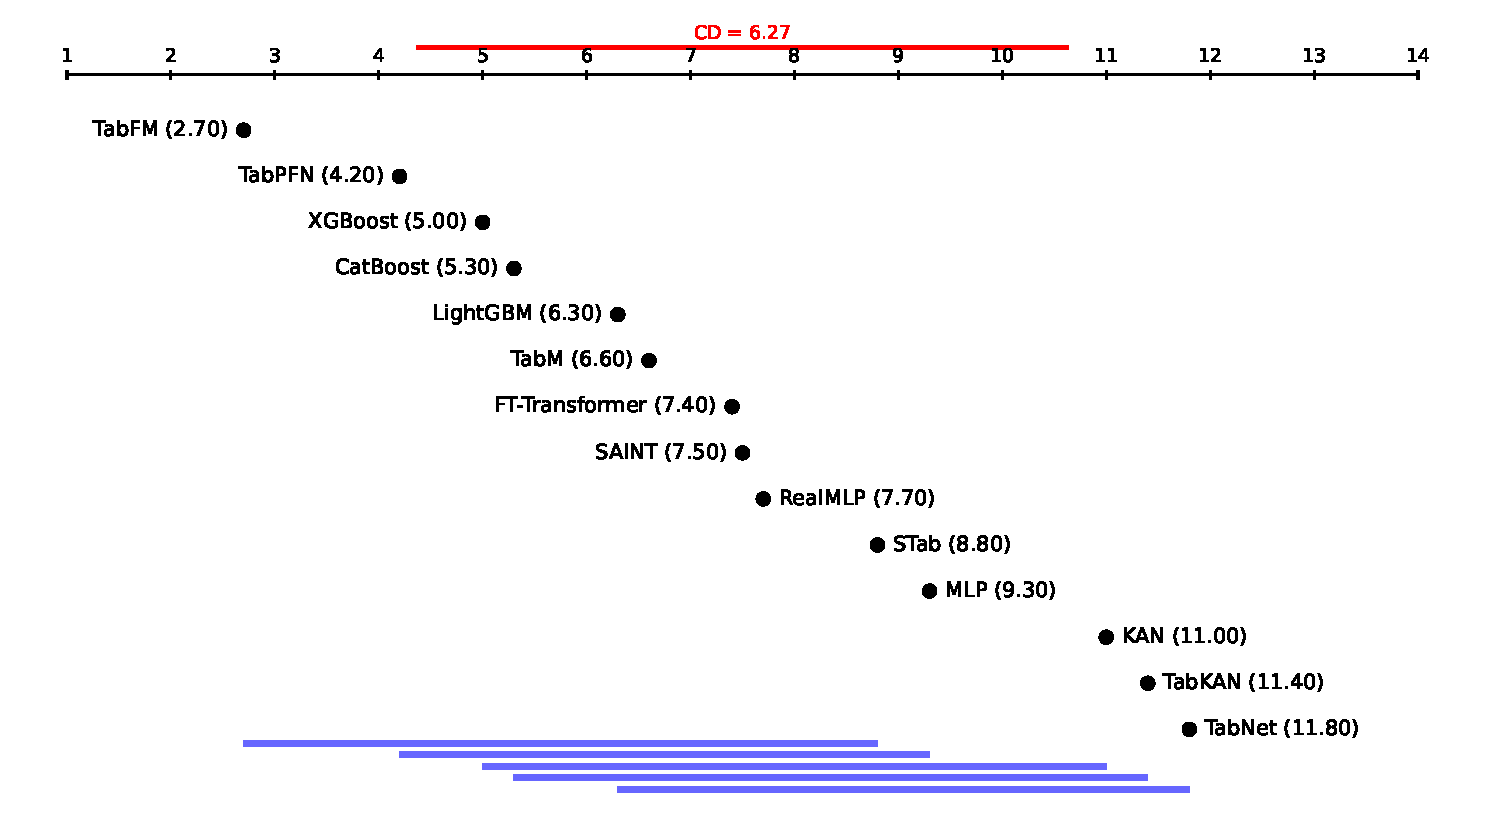
\includegraphics[width=0.9\linewidth]{images/cd_diagram_binary.pdf}
\caption[Diagrama de distância crítica (Nemenyi) --- classificação
binária]{\textbf{O post-hoc não separa o pelotão superior: as barras
horizontais conectam grupos estatisticamente inseparáveis, e elas são
largas.} Diagrama de distância crítica (Nemenyi) para a classificação
binária, todos os 14 modelos ($N{=}10$ conjuntos, CD $= 6{,}27$). O eixo
é o rank médio (menor é melhor); modelos a uma distância menor que a
barra CD não são estatisticamente separáveis, e cada barra horizontal na
parte inferior conecta um grupo inseparável --- a largura dessas barras é
a forma visual da cautela sobre o CD largo discutida na
Seção~\ref{sec:cap5-ato4}. As estatísticas do Ato~I no texto restringem-se
ao núcleo de 11 modelos. Rótulos internos da figura em inglês e decimais com ponto (figura canônica do \emph{benchmark}); eixos e leitura descritos nesta legenda. Fonte:
\texttt{latex/ai1/figures/cd\_diagram\_binary.pdf}.}
\label{fig:cap5-cd}
\end{figure}

A interpretação exige a ressalva imediata: um post-hoc que não separa
não é, por si só, evidência de equivalência --- com $k$ grande e $N$
pequeno, a distância crítica é larga por construção, e ``não separável''
pode significar apenas ``sem poder para separar''. É exatamente por isso
que o protocolo pré-registrou instrumentos mais finos, apresentados no
Capítulo~\ref{chap:fundamentacao} e aplicados a seguir.

\paragraph{A leitura bayesiana: equivalência prática, não ausência de
poder.}
O teste bayesiano \emph{signed-rank} com região de equivalência prática
(ROPE) \citep{benavoli2017} responde à pergunta que o frequentista não
alcança: qual a probabilidade de a diferença entre dois modelos ser
\emph{praticamente irrelevante}? Com ROPE de $\pm$0,01 de AUC, o teste
declara \textbf{8 dos 10} modelos não-líderes praticamente equivalentes
ao líder de rank do núcleo (TabPFN). A análise de sensibilidade do
limiar --- pré-registrada precisamente para evitar que a conclusão
dependa de uma escolha arbitrária --- mostra a progressão
$0{,}005/0{,}01/0{,}02 \to 2/8/10$ equivalentes: a conclusão de empate
vale na margem de um ponto percentual de AUC. Lendo massa posterior
acima de 0,5 como ``mais provavelmente equivalente que não'', o XGBoost
($P(\mathrm{equiv}) = 0{,}65$) supera essa barra mesmo no limiar
estrito de 0,005, com o CatBoost no limite (0,54). O empate do topo,
portanto, não é um artefato de baixo poder: é equivalência prática
positivamente aferida.

\achado{5.1}{No núcleo de 11 modelos, o topo da classificação binária é um
empate estatístico: 8 dos 10 modelos não-líderes são praticamente
equivalentes ao líder sob ROPE de $\pm$0,01 de AUC, e a conclusão
sobrevive à variação do limiar.}
O omnibus rejeita a igualdade global, mas o post-hoc não separa o
pelotão superior e o instrumento bayesiano declara equivalência prática
--- a máxima ``boosting sempre vence'' não encontra, nessa geração,
margem de acurácia que a sustente.

\paragraph{O escopo do empate: onde há poder para afirmá-lo.}
Uma delimitação honesta antes de prosseguir: o empate é estabelecido na
classificação binária, a única tarefa com $N$ suficiente ($N{=}10$) para
que os instrumentos operem com poder útil. Na regressão, $N{=}5$ impõe
um piso combinatório ao p-valor do teste de Wilcoxon pareado (0,0625 ---
nenhuma comparação pode cruzar o limiar convencional de 5\% ali, por
aritmética, não por ausência de efeito); na multiclasse, $N{=}3$ reduz
qualquer análise ao plano descritivo. Essas limitações são declaradas em
cada seção em que se tornam vinculantes, e nenhum achado numerado deste
capítulo depende de significância em tarefa sem poder para aferi-la.

\paragraph{A anatomia do empate: a família é uma abstração fraca.}
Se o topo empata, resta perguntar o que, afinal, explica a variação de
desempenho que existe. A decomposição de variância de ranks por família
responde: $\eta^2 = 0{,}20$ --- apenas 20\% da variância de rank é
explicada pelo pertencimento à família (GBDT, DL, \emph{foundation model}), e
\textbf{80\% é intrafamília}. ``GBDT vs.\ DL'', o eixo em torno do qual a
literatura organizou a década, é uma abstração fraca para esses dados: o
modelo específico importa mais que a família a que pertence. Uma
ressalva de leitura acompanha o número: com as famílias desbalanceadas do
núcleo (3 GBDTs, 7 DL, 1 \emph{foundation model}), essa partição é mecanicamente
conservadora --- ainda assim, a ordem de grandeza da razão
intra/entre-famílias sustenta a conclusão qualitativa.

\achado{5.2}{Oitenta por cento da variância de rank é intrafamília
($\eta^2 = 0{,}20$): escolher bem o modelo dentro da família importa mais
do que escolher a família.}
Esse achado reorienta a pergunta prática de ``qual família?'' para ``qual
modelo, sob quais restrições?'' --- a semente do arcabouço do
Capítulo~\ref{chap:framework}.

\paragraph{O que o agregado esconde: a visão por conjunto.}
O diagrama de distância crítica e o $\eta^2$ operam sobre ranks
agregados; nenhum dos dois mostra as magnitudes absolutas nem onde,
conjunto a conjunto, as diferenças moram. A
Figura~\ref{fig:cap5-heatmap} complementa essa lacuna com o mapa de calor
da classificação.

\begin{figure}[htbp]
\centering
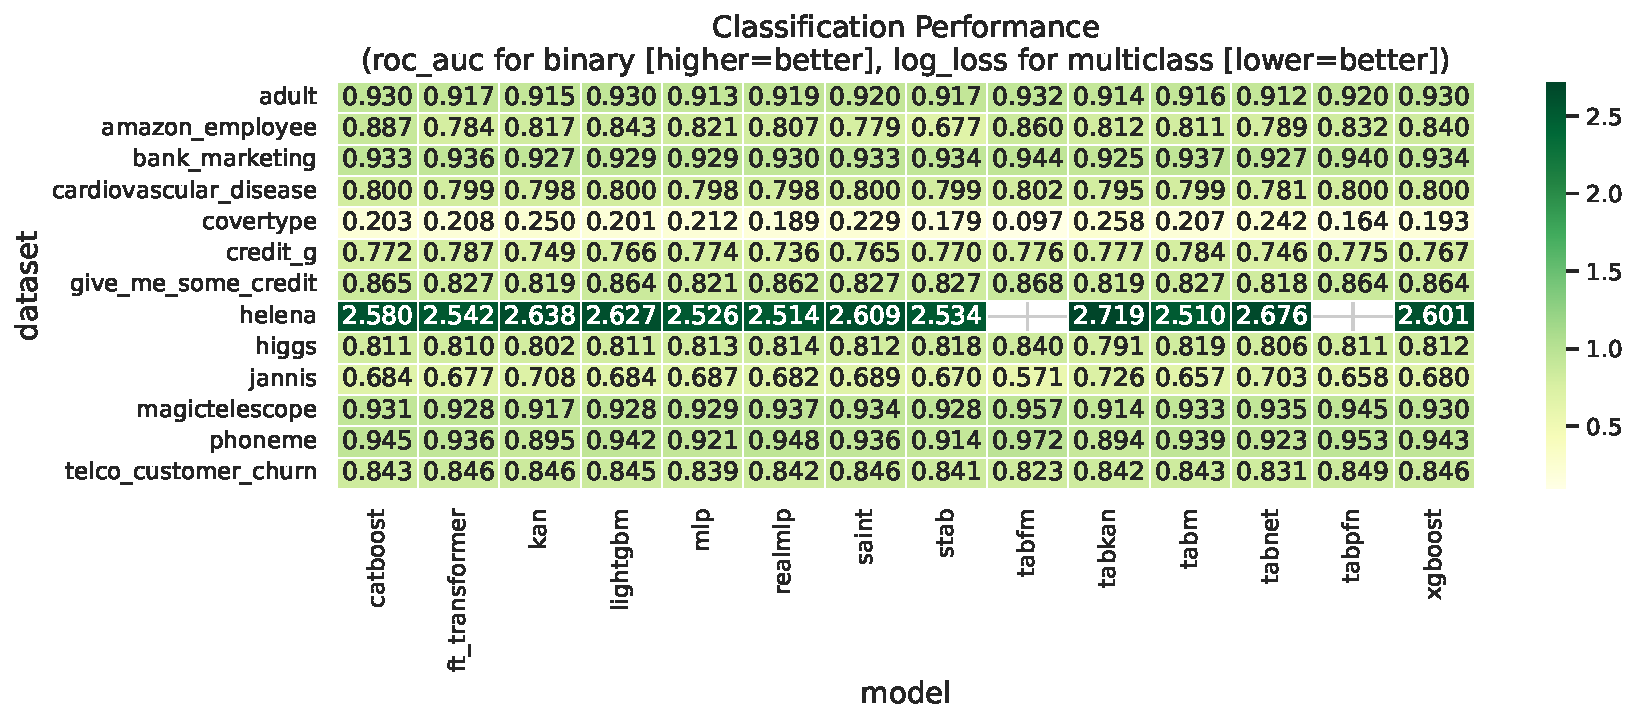
\includegraphics[width=\linewidth]{images/heatmap_classification.pdf}
\caption[Mapa de calor da classificação: métrica por modelo e
conjunto]{\textbf{As margens absolutas no topo são pequenas --- em vários
conjuntos binários, a diferença entre o melhor e a mediana dos modelos
está na segunda casa decimal de AUC.} Métrica primária por modelo
(colunas) e conjunto (linhas): ROC-AUC nas binárias (maior é melhor) e
log-loss nas multiclasse (menor é melhor) --- as duas métricas convivem
na mesma grade, de modo que a comparação válida é dentro de cada linha,
nunca entre linhas. As células vazias na linha \texttt{helena} são as
duas exclusões estruturais (TabPFN e TabFM, 100 classes acima do limite
arquitetural). Rótulos internos da figura em inglês e decimais com ponto (figura canônica do \emph{benchmark}); eixos e leitura descritos nesta legenda. Fonte:
\texttt{results/figures/heatmap\_classification.pdf}.}
\label{fig:cap5-heatmap}
\end{figure}

A leitura por conjunto confirma a do agregado --- margens pequenas no
topo das binárias --- e adiciona o que o agregado não mostra: as duas
células estruturalmente vazias ficam visíveis, e os poucos conjuntos em
que um modelo abre vantagem nítida (como o CatBoost em
\texttt{amazon\_employee}, de alta cardinalidade categórica) antecipam as
reversões condicionais do Ato~III. A ressalva permanece: valores de
\emph{hold-out} em uma única partição fixa não carregam, sozinhos, significância
--- eles ilustram; a inferência vem dos testes pareados sobre os folds.

\paragraph{O único sinal robusto do desempenho bruto está no fundo.}
Enquanto o topo empata, o fundo não: o TabNet \citep{arik2021} é
consistentemente o pior modelo da geração do núcleo, com ranks médios de
11,8 (binária), 11,7 (multiclasse) e 11,4 (regressão) na grade completa.
É o único veredito de desempenho bruto que o benchmark autoriza sem
qualificação dentro do núcleo --- e um lembrete de que arquiteturas
celebradas na literatura podem não sobreviver a um protocolo uniforme
com orçamento de ajuste equalizado.

\section{Ato II --- os eixos de custo}
\label{sec:cap5-ato2}

Se a acurácia empata, a decisão entre os modelos do topo precisa de
outros eixos --- e é neles que os modelos diferem radicalmente. Esta
seção percorre os três eixos de custo medidos pelo protocolo (tempo de
treino, custo de ajuste de hiperparâmetros e latência de inferência) e os
cruza com o desempenho na fronteira de Pareto.

\paragraph{Treino: duas ordens e meia de magnitude.}
O tempo de treino mediano varia cerca de $300\times$ dentro da grade:
LightGBM e XGBoost ajustam o modelo final em ${\sim}0{,}7$~s, enquanto
SAINT e STab consomem ${\sim}200$~s por ajuste --- e a diferença se
multiplica pelo número de tentativas de ajuste de hiperparâmetros e de
folds da validação cruzada aninhada. Os \emph{foundation models} invertem o
eixo: por serem \emph{zero-shot}, o ``treino'' do TabFM custa 0,18~s e o
do TabPFN 1,35~s, com custo de ajuste \textbf{zero} --- não há busca de
hiperparâmetros a pagar. Essa inversão, cujo outro lado aparece já no
próximo parágrafo, é o fio que costura o capítulo.

\paragraph{Ajuste de hiperparâmetros: o custo escondido.}
O segundo eixo é o custo total do ajuste de hiperparâmetros, que o tempo
de treino de um único ajuste subestima. Nas medianas entre conjuntos, os
GBDTs pagam de 106~s (LightGBM) a 648~s (CatBoost) pelo ciclo completo de
busca; o DL tipo-MLP paga de 1.150~s (MLP) a 3.515~s (TabM); e a atenção
pesada chega a 12.245~s (SAINT) e 14.956~s (STab) --- duas ordens de
magnitude acima dos GBDTs mais baratos, para, como visto no Ato~I, não
sair do empate. Os \emph{foundation models} pagam zero. Esse eixo raramente
aparece nos benchmarks da literatura, mas é o que o praticante paga a
cada reajuste do modelo em produção.

\paragraph{Inferência: cinco ordens de magnitude.}
A latência de inferência é o eixo mais dramático do benchmark. A
Figura~\ref{fig:cap5-latencia} apresenta a medição completa, feita sob
protocolo idêntico para os 14 modelos: \us{} por linha, mediana de 5
passadas sobre o \emph{hold-out} completo do \texttt{adult}, cada modelo em seu
dispositivo natural (GBDTs em CPU; modelos profundos e \emph{foundation models}
em GPU).

\begin{figure}[htbp]
\centering
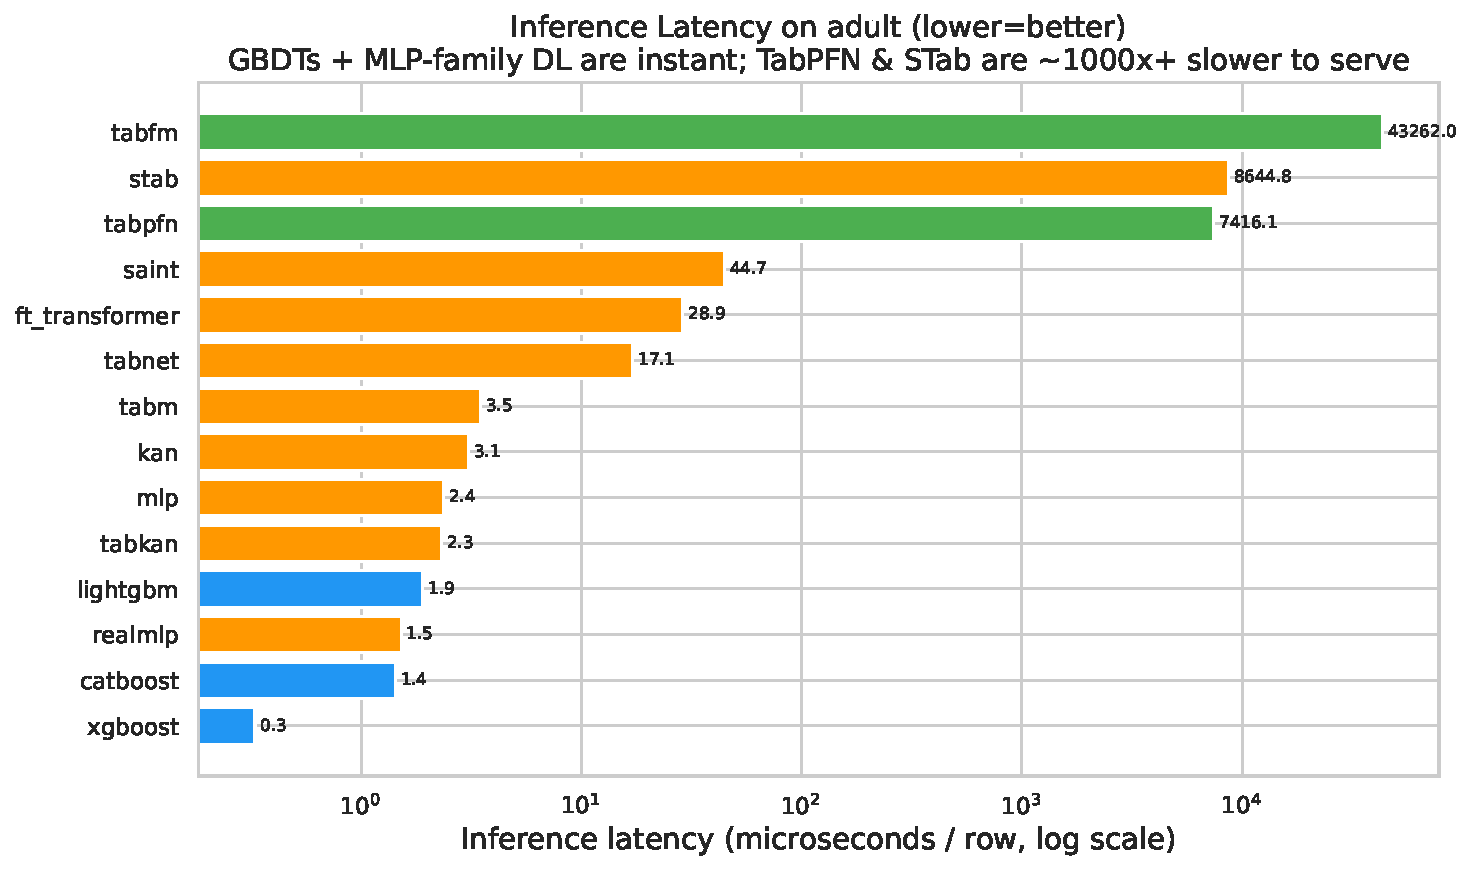
\includegraphics[width=0.95\linewidth]{images/inference_time.pdf}
\caption[Latência de inferência no \texttt{adult} (\us/linha, escala
logarítmica)]{\textbf{A latência de inferência atravessa cinco ordens de
magnitude: GBDTs e DL tipo-MLP servem em microssegundos; atenção custa
dezenas de \us; os paradigmas de inferência pesada custam milhares.}
Latência em \us{} por linha no \emph{hold-out} do \texttt{adult} (mediana de 5
passadas, escala logarítmica, menor é melhor), com cores por família.
Cada modelo roda em seu dispositivo natural (GBDTs em CPU; profundos e
\emph{foundation models} em GPU), de modo que as razões descrevem o regime de
serving em lote amortizado em uma máquina declarada --- não a latência
online de linha única, cujas diferenças são menores. Rótulos internos da figura em inglês e decimais com ponto (figura canônica do \emph{benchmark}); eixos e leitura descritos nesta legenda. Fonte:
\texttt{results/figures/inference\_time.pdf} (dados em
\texttt{results/latency/latency\_adult.csv}).}
\label{fig:cap5-latencia}
\end{figure}

A estrutura da figura organiza-se em quatro camadas. Na base, o XGBoost
serve a 0,33~\us/linha. O \emph{tier} rápido reúne os três GBDTs, os
modelos profundos tipo-MLP e as duas KANs (CatBoost 1,4; RealMLP 1,5;
LightGBM 1,9; TabKAN 2,3; MLP 2,4; KAN 3,1; TabM 3,5~\us/linha) --- um
resultado em si: aprendizado profundo \emph{não} é sinônimo de serviço
caro; a arquitetura é que decide. A atenção custa dezenas de
microssegundos (TabNet 17; FT-Transformer 29; SAINT 45). E o extremo
pertence aos paradigmas de inferência estruturalmente pesada: TabPFN
7.416, STab 8.645 e TabFM 43.262~\us/linha --- o custo do STab vem da
inferência bayesiana que calcula a média de 64 passadas estocásticas; o
dos \emph{foundation models}, de carregar o conjunto de treino como contexto a
cada predição. A ressalva de regime, dita na legenda, merece repetição
no corpo: essas razões descrevem o serviço em lote amortizado no
hardware declarado no Capítulo~\ref{chap:metodologia}; o serviço online
de linha única estreita as diferenças --- mas não as ordens de
magnitude.

\paragraph{O cruzamento: a fronteira de Pareto.}
Nenhum dos eixos isolados decide; o instrumento de decisão é o
cruzamento desempenho $\times$ custo. Sobre rank médio $\times$ custo
--- sendo o rank o instrumento primário de comparação do estudo --- o
núcleo de 11 modelos resolve-se em uma fronteira de Pareto de
\{TabPFN, XGBoost, LightGBM\} no eixo de custo de treino, que se estreita
para \{XGBoost, TabPFN\} no eixo de latência (sobre AUC média em vez de
rank, o CatBoost também entra na fronteira --- e, no eixo de latência, o
TabPFN sai dela); \textbf{todo o
aprendizado profundo clássico é dominado} em ambos os cruzamentos. A
Figura~\ref{fig:cap5-pareto} apresenta o retrato completo, já com os 14
modelos.

\begin{figure}[htbp]
\centering
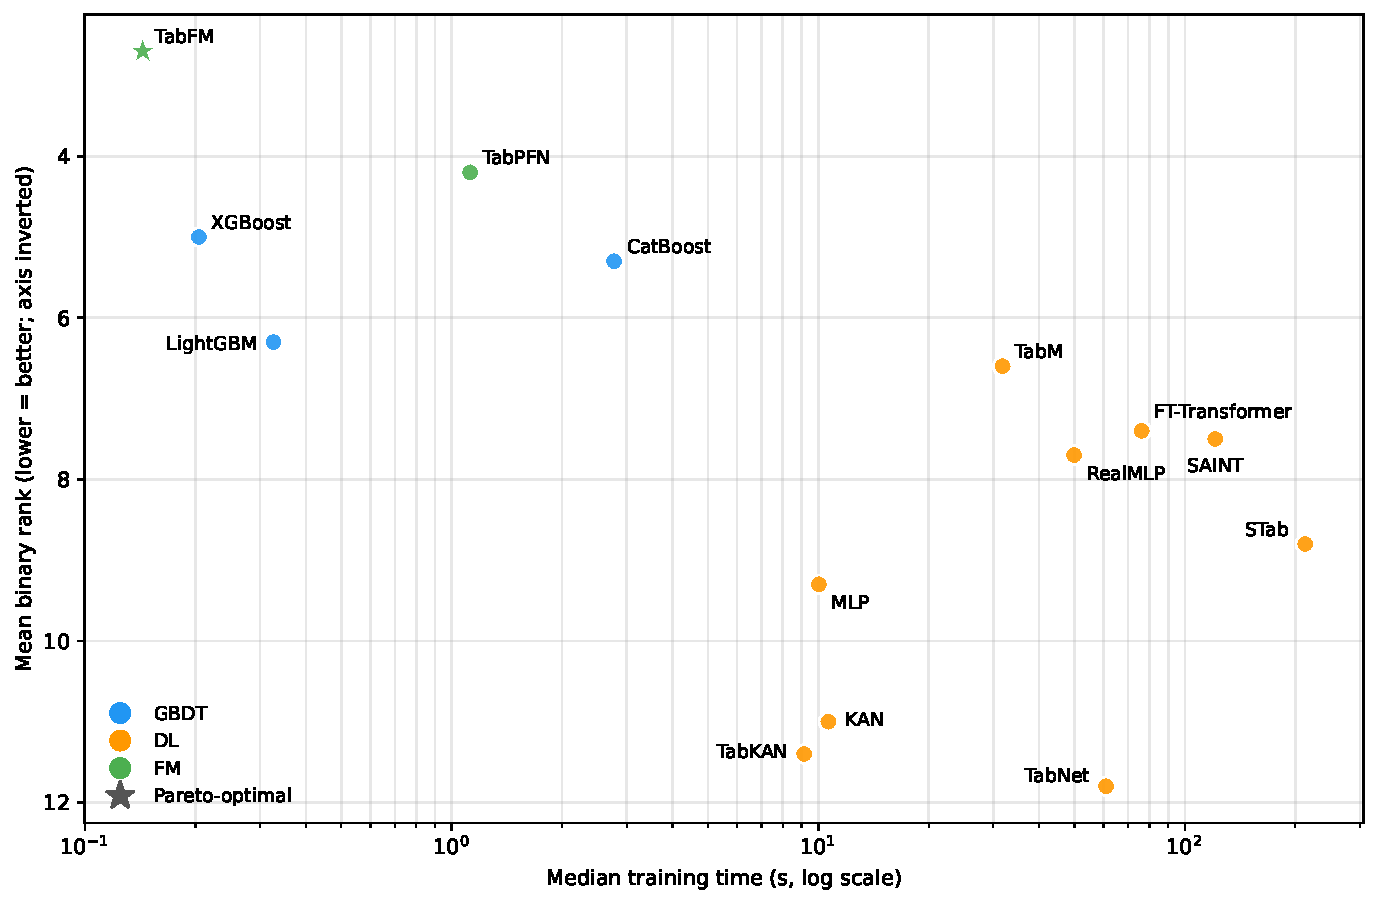
\includegraphics[width=0.92\linewidth]{images/pareto_binary.pdf}
\caption[Fronteira de Pareto: rank binário médio vs.\ tempo de
treino]{\textbf{Na grade completa, o TabFM toma a fronteira
treino-desempenho sozinho: é simultaneamente o ajuste mais barato e o
melhor rank.} Rank binário médio $\times$ tempo mediano de treino sobre
os conjuntos binários (escala logarítmica; o eixo de rank é invertido, de
modo que acima-à-esquerda é melhor), todos os 14 modelos. O ponto
estrelado é Pareto-ótimo sobre a grade completa (TabFM); a fronteira
\{TabPFN, XGBoost, LightGBM\} citada no texto é a restrição ao núcleo de
11 modelos. As comparações sobre o eixo de latência de inferência são
reportadas no texto. Rótulos internos da figura em inglês e decimais com ponto (figura canônica do \emph{benchmark}); eixos e leitura descritos nesta legenda. Fonte:
\texttt{latex/ai1/figures/pareto\_binary.pdf}.}
\label{fig:cap5-pareto}
\end{figure}

A figura mostra o que a latência isolada não mostra: no plano
treino $\times$ rank, os \emph{foundation models} ocupam o canto ótimo --- e é
só ao trocar o eixo de custo para a latência de serviço que a imagem se
inverte. Essa dupla leitura é o \textbf{achado-âncora do programa}: o
paradigma de \emph{in-context learning} compra treino de segundos e
ajuste zero ao preço de serviço proibitivo. É ela que motiva tanto o
eixo de restrições do arcabouço de decisão
(Capítulo~\ref{chap:framework}) quanto a pergunta da destilação
(Capítulo~\ref{chap:destilacao}): quanto desse preço é removível?

\achado{5.3}{Modelos praticamente equivalentes em acurácia diferem em
${\sim}300\times$ no tempo de treino e em cinco ordens de magnitude na
latência de inferência; no núcleo de 11, a fronteira de Pareto
rank~$\times$~custo é \{TabPFN, XGBoost, LightGBM\} no eixo de treino ---
e todo o aprendizado profundo clássico é dominado.}
Quando o desempenho empata, o custo decide --- e o custo não empata.

\section{Ato III --- reversões condicionais e o eixo do tamanho}
\label{sec:cap5-ato3}

O empate do Ato~I é um retrato agregado; ele não implica que todos os
problemas sejam iguais. Este ato condiciona os resultados à estrutura da
tarefa e ao tamanho amostral, e encontra reversões reais --- a matéria-prima
das perguntas de restrição do Capítulo~\ref{chap:framework}.

\paragraph{Multiclasse: o DL recente assume o topo clássico.}
Na classificação multiclasse, os modelos profundos da geração mais
recente (STab e TabM, ambos com rank médio 3,67 na grade completa) tomam
o topo clássico dos GBDTs (XGBoost, o melhor deles, fica em 6,0). A
ressalva de poder é vinculante e repetida sempre que a multiclasse
aparece: com $N{=}3$ conjuntos, a análise é \textbf{descritiva} --- não
há teste com poder útil sobre três pontos --- e por isso nenhum achado
numerado se apoia exclusivamente nela.

\paragraph{Desbalanceamento severo: vantagem relativa dos GBDTs.}
A segunda reversão aparece ao estratificar os conjuntos de classificação
pela razão de desbalanceamento. A Figura~\ref{fig:cap5-imbalance}
apresenta os ranks médios agregados por família em três faixas de
severidade.

\begin{figure}[htbp]
\centering
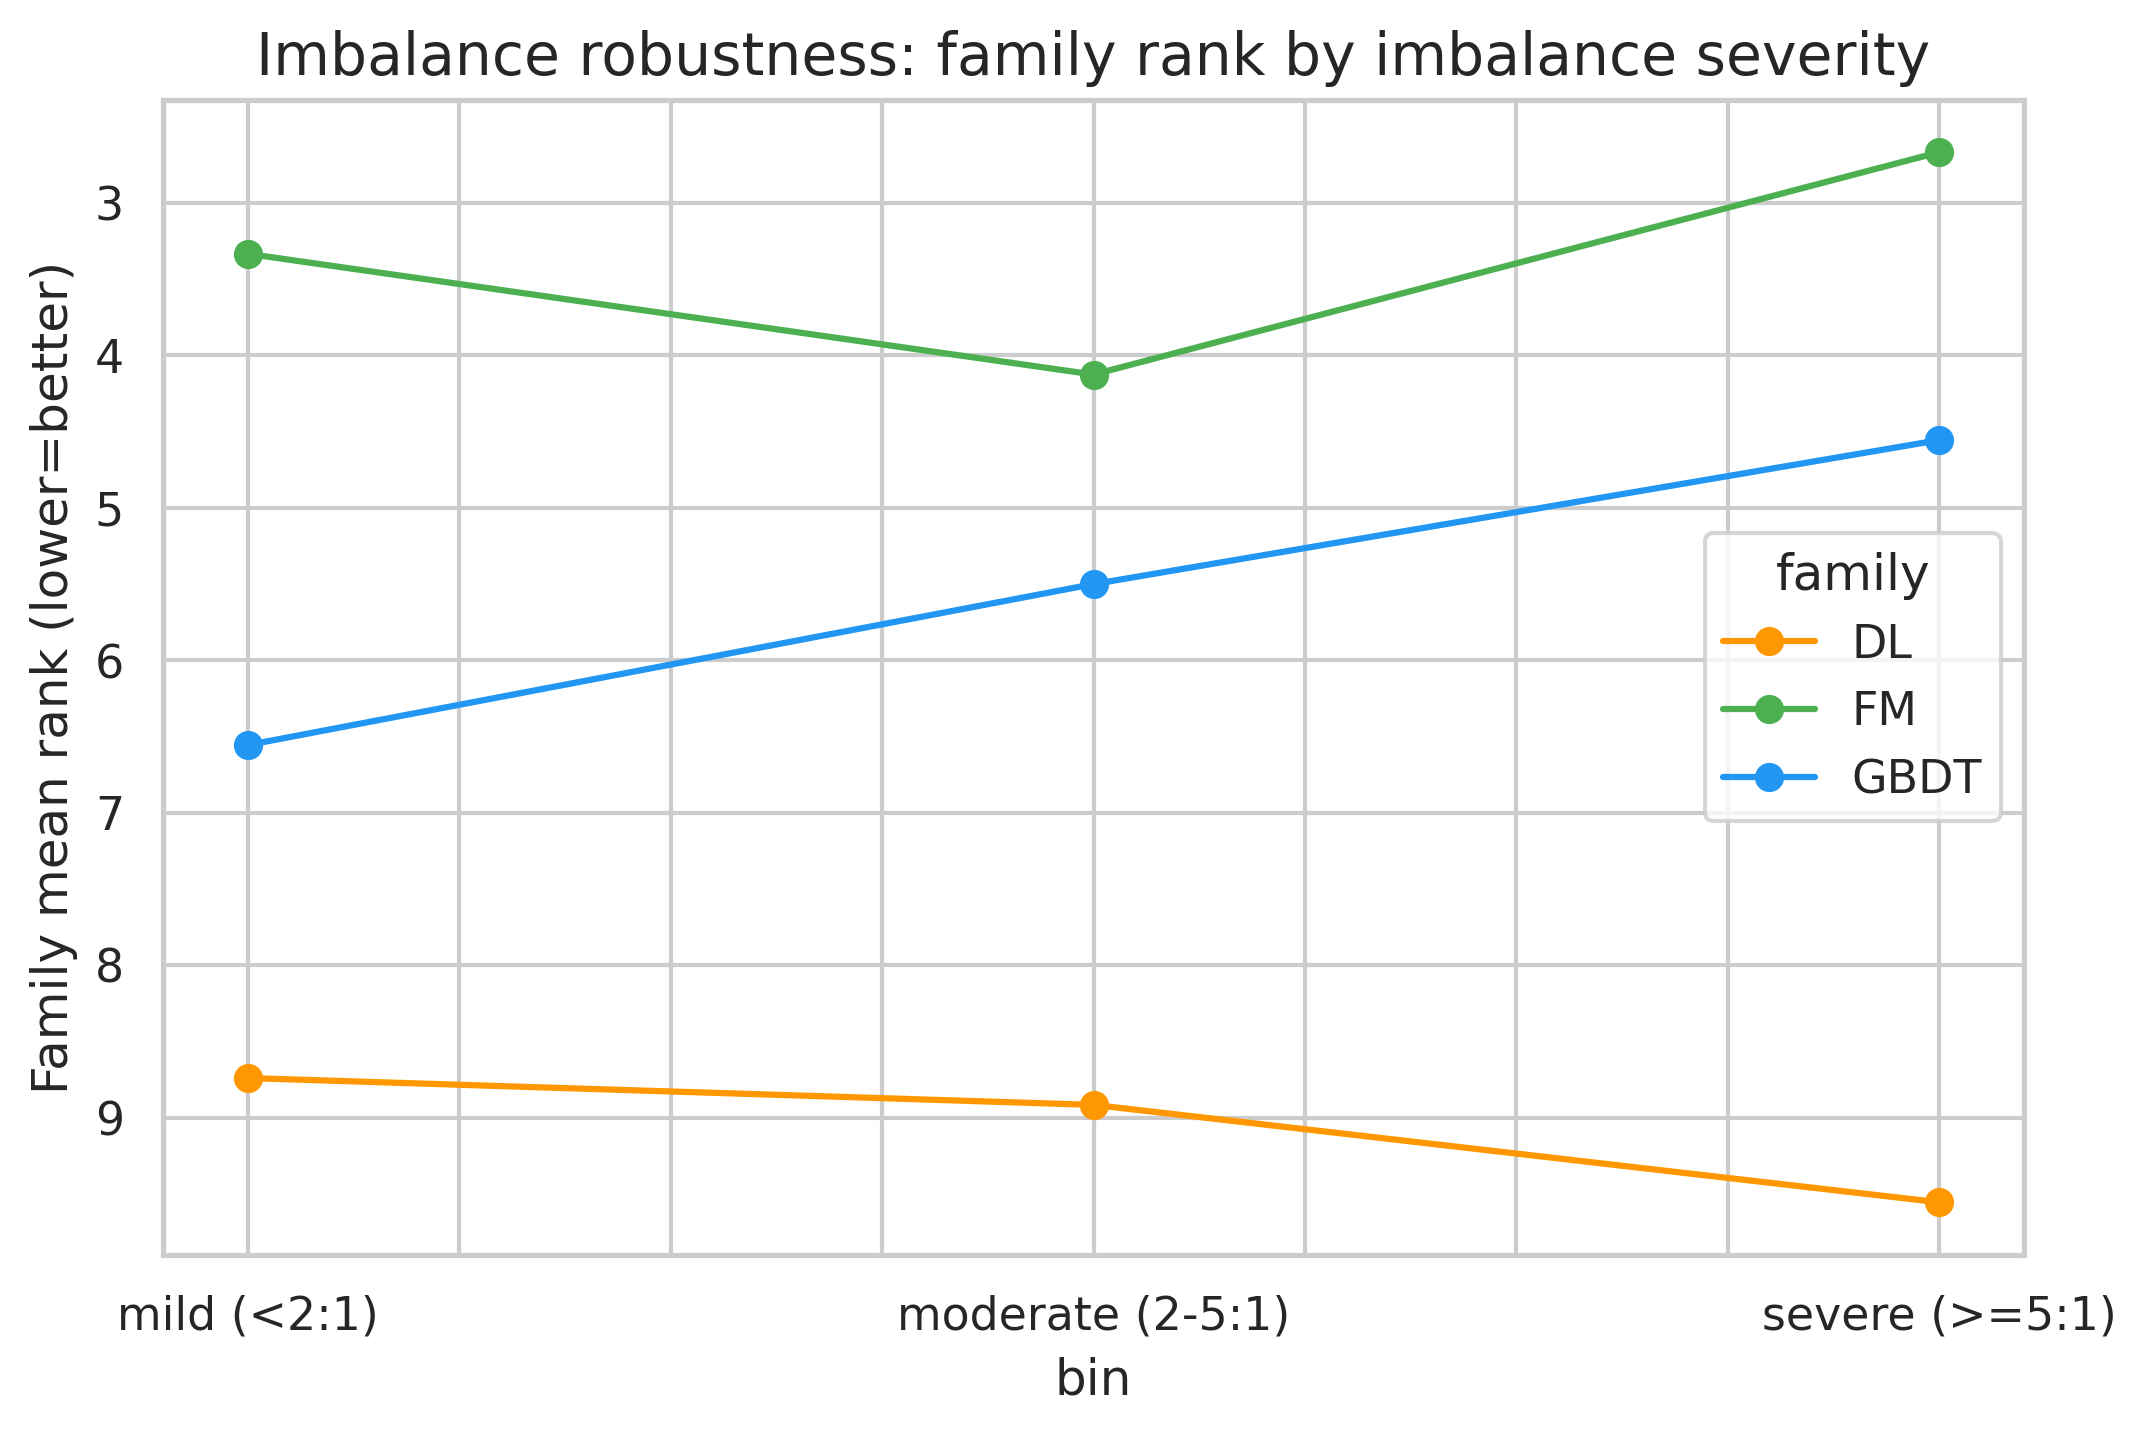
\includegraphics[width=0.85\linewidth]{images/imbalance_robustness.png}
\caption[Robustez ao desbalanceamento: rank por família e faixa de
severidade]{\textbf{Conforme o desbalanceamento se agrava, os GBDTs
melhoram seu rank relativo e o aprendizado profundo clássico piora; os
\emph{foundation models} permanecem à frente em todas as faixas.} Rank médio
agregado por família (menor é melhor; eixo invertido) nos conjuntos de
classificação, estratificados pela razão de desbalanceamento
majoritária/minoritária: leve ($<$2:1), moderada (2--5:1) e severa
($\geq$5:1). Ressalva: com poucos conjuntos por faixa, a figura é
descritiva --- ela indica direção de tendência, não significância.
Rótulos internos da figura em inglês e decimais com ponto (figura canônica do \emph{benchmark}); eixos e leitura descritos nesta legenda. O subtítulo embutido na figura (``$\sim$1000x+ slower to serve'') é um arredondamento editorial conservador da geração dela; os fatores medidos são os do texto (TabPFN 22.473$\times$, TabFM 131.097$\times$). Fonte: \texttt{results/figures/imbalance\_robustness.png}
(\texttt{notebooks/07\_segmented\_robustness.ipynb}).}
\label{fig:cap5-imbalance}
\end{figure}

A tendência é monotônica e na direção que a intuição de praticantes
sugere --- árvores lidam melhor com classes raras do que redes treinadas
por gradiente sobre perda média --- mas a ressalva da legenda é parte do
resultado: com poucos conjuntos por faixa, trata-se de direção
descritiva, não de teste. Duas observações completam o quadro
condicional: no extremo de cardinalidade categórica, a codificação
one-hot penaliza os modelos de atenção (o caso
\texttt{amazon\_employee} visível na Figura~\ref{fig:cap5-heatmap}); e o
TabPFN combina, dentro do núcleo, o melhor rank médio com o melhor
pior-caso --- é o modelo que mais raramente falha de forma catastrófica,
um atributo de robustez que rank médio sozinho não captura.

\paragraph{O eixo do tamanho: curvas de aprendizado.}
Nenhuma das análises anteriores responde à pergunta mais frequente do
praticante: ``com \emph{meu} volume de dados, quem vence?''. As curvas
de aprendizado --- 6 modelos $\times$ 5 conjuntos $\times$ 3 sementes,
varrendo de 500 amostras ao \emph{pool} completo --- dão forma a esse eixo. A
Figura~\ref{fig:cap5-curvas} apresenta a varredura completa.

\begin{figure}[htbp]
\centering
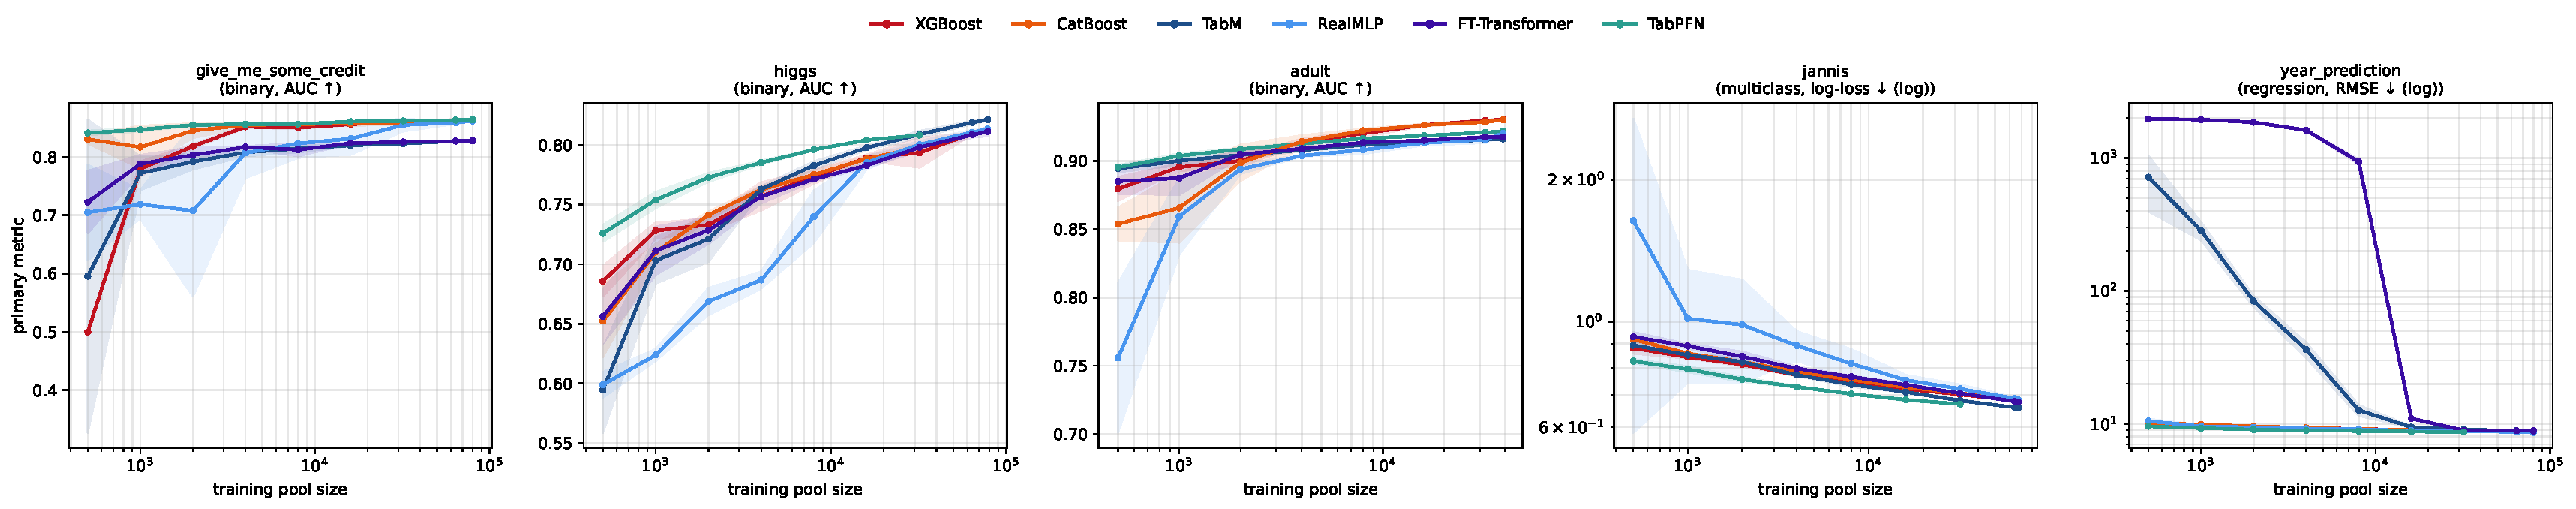
\includegraphics[width=\linewidth]{images/learning_curves.pdf}
\caption[Curvas de aprendizado: 6 modelos, 5 conjuntos, 500 amostras ao
pool completo]{\textbf{O cruzamento de liderança GBDT$\leftrightarrow$DL
é real, mas específico por conjunto --- e o TabPFN lidera o regime de
poucos dados em todos os cinco painéis.} Curvas de aprendizado (6
modelos $\times$ 5 conjuntos $\times$ 3 sementes, de 500 amostras ao \emph{pool}
completo). Cada painel nomeia sua métrica e direção ($\uparrow$ maior é
melhor; $\downarrow$ menor, escala logarítmica); as bandas são $\pm$1
desvio-padrão sobre as sementes. Um cruzamento é o ponto em que a curva
de uma família cruza permanentemente a da outra. Rótulos internos da figura em inglês e decimais com ponto (figura canônica do \emph{benchmark}); eixos e leitura descritos nesta legenda. Fonte:
\texttt{latex/ai1/figures/learning\_curves.pdf}
(\texttt{notebooks/10\_learning\_curves.ipynb}).}
\label{fig:cap5-curvas}
\end{figure}

Três leituras saem da figura. Primeira: o cruzamento de liderança entre
GBDTs e DL existe, mas é específico por conjunto --- em 3 dos 5
conjuntos varridos (\texttt{higgs}, \texttt{jannis} e
\texttt{year\_prediction}), o DL ultrapassa os GBDTs e não devolve a
liderança; no \texttt{adult}, o GBDT a retoma em $n \approx 4.000$; e em
\texttt{give\_me\_some\_credit}, o GBDT lidera do início ao fim. Não há,
portanto, um ``$n$ crítico'' universal a recomendar: a resposta honesta
ao praticante é que o cruzamento depende do conjunto, não apenas do
tamanho. Segunda: o TabPFN
tem a melhor métrica média de regime nos cinco conjuntos varridos para
$n \leq 4.000$ (rank médio 1,0 nesse regime, contra 2,8 do XGBoost) ---
a quantificação do nicho de poucos dados do paradigma \emph{zero-shot}.
Terceira, a ressalva: a varredura cobre 6 dos 14 modelos e 5 dos 18
conjuntos; ela qualifica o eixo do tamanho, não o reordena.

\achado{5.4}{A melhor família depende da estrutura do problema --- o DL
recente toma o topo multiclasse (descritivo), os GBDTs ganham vantagem
relativa sob desbalanceamento severo, o one-hot penaliza a atenção no
extremo categórico --- e o cruzamento GBDT$\leftrightarrow$DL por
tamanho é real mas específico por conjunto, com o TabPFN dominando o
regime $n \leq 4.000$ em todos os conjuntos varridos.}
As reversões não restauram a máxima de uma família vencedora: elas
mostram que a resposta certa é condicional --- e condições verificáveis
a priori são exatamente o que um arcabouço de decisão pode codificar.

\section{Ato IV --- a quebra do empate: a geração 2026}
\label{sec:cap5-ato4}

\paragraph{A entrada do TabFM reorganiza a narrativa.}
A expansão para a grade completa de 14 modelos muda o retrato. O TabFM
--- \emph{foundation model} lançado em junho de 2026, avaliado aqui
\emph{zero-shot}, sem qualquer ajuste por conjunto --- lidera o rank
médio \textbf{nas três tarefas}: 2,7 na binária, 1,0 na multiclasse
(pontuação perfeita sobre seus dois conjuntos elegíveis;
\texttt{helena} é exclusão estrutural) e 1,2 na regressão. É o melhor
modelo absoluto em \textbf{13 dos 18 conjuntos}, participando de 17. A
Tabela~\ref{tab:cap5-ranks} resume os ranks por tarefa e a
Figura~\ref{fig:cap5-ranks} apresenta o retrato visual.

\begin{table}[htbp]
\centering
\caption[Rank médio por tarefa --- geração 2026 vs.\ referências]{Rank
médio por tarefa --- geração 2026 vs.\ referências ($k{=}14$ modelos;
binária $N{=}10$, multiclasse $N{=}3$, regressão $N{=}5$; menor é melhor,
\textbf{negrito} = melhor da coluna). Os ranks multiclasse de TabFM e
TabPFN são médias sobre os 2 conjuntos excluindo \texttt{helena}
(exclusão estrutural). A tabela mestra completa, com a métrica primária
de cada modelo em cada um dos 18 conjuntos, está no
Apêndice~\ref{app:tabelas}. Fonte:
\texttt{notebooks/TABELA\_RESULTADOS.md}.}
\label{tab:cap5-ranks}
\begin{tabular}{lccc}
\toprule
 & Binária & Multiclasse & Regressão \\
\midrule
\textbf{TabFM}      & \textbf{2,7} & \textbf{1,00} & \textbf{1,2} \\
TabPFN              & 4,2          & 2,50          & 3,0 \\
Melhor clássico     & XGBoost 5,0  & STab/TabM 3,67 & XGBoost 5,0 \\
KAN                 & 11,0         & 12,0          & 9,8 \\
TabKAN              & 11,4         & 13,3          & 11,8 \\
\bottomrule
\end{tabular}
\end{table}

\begin{figure}[htbp]
\centering
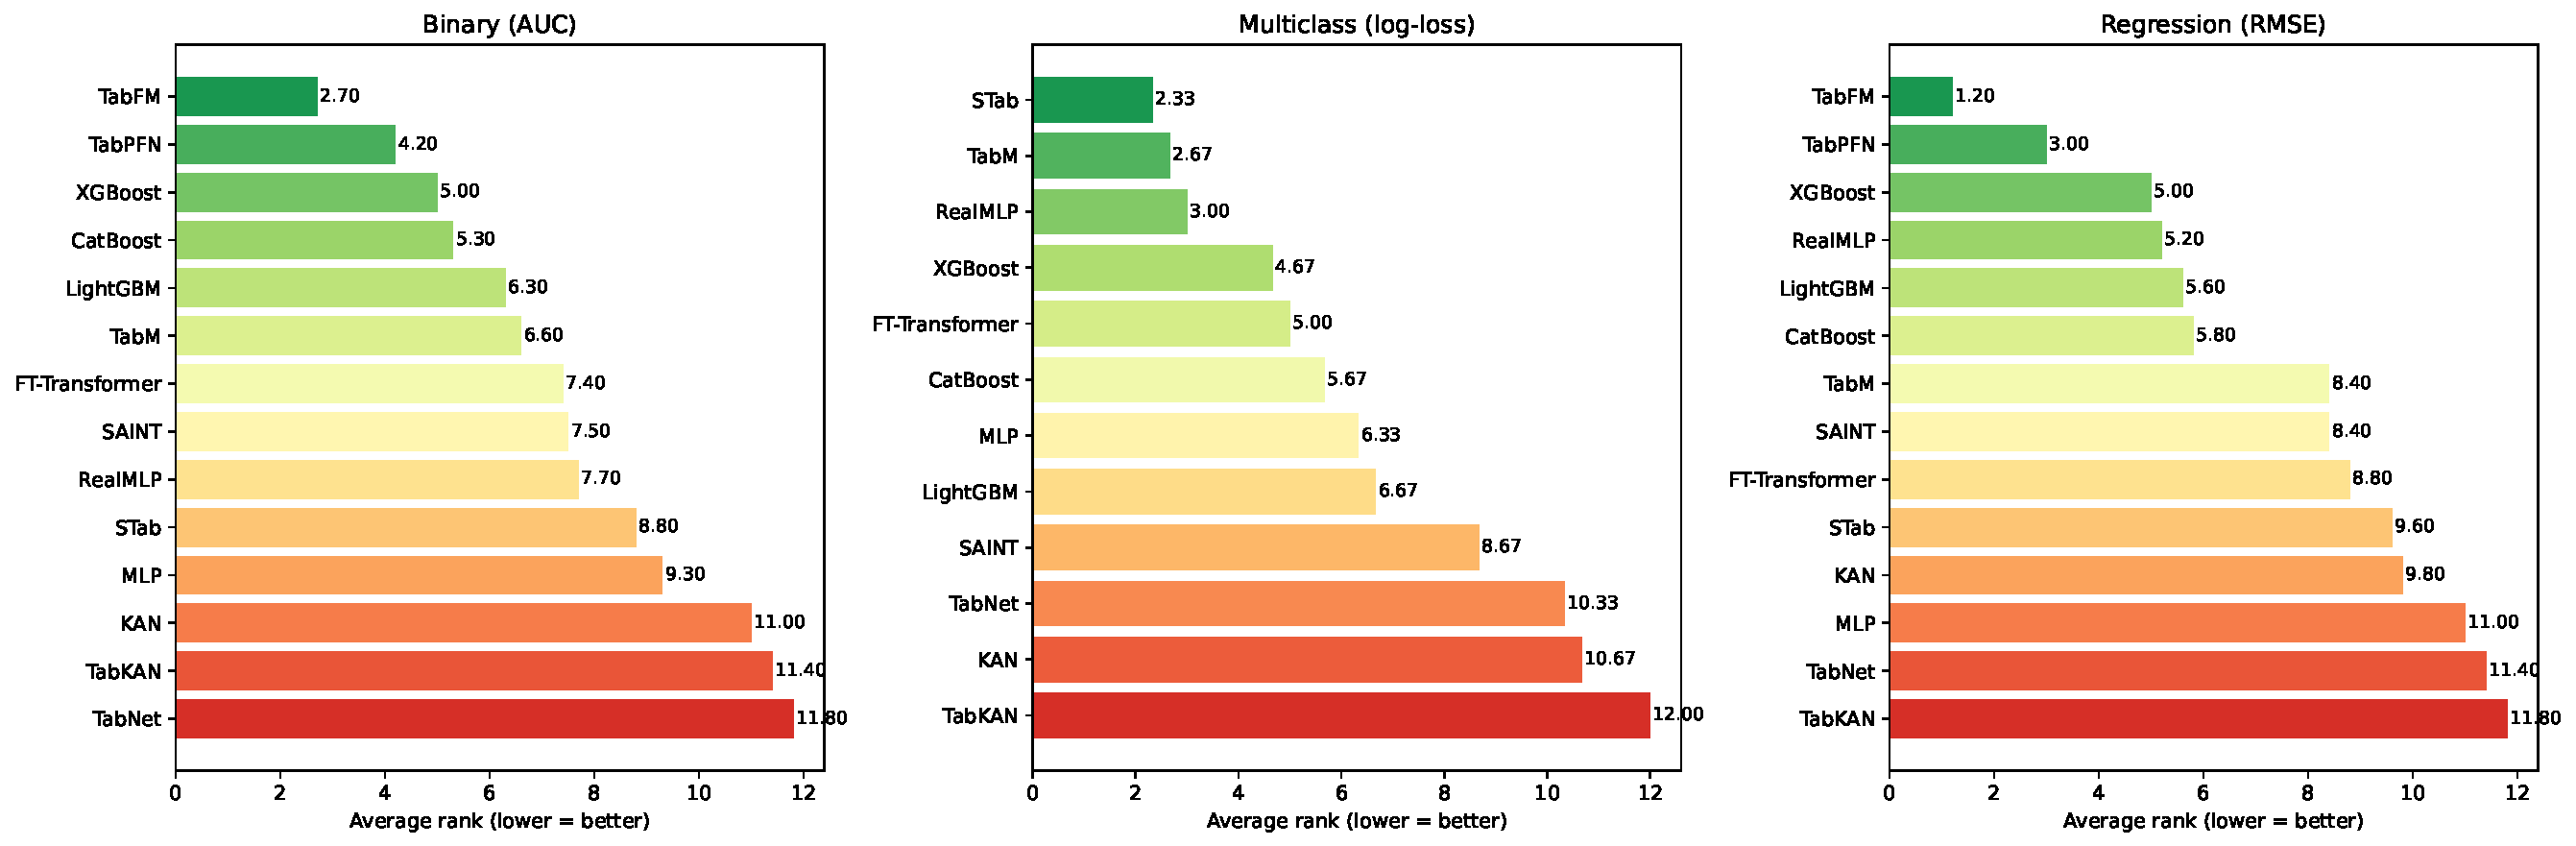
\includegraphics[width=0.92\linewidth]{images/average_ranks.pdf}
\caption[Ranks médios por tarefa, grade completa]{\textbf{A geração 2026
(TabFM) separa-se do pelotão nos painéis de binária e regressão; as KANs
ocupam o último terço em todos.} Ranks médios por tarefa. Os painéis de
binária e regressão cobrem os 14 modelos; o painel multiclasse mostra os
12 modelos avaliados nos três conjuntos multiclasse, rankeados dentro
desse subconjunto --- e por isso não é diretamente comparável aos ranks
de 14 modelos da Tabela~\ref{tab:cap5-ranks}, em que os foundation
models (excluídos no \texttt{helena}) são rankeados. Rótulos internos da figura em inglês e decimais com ponto (figura canônica do \emph{benchmark}); eixos e leitura descritos nesta legenda. Fonte:
\texttt{latex/ai1/figures/average\_ranks.pdf}.}
\label{fig:cap5-ranks}
\end{figure}

Dois detalhes concretos dão escala à liderança. Na multiclasse, onde a
margem é mais visível, o TabFM alcança log-loss de 0,0966 no
\texttt{covertype} e 0,5709 no \texttt{jannis}, contra 0,1644 e 0,6583
do segundo colocado (TabPFN) --- margens visivelmente maiores que as que
separam vizinhos de rank dentro do núcleo de 11 na mesma tabela
(Apêndice~\ref{app:tabelas}). E o TabPFN, por sua vez,
consolida-se como o vice consistente da grade (ranks médios
4,2/2,5/3,0 nas três tarefas): a geração 2026 não é um ponto fora da
curva, é uma família inteira --- os dois \emph{foundation models} ocupam os
dois primeiros postos em todas as tarefas.

A consequência interpretativa é a re-escopagem do Ato~I: o empate fica
corretamente lido como \emph{retrato da geração anterior}. Não foi o
aprendizado profundo ajustado que alcançou os GBDTs; foi o pré-treino que
atropelou ambos. E a cautela estatística permanece dita: com $k{=}14$ e
$N{=}10$, a distância crítica de Nemenyi é larga
(Figura~\ref{fig:cap5-cd}) --- a separação do TabFM apoia-se na
consistência entre conjuntos (13 vitórias em 18) e no instrumento
bayesiano, \textbf{não} no post-hoc frequentista. Duas condições de
contorno adicionais são declaradas: na regressão, $N{=}5$ põe o piso do
p-valor de Wilcoxon em 0,0625 (piso combinatório --- nenhum resultado
pode ser ``significativo a 5\%'' ali); e o TabFM é avaliado na versão
fixada v1.0.1 (julho de 2026), cujo relatório técnico oficial apareceu
apenas no fim de setembro de 2026 \citep{kong2026} e segue sem revisão
por pares --- os resultados são sobre essa versão, e isso fica
registrado.

\paragraph{O contrapeso: o líder de acurácia é o pior em latência.}
O contrapeso é frontal, e é o achado-âncora do programa: o líder de
acurácia é o pior modelo da grade em latência de serviço ---
43.262~\us/linha sob o protocolo padrão, $131.097\times$ o XGBoost, e
mais em contextos maiores, chegando a ${\sim}394$~ms/linha no maior
conjunto de regressão. A pergunta de decisão mudou de natureza: não é
mais ``qual família vence?'', e sim ``\emph{a latência do foundation
model cabe no caso de uso?}''.

\achado{5.5}{A geração 2026 quebra o empate: o TabFM lidera o rank médio
nas três tarefas e é o melhor modelo em 13 dos 18 conjuntos, \emph{zero-shot}
--- ao preço de quatro a cinco ordens de magnitude em latência de
serving (43.262 vs.\ 0,33~\us/linha).}
O empate não tornou o arcabouço multicritério obsoleto; a quebra o
tornou mais necessário --- e apontou seu único obstáculo.

\paragraph{O resultado negativo das redes de Kolmogorov--Arnold.}
No mesmo movimento da extensão, o benchmark produz o teste independente
da família Kolmogorov--Arnold --- e o resultado é o negativo de valor.
KAN (ranks 11,0/12,0/9,8 em binária/multiclasse/regressão) e TabKAN
(11,4/13,3/11,8) ocupam o último terço nas três tarefas, com o TabKAN
atrás até do TabNet em multiclasse e regressão. Surpreendente à luz das
alegações dos artigos originais \citep{kan2024,tabkan2025}, o resultado
pede explicação: sob protocolo uniforme com orçamento de ajuste
equalizado, as alegações não se sustentam, e a explicação mais provável
é que as comparações originais usaram \emph{baselines} subajustados ---
leitura consistente com a literatura cética anterior
\citep{poeta2024,kancritical2024}. Até onde alcança nossa verificação
datada de novidade, este é o primeiro teste da família contra a grade
completa GBDT/DL/foundation-model em um benchmark tabular multicritério;
as avaliações independentes anteriores
\citep{poeta2024,kancritical2024} comparam KANs apenas contra MLPs e não
medem eixos de custo. A contraparte de engenharia merece registro
simétrico: ambas habitam o \emph{tier} rápido de latência (2,3--3,1~\us/linha)
e custam VRAM desprezível --- \textbf{o problema é o desempenho, não o
custo}.

\achado{5.6}{Sob protocolo uniforme, KAN e TabKAN ficam no último terço
nas três tarefas --- as alegações dos artigos originais não se
sustentam no primeiro teste independente contra a grade completa, até
onde alcança nossa verificação datada --- embora ambas sejam baratas de
servir.}
O resultado negativo é reportado com o mesmo estatuto dos positivos,
conforme o contrato de conduta do estudo
(Capítulo~\ref{chap:metodologia}): um benchmark neutro existe
precisamente para que resultados assim venham a público.

\section{Síntese do capítulo}
\label{sec:cap5-sintese}

Três fatos encadeados emergem do benchmark. \textbf{(i)}~Na geração do
núcleo de 11 modelos, o desempenho bruto empata no topo --- empate
positivo, aferido por equivalência prática bayesiana e robusto à
variação do limiar --- e 80\% da variância de rank é intrafamília; a
decisão racional migra, portanto, para custo, latência, robustez e
estrutura da tarefa, exatamente os eixos em que os modelos diferem por
ordens de magnitude. \textbf{(ii)}~A geração 2026 quebra o empate em
acurácia: o TabFM lidera as três tarefas e vence em 13 de 18 conjuntos,
\emph{zero-shot} --- ao preço de quatro a cinco ordens de magnitude em latência
de serving, invertendo o eixo de custo (treino de segundos e ajuste
zero; serviço proibitivo). A quebra não aposenta a leitura
multicritério: ela a torna mais necessária, porque a escolha ótima
passa a depender de uma única restrição dominante. \textbf{(iii)}~Essa
restrição é atacável: a latência do \emph{foundation model} não é uma lei, é um
custo de arquitetura --- e custos de arquitetura podem ser transferidos
para modelos pequenos. As ressalvas do capítulo acompanham os fatos:
$N$ pequeno por tarefa (multiclasse descritiva; piso de p-valor na
regressão), distância crítica larga na grade completa, latências medidas
no regime de lote amortizado em dispositivo natural, e TabFM avaliado em
versão fixada anterior à revisão por pares de seu relatório técnico.

\begin{transicao}
O Capítulo~\ref{chap:framework} converte o fato (i) e as reversões do
Ato~III em um arcabouço de decisão por restrições --- e o valida por
\emph{leave-one-dataset-out}, testando tanto a alternativa de roteamento
por meta-características (resultado negativo) quanto a política fixa
``\emph{foundation model} primeiro, desviar por restrições'' (resultado
positivo). O obstáculo que resta a essa política --- as quatro a cinco
ordens de magnitude de latência do fato (ii) --- é o objeto do
Capítulo~\ref{chap:destilacao}: quanto dele a destilação remove, e sob
quais condições verificáveis.
\end{transicao}

%% ============================================================================
%% Capítulo 6 --- O Arcabouço de Decisão Validado
%%
%% Fontes (auditadas; nenhum número sem origem em artefato versionado):
%%   - dissertation/cap6-framework.md ............ prosa auditada; tabela de
%%     regret @11/@14 (idêntica à da AI-1)
%%   - latex/ai1/main.tex, seção "The Validated Decision Framework" ........
%%     formulação final auditada (taxa de acerto (\emph{hit-rate}) 0,11 vs 0,44 @11 e 0,72 vs 0,78
%%     @14; explicação do empate árvore/FM; rice1976; herre2026) --- prevalece
%%     sobre o rascunho em caso de divergência
%%   - docs/desenho-melhorias-finais.md, seção E2 .... pré-registro do regret
%%     multicritério ponderado (05/10/2026, antes da execução)
%%   - results/aggregated/lodo_weighted_regret.csv ... dados do E2; medianas e
%%     médias por política × w recomputadas do CSV (pandas) em 05/10/2026
%%   - scripts/lodo_validation.py; results/aggregated/lodo_validation{,_14}.csv
%%
%% Figuras (copiadas para dissertacao/images/ em 05/10/2026):
%%   - images/decision_matrix.png ........ de results/figures/decision_matrix.png
%%   - images/lodo_weighted_regret.pdf ... de results/figures/lodo_weighted_regret.pdf
%%   - images/decision_flowchart_14.pdf .. versao PT gerada por scripts/figures_ai1_display.py
%%     (gerada por scripts/figures_ai1_display.py)
%% ============================================================================

\chapter{O Arcabouço de Decisão Validado}
\label{chap:framework}

Este capítulo tem como objetivo elevar o arcabouço de decisão de
descritivo a validado, por meio de três estudos sobre os mesmos 18
conjuntos de dados do benchmark: um resultado negativo, em que o
roteamento por meta-características não generaliza sob validação
\emph{leave-one-dataset-out}; um resultado positivo, em que a política
fixa ``\emph{foundation model} primeiro'' é regret-ótima na métrica
primária; e um experimento pré-registrado de \emph{regret} multicritério
ponderado, que localiza o peso de latência em que essa recomendação se
inverte --- basta deslocar 10--20\% do peso da acurácia para a latência.
O arcabouço resultante é um fluxograma de quatro restrições verificáveis
\emph{a priori}, no qual a primeira pergunta --- latência --- é agora
quantitativamente justificada.

\section{Do descritivo ao validado}
\label{sec:descritivo-validado}

O benchmark multicritério do Capítulo~\ref{chap:benchmark} produz, por
construção, um artefato prático: dado um problema novo, que modelo usar?
A primeira versão do arcabouço respondia com dois instrumentos
descritivos. O primeiro é a matriz multicritério, que resume a posição
de cada um dos 14 modelos em seis critérios medidos no benchmark ---
desempenho, custo de treino, custo de ajuste de hiperparâmetros,
latência de inferência, robustez e interpretabilidade. A
Figura~\ref{fig:decision-matrix} apresenta essa matriz, com escores de 1
a 3 estrelas computados do benchmark (3 = melhor; tom mais escuro =
melhor), e sua leitura motiva todo o restante do capítulo.

\begin{figure}[htb]
\centering
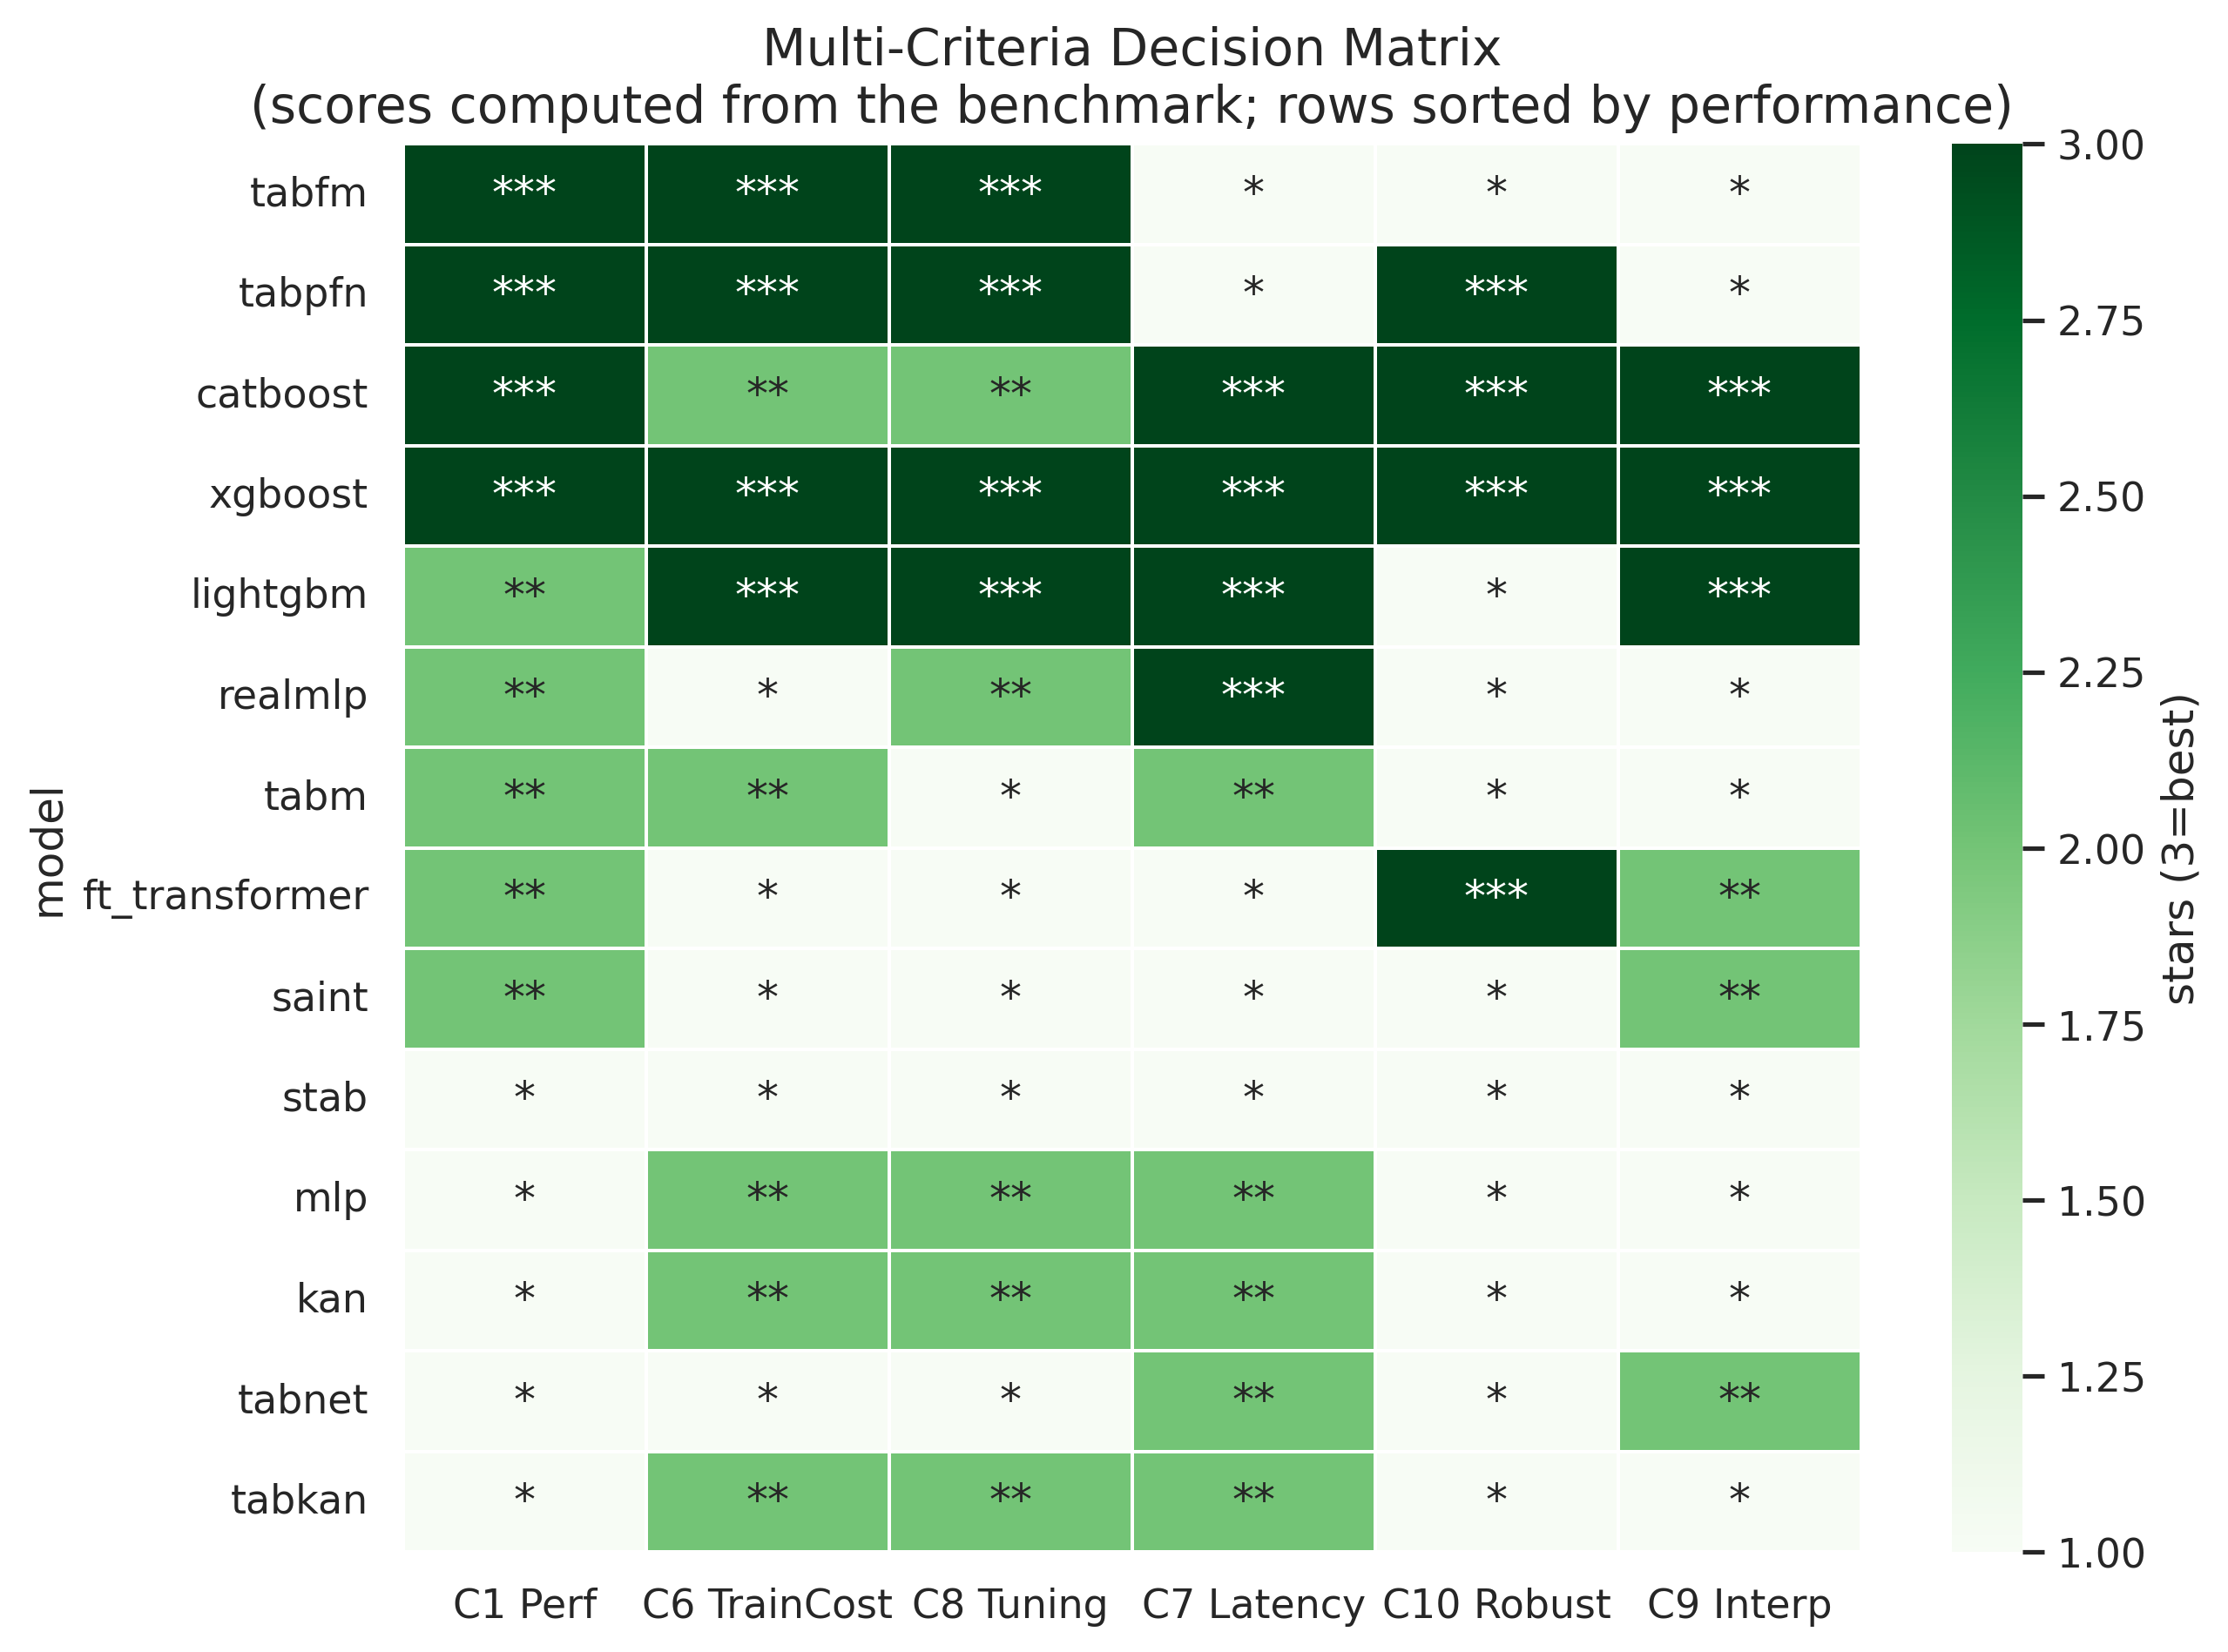
\includegraphics[width=0.92\linewidth]{images/decision_matrix.png}
\caption{Matriz de decisão multicritério dos 14 modelos (linhas,
ordenadas por desempenho) em seis critérios (colunas; rótulos internos da
figura em inglês). Fonte: \texttt{results/figures/decision\_matrix.png}.}
\label{fig:decision-matrix}
\end{figure}

A matriz torna visível o padrão central: as linhas do topo (foundation
models) e as do meio (GBDTs) têm perfis \emph{complementares}, não
ordenáveis --- o que é ótimo em desempenho é fraco em latência, e
vice-versa. O segundo instrumento, o fluxograma orientado a restrições
(apresentado em sua forma final na Seção~\ref{sec:arcabouco-resultante}),
codifica esse compromisso como uma sequência de perguntas verificáveis
antes de qualquer treino.

Ambos os instrumentos, porém, são descritivos: resumem o que o benchmark
mediu, mas não foram testados contra conjuntos que não participaram de
sua construção. Um arcabouço de recomendação que nunca foi exposto a
esse teste está sujeito à mesma crítica de \emph{overclaiming} que
atinge parte da literatura de recomendação de algoritmos. Este capítulo
eleva o arcabouço de descritivo a \textbf{validado} com dois resultados
complementares --- um negativo (o que o arcabouço \emph{não} deve tentar
fazer) e um positivo (a política que os dados sustentam) --- e, em
seguida, com um terceiro estudo, pré-registrado, que estende a validação
ao cenário multicritério.

\section{O resultado negativo: roteamento por meta-características não
generaliza}
\label{sec:resultado-negativo}

A literatura de meta-learning, que remonta ao problema de seleção de
algoritmos \citep{rice1976}, sugere um caminho sedutor: prever o
algoritmo vencedor a partir de meta-características do conjunto de dados ---
tamanho, dimensionalidade, desbalanceamento, fração de atributos
categóricos. Se funcionasse, o arcabouço de decisão seria um modelo
preditivo, não um fluxograma. Testamos essa promessa com o protocolo
honesto disponível para $N{=}18$ conjuntos: validação
\emph{leave-one-dataset-out} (LODO), em que uma árvore de decisão de
profundidade 2 --- o mesmo modelo ilustrativo da Figura~2.1, no
Capítulo~\ref{chap:fundamentacao} --- é treinada nos demais 17 conjuntos para
prever a família vencedora do conjunto excluído, repetindo-se o
procedimento para cada um dos 18.

O resultado contraria a expectativa criada pela literatura --- e por
isso o reportamos com o protocolo à vista. No estudo com 11 modelos
(o núcleo de 11 modelos do estudo original), a árvore atinge \textbf{taxa de acerto de 0,11 contra
0,44 do \emph{baseline} de classe majoritária}; no estudo com 14 modelos
(incluindo a geração 2026), 0,72 contra 0,78 do \emph{baseline}. Em nenhuma
das duas configurações o roteador aprendido supera a regra trivial
``preveja sempre a família que mais vence''. Investigado o porquê, a
atribuição é direta: com $N{=}18$ conjuntos, cada rodada do LODO
treina com 17 exemplos --- uma amostra em que qualquer partição por
meta-características é dominada pelo ruído das reversões individuais, e em
que o preço de errar uma folha é alto. O resumo honesto é este:
aprender o roteamento por meta-características não é viável sob LODO com essa
classe de modelo nesta escala de $N$ --- e afirmar isso sob um protocolo
explícito protege o arcabouço da crítica de \emph{overclaiming}
mencionada acima. A árvore permanece no trabalho como \emph{ilustração
descritiva da estrutura} das reversões entre famílias, jamais como
preditor.

Evidência independente e contemporânea aponta na mesma direção:
abordagens globais baseadas em meta-características não são robustas o
suficiente para explicar ou selecionar entre modelos da era dos
\emph{foundation models} tabulares \citep{herre2026}. A convergência entre
nosso protocolo LODO e um estudo externo, com metodologia distinta,
reforça que o resultado negativo não é um artefato da nossa amostra de
conjuntos.

\emph{Roteamento por meta-características não generaliza sob LODO.}
Com $N{=}18$ conjuntos, um roteador aprendido (árvore de profundidade
2) não supera o \emph{baseline} de classe majoritária em nenhuma das duas
gerações de modelos (0,11 vs.\ 0,44 com 11 modelos; 0,72 vs.\ 0,78 com
14). O arcabouço de decisão não deve conter um preditor de família
vencedora --- conclusão corroborada por evidência independente
\citep{herre2026}.

\section{O resultado positivo: a política ``FM primeiro'' e sua
evolução}
\label{sec:resultado-positivo}

Se o roteamento aprendido não funciona, a alternativa natural são
\emph{políticas fixas}: recomendar sempre a mesma família,
independentemente do conjunto. Para compará-las, usamos a métrica de
\textbf{regret normalizado} sobre a métrica primária de cada conjunto:
0 significa que a família recomendada contém o melhor modelo do
conjunto; 1, que contém apenas o pior. A
Tabela~\ref{tab:regret-lodo} resume o \emph{regret} das quatro políticas ---
a árvore sob LODO e as três políticas fixas --- nos dois estudos; as
linhas da árvore e da política sempre-FM agregam sobre os 17 conjuntos em
que a família FM participa (\texttt{helena} é excluída por limite
arquitetural de 100 classes), e as linhas sempre-GBDT e sempre-DL, sobre
todos os 18.

\begin{table}[htb]
\centering
\caption{Regret normalizado das políticas de recomendação sob LODO, nos
estudos com 11 e com 14 modelos (\textbf{negrito} = melhor política da
coluna). Fonte: \texttt{results/aggregated/lodo\_validation\{,\_14\}.csv}.}
\label{tab:regret-lodo}
\small
\begin{tabular}{lcccc}
\toprule
Política & média @11 & mediana @11 & média @14 & mediana @14 \\
\midrule
Árvore (LODO)      & 0,228 & 0,145 & 0,051 & 0,000 \\
Sempre-GBDT        & 0,249 & 0,168 & 0,305 & 0,291 \\
Sempre-DL          & 0,189 & 0,132 & 0,313 & 0,349 \\
\textbf{Sempre-FM} & \textbf{0,115} & \textbf{0,018} & \textbf{0,021} &
\textbf{0,000} \\
\bottomrule
\end{tabular}
\end{table}

Três leituras emergem da tabela. Primeiro, já no núcleo de 11 modelos do estudo original,
``usar o \emph{foundation model} por padrão'' era a melhor política fixa
(\emph{regret} médio 0,115; mediano 0,018). Segundo, com a geração 2026, o
\emph{regret} mediano da política cai a \textbf{zero}: em metade ou mais dos
conjuntos, a família FM contém o melhor modelo, ponto. A pergunta
``qual família vence?'' se dissolve --- e com ela o valor de qualquer
roteador de desempenho. Terceiro, o aparente empate entre a árvore e a
política sempre-FM na mediana @14 (ambas 0,000) merece explicação, e
ela desfaz o empate: com 14 modelos, a árvore aprende a prever a
família FM em quase todos os conjuntos, colapsando na política fixa ---
mas mantendo taxa de acerto \emph{abaixo} do \emph{baseline} de classe majoritária
(Seção~\ref{sec:resultado-negativo}). A política fixa atinge o mesmo
\emph{regret} sem esse modo de falha; o colapso da árvore é mais um sintoma de
que não há estrutura aprendível, não uma vitória do roteador.

\emph{``Foundation model primeiro'' é a política regret-ótima na
métrica primária.} Na geração 2026, a política fixa sempre-FM atinge
\emph{regret} médio 0,021 e mediano 0,000 sob LODO --- nenhuma política
aprendida ou fixa a supera. A recomendação de desempenho deixou de
depender do conjunto de dados; a ressalva é que esse resultado vale
para a métrica primária isolada, questão que a próxima seção enfrenta.

\section{Regret multicritério ponderado: quando a recomendação vira}
\label{sec:regret-ponderado}

O resultado positivo da seção anterior tem uma limitação declarada
desde o artigo AI-1: o \emph{regret} é calculado sobre a métrica primária,
não sobre combinações multicritério ponderadas por preferências do
usuário. A limitação não é cosmética. O Capítulo~\ref{chap:benchmark}
mostrou que o líder de acurácia custa 4--5 ordens de magnitude mais
para servir que um GBDT; um praticante cuja função de utilidade pondere
acurácia \emph{e} custo de inferência pode, legitimamente, chegar a
outra recomendação. Esta seção fecha essa lacuna com o experimento E2,
pré-registrado em \texttt{docs/desenho-melhorias-finais.md}
(05/10/2026, antes da execução, conforme o contrato de conduta do
programa de pesquisa): a política ``FM primeiro'' continua regret-ótima
quando a métrica de decisão pondera acurácia e custo?

\subsection{Desenho pré-registrado}
\label{sec:e2-desenho}

O desenho define um score multicritério por modelo$\times$conjunto:
\begin{equation}
S \;=\; w \cdot r_{\text{acc}} \;+\; (1-w) \cdot r_{\text{lat}},
\label{eq:score-ponderado}
\end{equation}
em que $r_{\text{acc}}$ é o rank normalizado em $[0,1]$ do modelo na
métrica primária do conjunto, $r_{\text{lat}}$ é o rank normalizado da
latência de inferência, e $w \in \{1{,}0;\, 0{,}9;\, \ldots;\, 0{,}0\}$
varre o espectro de preferências --- de ``só acurácia importa''
($w{=}1$) a ``só latência importa'' ($w{=}0$). Para cada valor de $w$,
calcula-se o \emph{regret} normalizado de cada política fixa exatamente como
no estudo original: 0 se a família recomendada contém o modelo de
melhor score $S$ no conjunto; 1 se contém apenas o pior.\footnote{As
quatro políticas do pré-registro estão no artefato
(\texttt{results/aggregated/lodo\_weighted\_regret.csv}): a árvore-LODO
é avaliada pela recomendação por conjunto armazenada no estudo original
(\texttt{lodo\_validation\_14.csv}), sem reajuste --- ela foi treinada
para prever o vencedor de \emph{acurácia} e aqui é pontuada sob o score
ponderado. O resultado antecipa a Seção~\ref{sec:resultado-negativo}:
a árvore nunca supera a melhor política fixa em nenhum $w$ e colapsa na
política sempre-FM nos pesos altos (mediana 0{,}000 apenas em
$w \geq 0{,}9$).}
Os $N$s espelham os da Tabela~\ref{tab:regret-lodo}: 18 conjuntos para
as políticas sempre-GBDT e sempre-DL, 17 para sempre-FM
(\texttt{helena} excluída por limite arquitetural). A hipótese
pré-registrada H-W1 afirma: existe $w^{*} < 1$ a partir do qual
``sempre-GBDT'' passa a ter \emph{regret} mediano menor que ``sempre-FM'' ---
o que tornaria o fluxograma (pergunta 1 = latência) a forma correta da
política, e não um refinamento cosmético.

Uma limitação do desenho foi declarada no próprio pré-registro e deve
ser repetida aqui: a latência usa como \emph{proxy} a medição
padronizada no conjunto \texttt{adult} --- a única disponível para os 14
modelos sob protocolo idêntico. A latência relativa entre modelos é
aproximadamente estável entre conjuntos para GBDTs e modelos de deep
learning; para \emph{foundation models}, porém, ela cresce com o tamanho do
contexto, de modo que o proxy é conservador a favor dos FMs em
conjuntos pequenos e contra eles em conjuntos grandes. As conclusões
desta seção devem ser lidas com essa ressalva.

\subsection{Resultados: o cruzamento}
\label{sec:e2-resultados}

A Figura~\ref{fig:lodo-weighted} mostra o que a
Tabela~\ref{tab:regret-lodo} não pode mostrar: como o \emph{regret} de cada
política evolui à medida que o peso se desloca da acurácia para a
latência --- o painel esquerdo traz a mediana e o direito, a média sobre
os conjuntos.

\begin{figure}[htb]
\centering
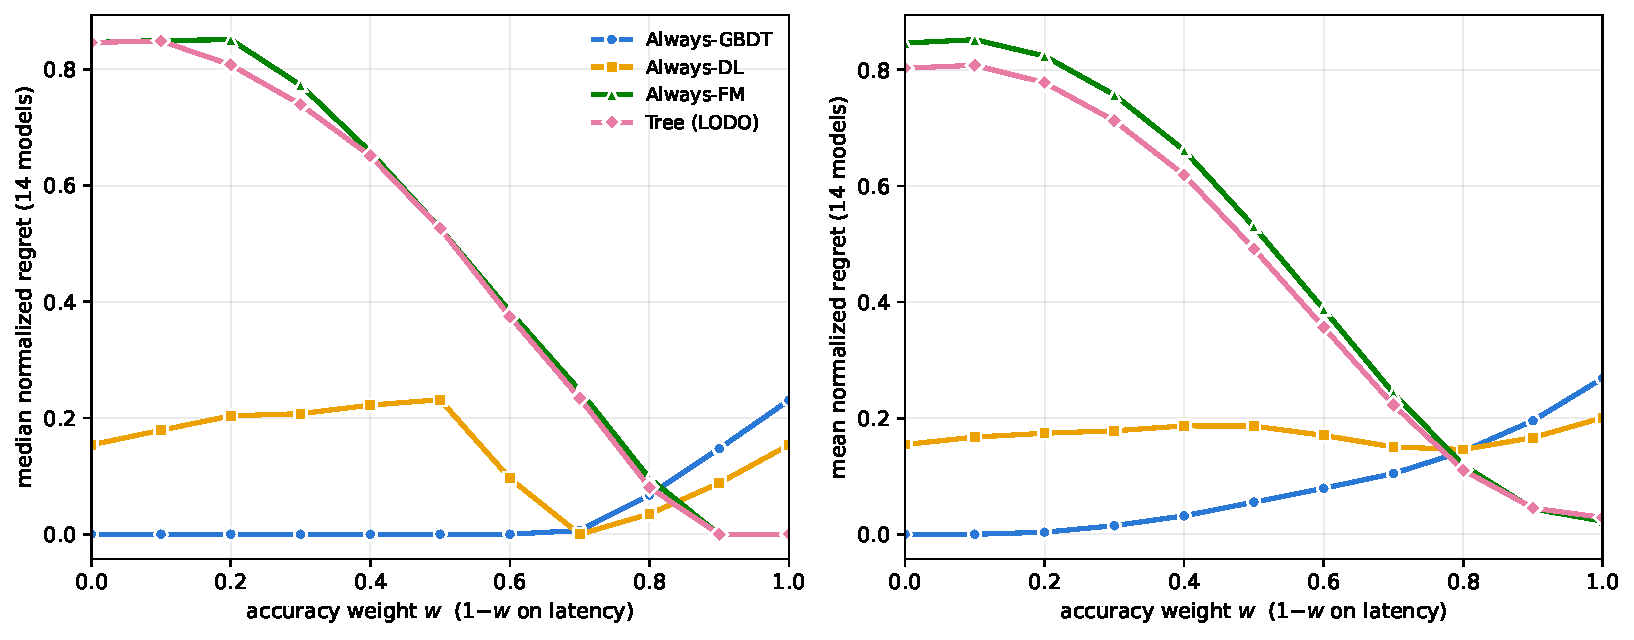
\includegraphics[width=\linewidth]{images/lodo_weighted_regret.pdf}
\caption{Regret multicritério ponderado das três políticas fixas em
função do peso da acurácia $w$ (Eq.~\ref{eq:score-ponderado}; experimento
E2, estudo com 14 modelos). Fonte:
\texttt{results/aggregated/lodo\_weighted\_regret.csv}.}
\label{fig:lodo-weighted}
\end{figure}

A Tabela~\ref{tab:weighted-regret} dá os valores exatos da mediana em
pontos selecionados da varredura, para que cada número citado a seguir
tenha origem inspecionável.

\begin{table}[htb]
\centering
\caption{Regret normalizado mediano das três políticas fixas em função do
peso da acurácia $w$ (estudo com 14 modelos; \textbf{negrito} = melhor
política da coluna). Fonte:
\texttt{results/aggregated/lodo\_weighted\_regret.csv} (medianas
recomputadas do artefato).}
\label{tab:weighted-regret}
\small
\begin{tabular}{lccccccc}
\toprule
Política & $w{=}1{,}0$ & $w{=}0{,}9$ & $w{=}0{,}8$ & $w{=}0{,}7$ &
$w{=}0{,}6$ & $w{=}0{,}5$ & $w{=}0{,}0$ \\
\midrule
Sempre-GBDT & 0,231 & 0,147 & 0,067 & 0,007 & \textbf{0,000} &
\textbf{0,000} & \textbf{0,000} \\
Sempre-DL   & 0,154 & 0,088 & \textbf{0,035} & \textbf{0,000} & 0,096 &
0,232 & 0,154 \\
Sempre-FM   & \textbf{0,000} & \textbf{0,000} & 0,096 & 0,248 & 0,383 &
0,526 & 0,846 \\
\bottomrule
\end{tabular}
\end{table}

A leitura conjunta da figura e da tabela estabelece três fatos.
Primeiro, \textbf{a hipótese H-W1 é confirmada, e o cruzamento é
precoce}: na grade de varredura, a política sempre-FM só mantém \emph{regret}
mediano zero em $w \in \{0{,}9;\, 1{,}0\}$. Já em $w^{*}{=}0{,}8$ ---
apenas 20\% do peso na latência --- tanto sempre-GBDT (0,067) quanto
sempre-DL (0,035) têm \emph{regret} mediano menor que sempre-FM (0,096); o
cruzamento, portanto, ocorre entre $w{=}0{,}9$ e $w{=}0{,}8$. Pela
média (painel direito da Figura~\ref{fig:lodo-weighted}), o quadro é
ligeiramente mais favorável aos FMs: sempre-FM ainda é a melhor
política em $w{=}0{,}8$ (0,119 contra 0,143 do GBDT e 0,146 do DL) e
só perde em $w{=}0{,}7$ (0,243 contra 0,105 do GBDT). Segundo, a partir
de $w \leq 0{,}6$, ``sempre-GBDT'' tem \emph{regret} mediano exatamente zero ---
assim que a latência domina a função de utilidade, a família GBDT
contém o melhor modelo em metade ou mais dos conjuntos, espelhando no
extremo oposto o que a família FM faz em $w{=}1$. Terceiro, no extremo
$w{=}0$ (só latência), o \emph{regret} mediano de sempre-FM atinge 0,846: a
família que contém o melhor modelo em acurácia contém quase o pior em
custo de inferência, o retrato numérico do compromisso que a
Figura~\ref{fig:decision-matrix} mostrava em estrelas.\footnote{Em
$w{=}1{,}0$, o score da Eq.~\ref{eq:score-ponderado} reduz-se ao rank
da métrica primária; os valores diferem marginalmente dos da
Tabela~\ref{tab:regret-lodo} (\emph{regret} médio de sempre-FM 0,023 aqui
contra 0,021 lá) porque o \emph{regret} do estudo original é normalizado na
escala da métrica primária, e o de E2, na escala de ranks. As medianas
coincidem em 0,000.}

A interpretação pré-fixada no registro do experimento aplica-se
diretamente: qualquer que fosse $w^{*}$, o resultado enriqueceria o
arcabouço ao quantificar o \emph{trade-off} que ele já codificava
qualitativamente. O valor encontrado --- cruzamento entre $w{=}0{,}9$ e
$w{=}0{,}8$ pela mediana --- faz mais que enriquecer: ele explica
\emph{por que a primeira pergunta do fluxograma é a latência}. Se a
recomendação só se sustentasse com 99\% do peso em acurácia, a pergunta
de latência seria um detalhe de borda; como ela vira com 10--20\% de
peso na latência, a pergunta é o eixo da decisão. O fluxograma da
próxima seção não é uma heurística decorativa em torno de uma política
única --- é a codificação da fronteira que a
Figura~\ref{fig:lodo-weighted} mede. Dito de outro modo: antes de E2,
sabíamos que a latência \emph{importava} (a matriz da
Figura~\ref{fig:decision-matrix} já o mostrava em estrelas); depois de
E2, sabemos \emph{quanto} ela precisa importar para mudar a resposta ---
e a resposta é: pouco.

\emph{A recomendação ``FM primeiro'' inverte-se com 10--20\% de
peso na latência.} Sob o score ponderado
$S = w \cdot r_{\text{acc}} + (1-w) \cdot r_{\text{lat}}$, a política
sempre-FM só é regret-ótima na mediana para $w \geq 0{,}9$; em
$w{=}0{,}8$ já é superada por sempre-GBDT e sempre-DL, e para
$w \leq 0{,}6$ ``sempre-GBDT'' tem \emph{regret} mediano zero. A ressalva
acompanha o achado: a latência usa o proxy padronizado do
\texttt{adult}, conservador a favor dos FMs em conjuntos pequenos e
contra eles em grandes.

\section{O arcabouço resultante: decisão por restrições}
\label{sec:arcabouco-resultante}

Os três estudos convergem para uma mesma conclusão: o que resta de
informativo na decisão --- e o que o fluxograma sempre codificou --- são
\textbf{restrições verificáveis \emph{a priori}}, não predições de
desempenho. A Figura~\ref{fig:flowchart-14} apresenta o fluxograma
validado na sua forma final, com os 14 modelos do estudo completo.

\begin{figure}[htb]
\centering
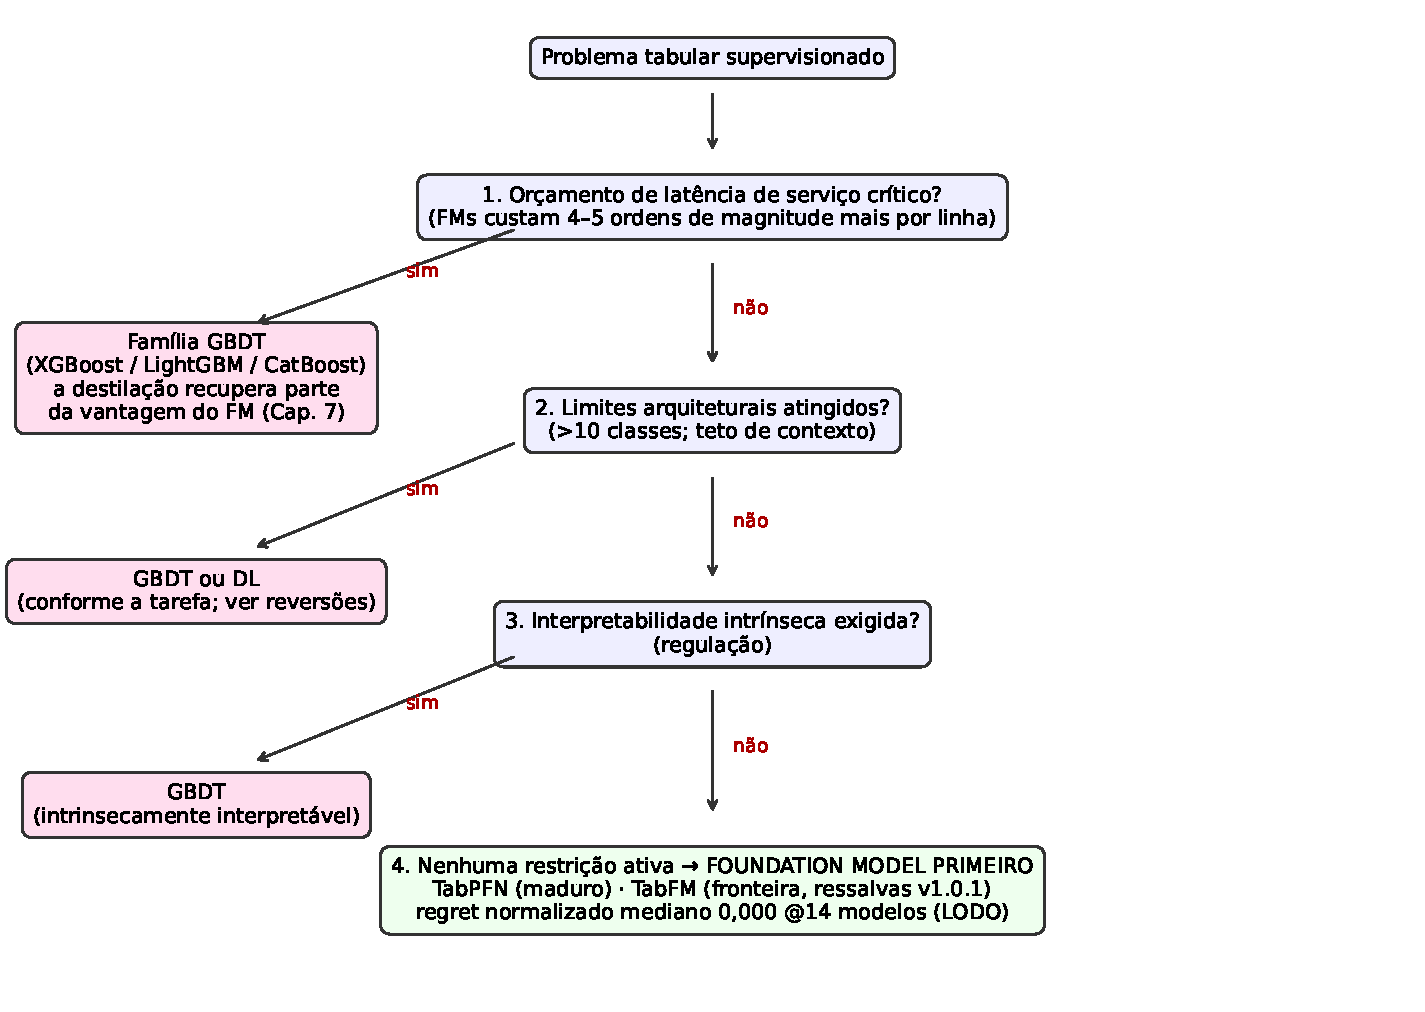
\includegraphics[width=0.88\linewidth]{images/decision_flowchart_14_pt.pdf}
\caption{Fluxograma de decisão validado, estudo com 14 modelos: cada
losango é uma restrição verificável \emph{a priori}. Gerado por
\texttt{scripts/figures\_ai1\_display.py}.}
\label{fig:flowchart-14}
\end{figure}

As quatro restrições, na ordem em que o fluxograma as verifica:

\begin{enumerate}
  \item \textbf{Latência e custo de inferência.} O líder de acurácia
    custa 4--5 ordens de magnitude mais para servir
    (Capítulo~\ref{chap:benchmark}); se o orçamento de latência é de
    microssegundos, a família FM está excluída na forma nativa. O
    experimento E2 quantifica por que esta é a primeira pergunta: a
    recomendação inverte com apenas 10--20\% do peso na latência
    (Seção~\ref{sec:regret-ponderado}). Recuperar a família FM dentro
    desse orçamento é precisamente o objeto do
    Capítulo~\ref{chap:destilacao}.
  \item \textbf{Limites arquiteturais.} Mais de 10 classes (limite do
    TabFM) ou estouro do limite de contexto são exclusões estruturais
    objetivas --- o caso \texttt{helena} (100 classes) no próprio
    benchmark.
  \item \textbf{Interpretabilidade intrínseca exigida.} Quando a
    regulação do domínio exige modelos intrinsecamente interpretáveis,
    a recomendação são os GBDTs --- a única família com perfil
    simultaneamente forte em latência e interpretabilidade na matriz da
    Figura~\ref{fig:decision-matrix}.
  \item \textbf{Nenhuma restrição ativa.} Aplica-se o \emph{default}
    regret-ótimo: \emph{foundation model}, com o TabPFN \citep{hollmann2025}
    como opção madura e o TabFM \citep{tabfm2026} como fronteira, com
    as ressalvas de maturidade discutidas no
    Capítulo~\ref{chap:benchmark}.
\end{enumerate}

A validação por \emph{regret} confirma que essas quatro perguntas capturam o
essencial: as restrições são o \emph{conteúdo informativo real} da
decisão, e o desempenho bruto deixou de discriminar dentro da família
líder. O arcabouço resultante é deliberadamente modesto na forma --- um
fluxograma, não um meta-modelo --- porque é essa a forma que os dados
sustentam.

\section{Limitações do arcabouço}
\label{sec:limitacoes-framework}

As limitações deste capítulo são declaradas na mesma moeda dos seus
resultados.

Quanto ao tamanho da amostra de conjuntos, $N{=}18$ impede validação
estatística fina do próprio arcabouço; o LODO é a ferramenta honesta
possível nessa escala, e é exatamente por isso que o resultado negativo
da Seção~\ref{sec:resultado-negativo} é formulado como ``não aprendível
sob LODO com esta classe de modelo'', e não como impossibilidade geral.

Quanto à métrica, o estudo original calcula o \emph{regret} sobre a
métrica primária. A extensão multicritério da
Seção~\ref{sec:regret-ponderado} fecha parte dessa lacuna, mas herda
duas simplificações próprias: o score pondera apenas dois critérios
(acurácia e latência) de uma função de utilidade que, na prática, pode
incluir custo de treino, robustez e interpretabilidade; e a latência
entra pelo proxy padronizado do \texttt{adult}, medido em uma única
máquina declarada --- a direção do viés desse proxy é conhecida e foi
declarada no pré-registro, mas sua magnitude por conjunto não foi
medida.

Por fim, a datação: a fronteira de modelos muda em ciclos de meses --- a
diferença entre as colunas @11 e @14 da Tabela~\ref{tab:regret-lodo} é,
ela própria, a demonstração. O arcabouço é datado por construção e
versionado com o benchmark que o sustenta; recomendações derivadas dele
devem citar a versão do estudo (11 ou 14 modelos) a que se referem.

\section{Síntese do capítulo}

Este capítulo transformou os instrumentos descritivos do
Capítulo~\ref{chap:benchmark} em um arcabouço validado por três
estudos sob LODO: o roteamento aprendido por meta-características não
generaliza (taxa de acerto 0,11 vs.\ 0,44 com 11 modelos; 0,72 vs.\ 0,78 com
14); a política fixa ``\emph{foundation model} primeiro'' é regret-ótima na
métrica primária (\emph{regret} mediano 0,000 na geração 2026); e o \emph{regret}
multicritério ponderado, pré-registrado como experimento E2, localiza o
ponto em que essa recomendação vira --- entre $w{=}0{,}9$ e $w{=}0{,}8$
de peso na acurácia pela mediana --- e com isso justifica
quantitativamente a arquitetura do fluxograma: a latência é a primeira
pergunta porque é a que mais cedo muda a resposta. O único obstáculo que
resta entre o praticante e a política regret-ótima --- a latência de
inferência --- é o objeto do Capítulo~\ref{chap:destilacao}: destilar o
conhecimento do \emph{foundation model} em um aluno que viva no
\emph{tier} de microssegundos, preservando não só a predição pontual, mas
a distribuição preditiva completa.

\chapter{Destilação Distribucional de Foundation Models}
\label{chap:destilacao}

[Conteúdo portado de \texttt{dissertation/cap7-destilacao.md} na fase de escrita.]

\chapter{Conclusão}
\label{chap:conclusao}

[Conteúdo portado de \texttt{dissertation/cap8-conclusao.md} na fase de escrita.]


\cleardoublepage
\markboth{REFERÊNCIAS}{REFERÊNCIAS}
\bibliographystyle{abnt}
\bibliography{references}

\theappendix
\chapter{Tabelas Completas de Resultados por Dataset}
\label{app:tabelas}

[A preencher na fase de escrita.]

\chapter{Espaços de Busca de Hiperparâmetros}

[A preencher na fase de escrita.]

\chapter{Resultados Suplementares e Ablações}

[A preencher na fase de escrita.]


\end{document}
